\documentclass[12pt, a4paper, oneside]{ctexbook}
\usepackage{amsmath, amsthm, amssymb, bm, color, framed, graphicx, imakeidx, 
hyperref, mathrsfs,lipsum,fancyhdr,indentfirst,array,tabularx,float,prettyref,wallpaper}

\title{{\Huge{\textbf{工程师学院数学分析笔记\\Notes d'Analyse de l'Ecole d'Ingénieur de Chimie Pékin}}}\\
版本0.1.11(持续更新中)}
\author{Augustin}
\date{\today}
\linespread{1.5}
\makeindex
\begin{document}
\newrefformat{myref}{第\ref{#1} 节}
\maketitle

\pagenumbering{roman}
\setcounter{page}{1}

\begin{center}
    \Huge\textbf{前言}
\end{center}~\
\noindent
\textbf{特别声明:}
本讲义目前为未完成版,存在大量问题等待修正,因此请在阅读时仔细甄别.如有发现错误或任何建议,欢迎发送至zyl@buct.edu.cn\\


\indent
这本东西起源于我自己的各种杂七杂八的笔记,我想把它们整理起来,系统化并且数字化,于是在大三上学期有了一个基本的雏形。
后来我想,为什么不干脆再扩充一些,搞个讲义出来呢?这样还可以给别人看,多棒。
于是大三寒假我开始慢慢扩充这本讲义,也许会一直写下去,直到哪天我没了兴趣。

\begin{figure}[H]%插入题目的图片
  \centering
  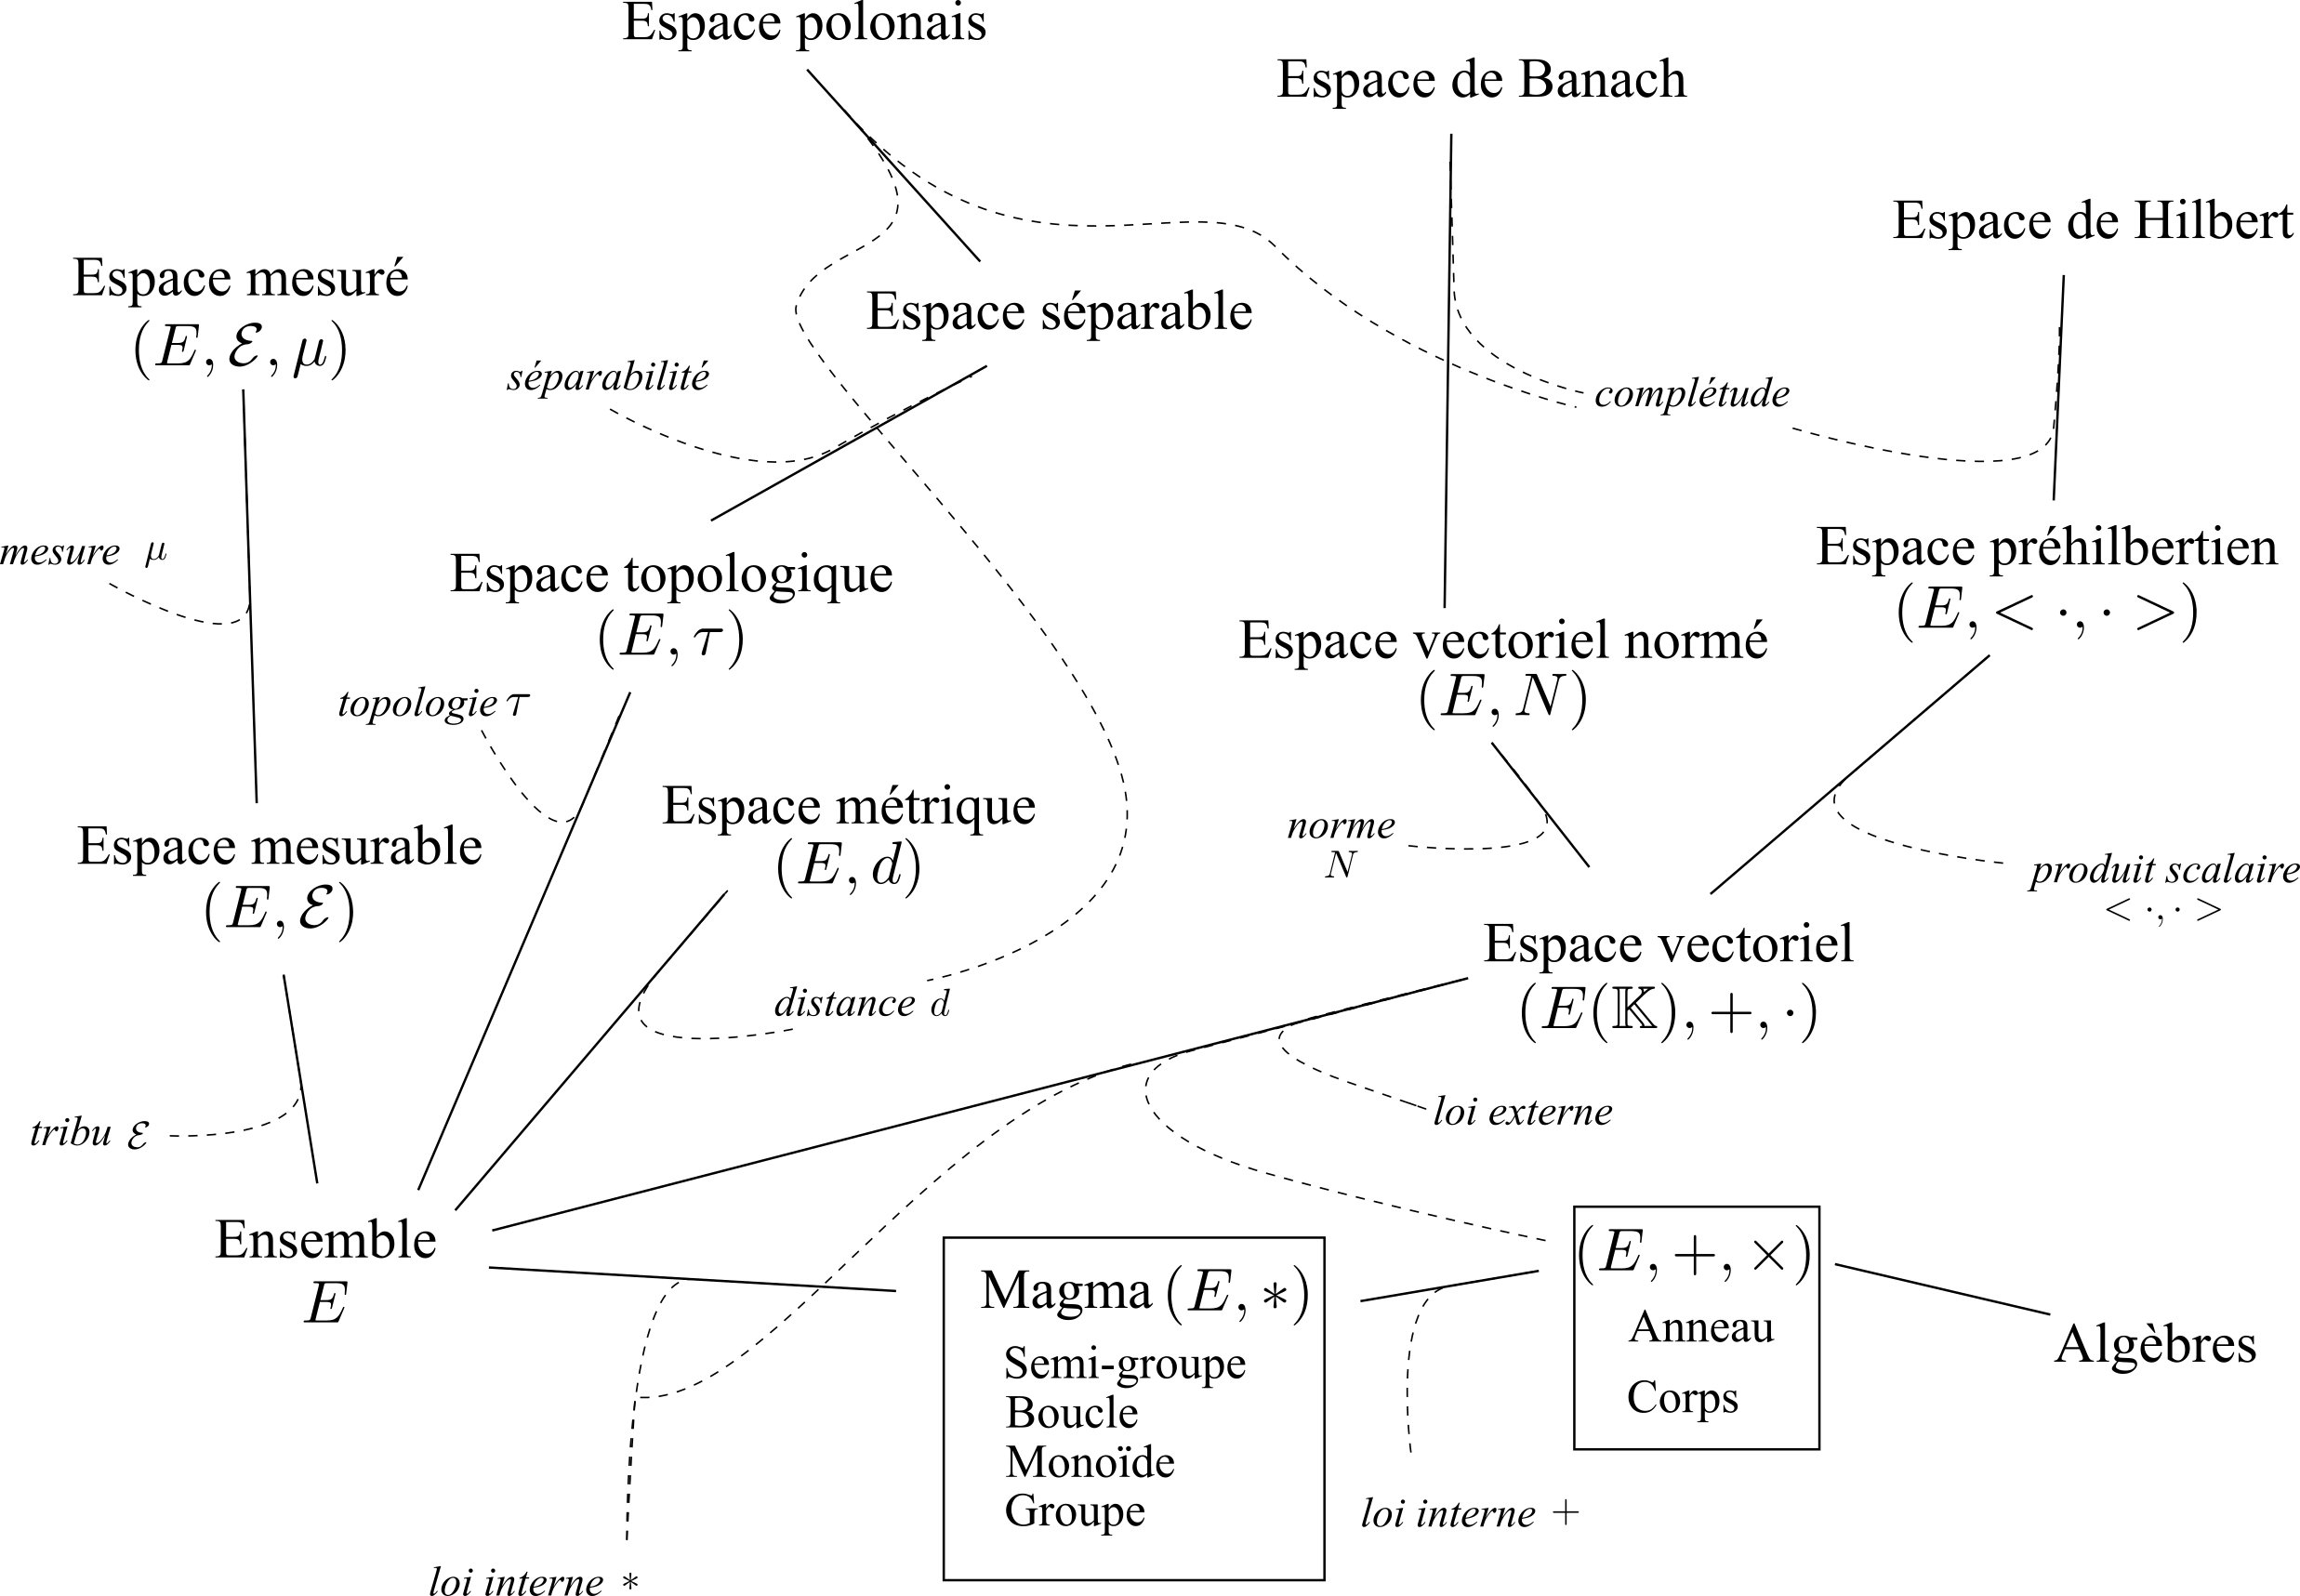
\includegraphics[scale=0.5]{abstract.png}
  \caption{数学分析部分知识关系(图源自法语wiki)}
  \label{myref:abstract}
\end{figure}

知识是网状的,而书是线性的。特别是,当你用维基百科对比一本教科书的时候,最能体现这个观点。
书的线性内容决定了作者不可能一开始就默认读者知道某个概念的所有相关概念,所以延伸性和复杂性都远远不够;而对于维基百科,就会有各种延申,每一个不知道的概念都可以点进去学习,就像是查字典。
因此任何一本书的内容都是一个线性的体系,后面的内容承接前面的内容,体现不了知识的复杂性,书的顺序也只是作者认为合理的顺序,不一定代表最适合每个读者的顺序。
所以我给出的也只是我觉得可以说得通的顺序。事实上存在大量平行的内容,相互之间怎么排列都可以。
(待更新)

讲义的定位一直在困扰我。究竟是写得简洁、方便复习的时候快速浏览知识点,还是写得详细,让没学过的人也能看懂,这是很难的取舍。
我很喜欢普林斯顿的那套数学书,各种引入、例子、详细的解释和口语化的表述读起来赏心悦目。但是我自己又写不出那种东西。
所以最后我决定开摆,写得简单并且口语化一些。本讲义大概有两种内容,即课程内容和课程的前置与延申内容。
对于课程内容,还是希望上课好好听讲,因此写的东西仅仅作为一个参考预习、复习的样例,说白了就是让你知道你学的是什么。方便读者在详细的不懂得地方可以多问老师或者自己找课程学习;
对于课外的内容,由于学院本身对于数学的要求不高,所以也只是介绍一下,并不深入。有兴趣的自己去找课程和书就行。这部分更像是一个简介,让你知道还有什么是我们没有学的,其中有哪些学一下更好。
对于讲义的参考资料,欢迎大家自己去找来看,这些东西远远比我写的精彩。我做的一点微小的工作其实就是把这些精华筛选一下,挑出我们课程用得上的东西,然后排列组合罢了。\\

\noindent
附部分讲义的参考资料与推荐阅读的资料:\\
出版物:
\begin{itemize}
  \item Proofs from THE BOOK,Martin Aigner \& Günter M. Ziegler,Springer
  \item The Princeton Companion to Applied Mathematics,Nicholas J. Higham,Princeton University Press
  \item 微积分和数学分析引论
  \item 数学分析原理,Walter Rudin,机械工业出版社
  \item 普林斯顿微积分读本,Adrian Banner,人民邮电出版社
  \item 普林斯顿线性代数读本,拉菲·格林贝格,人民邮电出版社
  \item 普林斯顿概率论读本,史蒂文·J.米勒,人民邮电出版社
  \item 代数学教程,R·戈德门特,高等教育出版社
  \item 陶哲轩实分析,陶哲轩,人民邮电出版社
  \item 数学分析中的问题和反例,汪林,高等教育出版社
  \item 拓扑空间与线性拓扑空间中的反例,汪林,高等教育出版社
  \item 实分析中的反例,汪林,高等教育出版社
  \item 泛函分析中的反例,汪林,高等教育出版社
  \item 拓扑学教程,G·肖盖,高等教育出版社
  \item 代数的历史,约翰·德比希尔,人民邮电出版社
  \item 概率论基础教程,Sheldon M. Ross,机械工业出版社
  \item 数学建模,Frank R. Giordano etc.,机械工业出版社
  \item 数学分析,B.A.卓里奇,高等教育出版社
\end{itemize}
网络资料:
\begin{itemize}
  \item \href{https://space.bilibili.com/391930545}{Maki的完美算术教室},以及\href{https://www.maki-math.com/#/}{Maki-math.com}
  \item \href{https://space.bilibili.com/1632276842}{Ayumu爱讲数学}
  \item \href{https://space.bilibili.com/29977151}{James课后习题解答}
  \item \href{https://space.bilibili.com/6073855}{Druid小德}
  \item \href{https://space.bilibili.com/3156848}{kumiko想要学分析}
  \item \href{https://space.bilibili.com/586867165}{柚柚柚子235}
  \item \href{https://space.bilibili.com/20883932}{轩兔}
  \item \href{https://space.bilibili.com/184538069}{castelu}
  \item \href{https://space.bilibili.com/88461692}{3Blue1Brown}
  \item \href{https://space.bilibili.com/415941398}{返朴科普}
  \item \href{https://zh.wikipedia.org/wiki/Wikipedia:%E9%A6%96%E9%A1%B5}{中文}、\href{https://en.wikipedia.org/wiki/Main_Page}{英语}和\href{https://fr.wikipedia.org/wiki/Wikip%C3%A9dia:Accueil_principal}{法语}的维基百科
\end{itemize}


~\\
\begin{flushright}
    \begin{tabular}{c}
        Augustin\\
        2022年12月31日
    \end{tabular}
\end{flushright}


\newpage
\begin{center}
  \Huge\textbf{版本更新说明}
\end{center}~\


\noindent
\textbf{更新内容:}\\
1.调整了章节顺序。\\
2.添加了数个章节。\\

\noindent
\textbf{计划中的更新:}\\
1.句号由"。"改为".",逗号由","改为","。\\
2.尝试加入图片。等我学会matlab再说。Manim也行。\\
3.尝试给出一些习题。\\
4.补充证明。\\
5.Bonus。\\
6.规范映射的符号$\rightarrow,\mapsto $



\newpage
\pagenumbering{Roman}
\setcounter{page}{1}
\tableofcontents
\newpage
\setcounter{page}{1}
\pagenumbering{arabic}

\part{基础知识}
\chapter{逻辑与证明\\ Logique et Démonstration}
  这一章内容是数学最基本的、最底层的概念.对于绝大多数阅读这份讲义的人而言,这些概念都是已经学习过了,或者显而易见的.
  但这并不意味着这一章的内容就很好写,或者很好讲明白.\\

  这一章(以及后面的章节里)有相当多的符号,关于这些符号的采用和相关的历史,欢迎参阅\url{https://jeff560.tripod.com/set.html}.
  \section{基本逻辑}
  首先,我假定你知道什么是“判断(Jujement)”,也就是“真(Vrai)”和“假(Faux)”的概念,否则我需要用大量笔墨来较为严谨地展现它们,并且你读起来会觉得浪费时间.
  \subsection{命题逻辑}
  命题(Proposition)是一个陈述句所表达的判断,不是真的就是假的.例如“我不懂数学”就是一个命题.当然,在本讲义中,带有Proposition节标题的内容都被认为是真的.
  \subsubsection{逻辑析取}
  定义符号$\lor $表示两个命题的逻辑析取.对于命题$p,q,\text{若}p$是真的或者$q$是真的,则$p\lor q$是真的.
  \subsubsection{逻辑合取}
  定义符号$\land  $表示两个命题的逻辑合取.对于命题$p,q,\text{若}p$和$q$都真的,则$p\land q$是真的.
  \subsubsection{逻辑否定}
  定义符号$\lnot $表示命题的逻辑否定.若命题$p$是真的,则$\lnot(p)$是假的.
  \subsubsection{逻辑蕴含}
  定义符号$\Rightarrow$表示两个命题的逻辑蕴含.对于命题$p,q$,将$p\lor(\lnot q)$记为$q\Rightarrow p$.
  表示若$q$是真的则$p$也是真的.注意,如果$p,q$都不是真的,$q\Rightarrow p$也是真的.
  \subsubsection{逻辑等价}
  定义符号$\Rightarrow$表示两个命题的逻辑等价.对于命题$p,q$,将$(p\Rightarrow q)\land (q\Rightarrow p)$记为$p\Leftrightarrow q$.
  称作p等价于q.
  \subsection{Proposition: 逻辑公理}
  公理被认为是清晰地为真的命题.以下给出逻辑的四条公理.
  \subsubsection{$AL_1$}
  $(p\lor p)\Rightarrow p$是真的.这说明,如果$(p\lor p)$为真,则$p$为真.
  \subsubsection{$AL_2$}
  $p\Rightarrow (p\lor q)$是真的.这说明,如果$p$为真,则$(p\lor q)$为真.
  \subsubsection{$AL_3$}
  $(p\lor q)\Rightarrow (q\lor p)$是真的.这说明,如果$(p\lor q)$为真,则$(q\lor p)$为真.
  \subsubsection{$AL_4$}
  $(p\Rightarrow q)\Rightarrow [(p\lor r)\Rightarrow(q\lor r)]$是真的.
  \subsection{De Morgan定律}\index{De Morgan 定律}
  数学家Augustus De Morgan发现了命题逻辑中存在着如下关系:
  \begin{itemize}
    \item $\lnot (p\wedge q)\equiv (\lnot p)\vee (\lnot q) $
    \item $\lnot (p\vee q)\equiv (\lnot p)\wedge (\lnot q) $
  \end{itemize}称为De Morgan定律,又叫对偶律.

  \section{量词 Quantificateur}
  \subsection{全称量词 Quantification Universelle}
  全称量词$\forall$表示“对所有的(pour tout)”.由Gerhard Gentzen首先于1933年使用,将德语“一切(alle)”的首字母倒过来.

  \subsection{存在量词 Quantification Existentielle}
  存在量词$\exists$表示“存在(il existe)”.由Giuseppe Peano首先于1897年使用,后被Bertrand Arthur William Russell正式用于表示“存在”.
  此外,存在量词$\exists !$表示“有且仅有唯一的(il existe et seul)”.


  \section{证明 Démonstration}
  给定命题$p$,现在并不清楚命题是真是假.如果我们想要命题为真,就需要从逻辑上证明.同理,如果想要为假,也要从逻辑上证伪.这些都属于证明.
  \subsection{逻辑变换}
  蕴含命题$p\Rightarrow q$,全称命题$\forall x,p(x)$和存在命题$\exists x,q(x)$有如下的逻辑变换:
  \subsubsection{逆命题 Implication Réciproque}
  蕴含命题$p\Rightarrow q$的逆命题为$q\Rightarrow p$,逆命题不受量词影响,即$\forall x,p(x)\Rightarrow q(x)$的逆命题为$\forall x,q(x)\Rightarrow p(x)$.
  \subsubsection{否命题 }
  蕴含命题$p\Rightarrow q$的否命题为$\lnot p\Rightarrow \lnot q$.
  全称命题$\forall x,p(x)$的否命题为$\exists x,\lnot p(x)$,
  存在命题$\exists x,q(x)$的否命题为$\forall x,\lnot q(x)$.
  \subsubsection{逆否命题 Proposition Contraposée}
  蕴含命题$p\Rightarrow q$的逆否命题为$\lnot q\Rightarrow \lnot p$.逆否命题与原命题等价.
  

  \subsection{三段论 Syllogisme}
  三段论是涉及三个命题的论证,形式如$[(A\Rightarrow B)\land (B\Rightarrow C)]\Rightarrow (A\Rightarrow C)$.
  一般而言,一个三段论分为大前提(Prémisse majeure),小前提(Prémisse mineure)和结论(Conclusion)三段.
  大前提是某种普遍性质的规律,小前提是一个特殊陈述,结论就是我们要证明的内容.
  例如要证明114是偶数,我们需要:\begin{itemize}
    \item 大前提:能整除2的数是偶数.
    \item 小前提:114能整除2.
    \item 结论:114是整数.
  \end{itemize}
  三段论的每段共有四种含义,分别为:
  \begin{itemize}
    \item A:$\forall s,p(s)$.例如:所有自然数都是实数.
    \item E:$\forall s,\lnot p(s)$.例如:所有自然数都不是负数.
    \item I:$\exists s,p(s)$.例如:存在实数是自然数.
    \item O:$\exists s,\lnot p(s)$.例如:存在实数不是自然数.
  \end{itemize}
  因此一个三段论可以被简写称诸如AAA或者AEO这样的形式,共计256种!然而只有24种是有效的.在这里我就不一一列出了,有兴趣的读者自行查阅相关内容.
  下面我们直接介绍具体的证明方法.当然,如果你能将证明方法与对应的三段论结构联系起来,那是非常棒的!

  \subsection{举例证明}
  假设要证明命题“存在不可导连续函数”,我们只需要举出一个例子就行,比如绝对值函数$f(x)=|x|$.
  同理,证伪命题“所有连续函数都可导”也是这样.
  \subsection{逆否证明}
  逆否命题与原命题等价,因此只需证明或者证伪逆否命题,就能间接证明或证伪原命题.
  \subsection{反证法}
  假设我们要证明命题A为真,我们可以假设$\lnot $A为真,然后推出一个矛盾的结果$\perp $,因此$\lnot $A为假,从而证明A为真.\\
  
  
  例如,我们要证明素数有无限个.采用反证法:$\lnot(\text{素数有无限个})\Rightarrow \text{素数有有限个} $.设全体素数组成的集合$\mathbb{P}=\{p_1,p_2,\dots,p_n\}$,
  设$n=1+\prod _{i=1}^{n}p_1$,显然$n\notin \mathbb{P}$.若$n$是素数,则我们得到了一个不属于全体素数集合的素数,这显然矛盾.若$n$不是素数,对其质因数分解,选择任意一个质因子$m$.
  若$m\in \mathbb{P}$,则$m$既是$1+\prod _{i=1}^{n}p_1$的因子,又是$\prod _{i=1}^{n}p_1$的因子,因此必须是两者之差1的因子,也就是1.因此$n=m\cdot 1$,$n$显然是素数,
  所以我们又得到了矛盾的结果.所以,只能是我们的前提“素数有有限个”是错的,故素数有无限个.
  \subsection{归纳法}
  
  \subsection{分类讨论}



  
  更多关于证明的例子和技巧,可以参阅roofs from THE BOOK这本书(中文名叫《数学天书中的证明》),其涵盖了数论、几何、分析、组合数学和图论的许多精美的证明.
\chapter{集合\\ Ensembles}
  我们先从数学最基础的内容开始.前面这一部分内容在大一就已经讲过了,然而为了保持本讲义的连贯与严谨,不突兀地出现公理化集合论之类的东西,我们还是从头开始讲起.
\section{集合}
  为了便于你的理解,我们先给出集合的定义,并且顺着这些定义讨论,随后会在\prettyref{myref:gonglihua}这里把这些概念全部公理化,以求得到更深刻的理解.
  事实上,本讲义的许多内容,都是先讲个基础的概念,随后在某个内容里将这个概念公理化.
  \subsection{Définition}
  我们朴素地认为,一个集合就是将对象归类而分成为一个或数个形态各异的大小整体。
  一般来讲,集合是具有某种特性的事物的整体,或是一些确认对象的汇集.构成集合的事物或对象称为元素.集合的元素可以是任何东西.
  \subsection{集合的特性}
  集合具有以下几个特性:
  \begin{itemize}
    \item 无序性:一个集合中,每个元素的地位都是相同的,元素之间是无序的.\footnote{
      当然,如果我们在集合上定义了序,那么元素之间就可以按照序关系排序.但就集合本身的特性而言,元素之间没有必然的序.序关系将在后续阐明.
    }
    \item 互异性:一个集合中,每个元素只能出现一次,没有相同的元素出现.
    \item 确定性:给定一个集合,任给一个元素,该元素或者属于或者不属于该集合.\label{myref:quedingxing}
  \end{itemize}
  \subsection{索引族 Famille Indexée}
  若集合$I$中的每个元素,比如$i$,都对应着一个集合$A_i$,那么称$\mathscr{A}=\{A_i|i\in I\}$为集合$A$的索引族,集合$I$是其索引集.
  \subsubsection{Exemple}
  $A_n=\{1,14,n^2\}$,且有$\mathscr{A}=\{A_n|n\in [\![5,14]\!]\}$,则$\mathscr{A}$就是$A_n$的索引族,并且$\mathscr{A}=\{ \{1,14,25\}\{1,14,36\}\dots\{1,14,196\}\}$.
  \subsection{子集 Sous-ensemble}
  若集合$B$中的每个元素都属于集合$A$,则集合$B$是集合$A$的子集,则集合$A$是集合$B$的超集,记为$B\subseteq A$或者$A\supseteq B$.
  此外,若$B\subseteq A$且$A\subseteq B$,说明二者的元素相同,是同一个集合,记为$A=B$.
  \subsubsection{Proposition}
  对于任意集合$A$,有$\varnothing\subseteq A$.
  \subsection{幂集 Ensemble Puissance}
  对于任意集合$A$,其幂集为由该集合全部子集为元素构成的集合,记为$\mathcal{P},\mathcal{P}(A)=\{B| B\subseteq A\}$.
  有时也称之为ensemble des parties.

  \section{二元关系 Relation Binaire}
  \subsection{有序对 Couple}
  有序对是包含了两个元素的特殊的集合$(a,b)$.不同于一般的集合,有序对上的两个元素是有顺序的,
  分别被称为左投影和右投影,法语也叫première composante和deuxième composante.有序对的相等要求:
  $$
  (a_1,b_1)=(a_2,b_2)\Leftrightarrow (a_1=a_2)\land(b_1=b_2)
  $$有序对可以有其他有序对作为投影,所以有序对使得能够递归定义有序.
  例如,有序三元组 (a,b,c)可以定义为(a, (b,c)),一个对嵌入了另一个对.
  \subsection{Définition}
  二元关系将一个集合的元素与另一个集合的元素相关联.例如集合$X$和$Y$上的二元关系$\mathcal{R} $是一组新的有序对$(x,y)\text{组成的集合$\mathcal{G} $,其中}x\in X,y\in Y$.
  如果$(x,y)\in\mathcal{G}$,则称$x,y$有关系$\mathcal{R}$,记作$x\mathcal{R}y$或者$\mathcal{R}(x,y)$.
  \subsubsection{Exemple}
  $\mathbb{N}$上的大于关系$>$可以表示为$\{(a,b)|\exists r\in \mathbb{N},(a=b+r)\}$.记作$a>b$.
  \subsection{关系的性质}
  二元关系$R$可能拥有以下的某些性质:
  \subsubsection{自反性 Relation Réflexive}
  $\forall x\in X,(x,x)\in R$
  \subsubsection{非自反性 Relation Irréflexive}
  $\forall x\in X,(x,x)\notin R$
  \subsubsection{对称性 Relation Symétrique}
  $\forall x\in X,y\in Y,(x,y)\in R\Leftrightarrow(y,x)\in R$
  \subsubsection{反对称性 Relation Antisymétrique}
  $\forall x\in X,y\in Y,(x,y)\in R\land(y,x)\in R \Leftrightarrow x= y$
  \subsubsection{非对称性 Relation Asymétrique}
  $\forall x\in X,y\in Y,(x,y)\in R\Rightarrow (y,x)\notin R$
  \subsubsection{传递性  Relation Transitive}
  $\forall(x,y)\in R,\forall (y,z)\in R\Rightarrow(x,z)\in R$
  \subsection{等价关系 Relation d'Équivalence}
  若二元关系$\thicksim $满足自反性、传递性和对称性,则称其为等价关系,记作$a\thicksim b$.
  \subsubsection{Exemple}
  \begin{itemize}
    \item 集合的相等是等价关系.
    \item 三角形的相似关系和全等关系是等价关系.
    \item 温度相同是等价关系.
  \end{itemize}
  \subsubsection{等价类 Classe d'Équivalence}
  集合$E$上定义等价关系$\thicksim $,对$a\in E$,$a$的等价类为集合中所有与其等价的元素组成的集合$\{x|x\thicksim a\land x\in E\}$.
  
  \subsection{序关系 Relation d'Ordre}
  前文说过,集合上的元素本身是无序的,这意味着元素之间是平等的,无法比较的.
  例如给定集合$\{$2000CNY,3000USD,1919JPY,400EUR$\}$,我们并不知道四个元素分别意味着什么,也不知道他们的关系.现在给出$Champion$断言:2000CNY$\ge$3000USD.
  为什么可以这么说?显然,这说明存在某种“顺序”,这种“顺序”可以通过符号$\ge$来表示两个元素的关系.事实上,这就是一种序关系.下面我们分别介绍各种序关系.
  \subsubsection{全序关系 Relation d'Ordre Total}
  若集合$X$上的关系$\leq$满足自反性、传递性和反对称性,并且是“完全的(Totalité)”,也就是$\forall a\in X,\forall b\in X,(a\leq b)\lor(b\leq a)$.
  则称此关系为全序关系,或者非严格全序关系.\\
  
  相对应的,若集合$X$上的关系$<$定义为$a<b\Leftrightarrow \lnot(b\leq a)$,则称为严格全序关系(Ordre strict total).其满足反自反性、传递性和非对称性.
  \subsubsection{良序关系 Relation Bien Ordonné}
  若集合$X$上的全序关系$\leq$使得对任意子集$S,\exists i\in S,\forall s\in S,i\leq s$,则称此关系为良序关系.
  换句话说,任意子集有最小值的全序关系称为良序关系.

  \subsubsection{偏序关系 Relation d'Ordre Partiel}
  若集合$X$上的关系$\leq$满足自反性、传递性和反对称性,即不“完全”的全序关系被称为偏序关系.
  同理也有相对应的严格偏序关系$a<b$,使得$a<b\lor a=b\Rightarrow a\leq b$.
  \subsubsection{预序关系 Relation Préordre}
  若集合$X$上的关系$\preceq $满足自反性和传递性,则称之为一个预序关系.它既不一定是反对称的,也不一定是非对称的.
  预序关系有时也用$\lesssim $表示.将预序集的等价元素等同起来,可得到由该预序集所导出的偏序集.对称的预序就是等价关系.

\section{集合的运算}
  集合之间有以下几种常见的运算:
  \subsection{交集}
  集合$A$和$B$的交集是两者共同包含的元素组成的集合,用符号$\cap$表示,即:
  $$
  A\cap B=\{x | (x\in A)\land (x\in B)\}
  $$


  \subsection{并集}
  与交集相对应,集合$A$和$B$的并集是两者包含的所有元素组成的集合,用符号$\cup$表示,即:
  $$
  A\cup B=\{x | (x\in A)\lor (x\in B)\}
  $$

  \subsection{Remarque: 交集与并集的性质}
  \begin{itemize}
    \item 对于任意集合$A$,$A\cap A=A=A\cup A$.
    \item 交换律: $A\cap B=B\cap A,A\cup B=B\cup A$.
    \item 结合律: $(A\cap B)\cap C=A\cap (B\cap C),(A\cup B)\cup C=A\cup (B\cup C)$.
    \item $(A\cap B)\subseteq A\subseteq (A\cup B).$
    \item $A\subseteq B\Leftrightarrow A\cap B=A\Leftrightarrow A\cup B=B$.
  \end{itemize}
  \subsection{集合的分配律}
  有限个集合的交集与并集符合分配律,这是很重要的性质.对$n\in\mathbb{N}$:
  $$
  A\cup(\bigcap_{i=1}^{n}B_i)=\bigcap_{i=1}^{n}(A\cup B_i)
  $$
  $$
  A\cap(\bigcup_{i=1}^{n}B_i)=\bigcup_{i=1}^{n}(A\cap B_i)
  $$
  \subsubsection{Démonstration}
  \subsection{补集 }
  集合$A$对于集合$B$的补集是属于$B$却不属于$A$的元素组成的集合,
  记为$ \mathcal{C}_B^A$ , $A^C$或$B\backslash A$:
  $$
  B\backslash A=\{x\in B | x\notin A\}
  $$
  \subsection{差集}
  \subsubsection{对称差}

  \subsection{笛卡尔积 Produit Cartésien}
  定义两个集合的笛卡尔(Descartes)积为其元素组成的有序对的集合,即:
  $$
  X\times Y=\{(x,y)|x\in X,y\in Y\}
  $$对于同一个集合对自身做笛卡尔积,我们采用幂的符号.如$A\times A=A^2$.

  \begin{figure}[H]
    \centering
    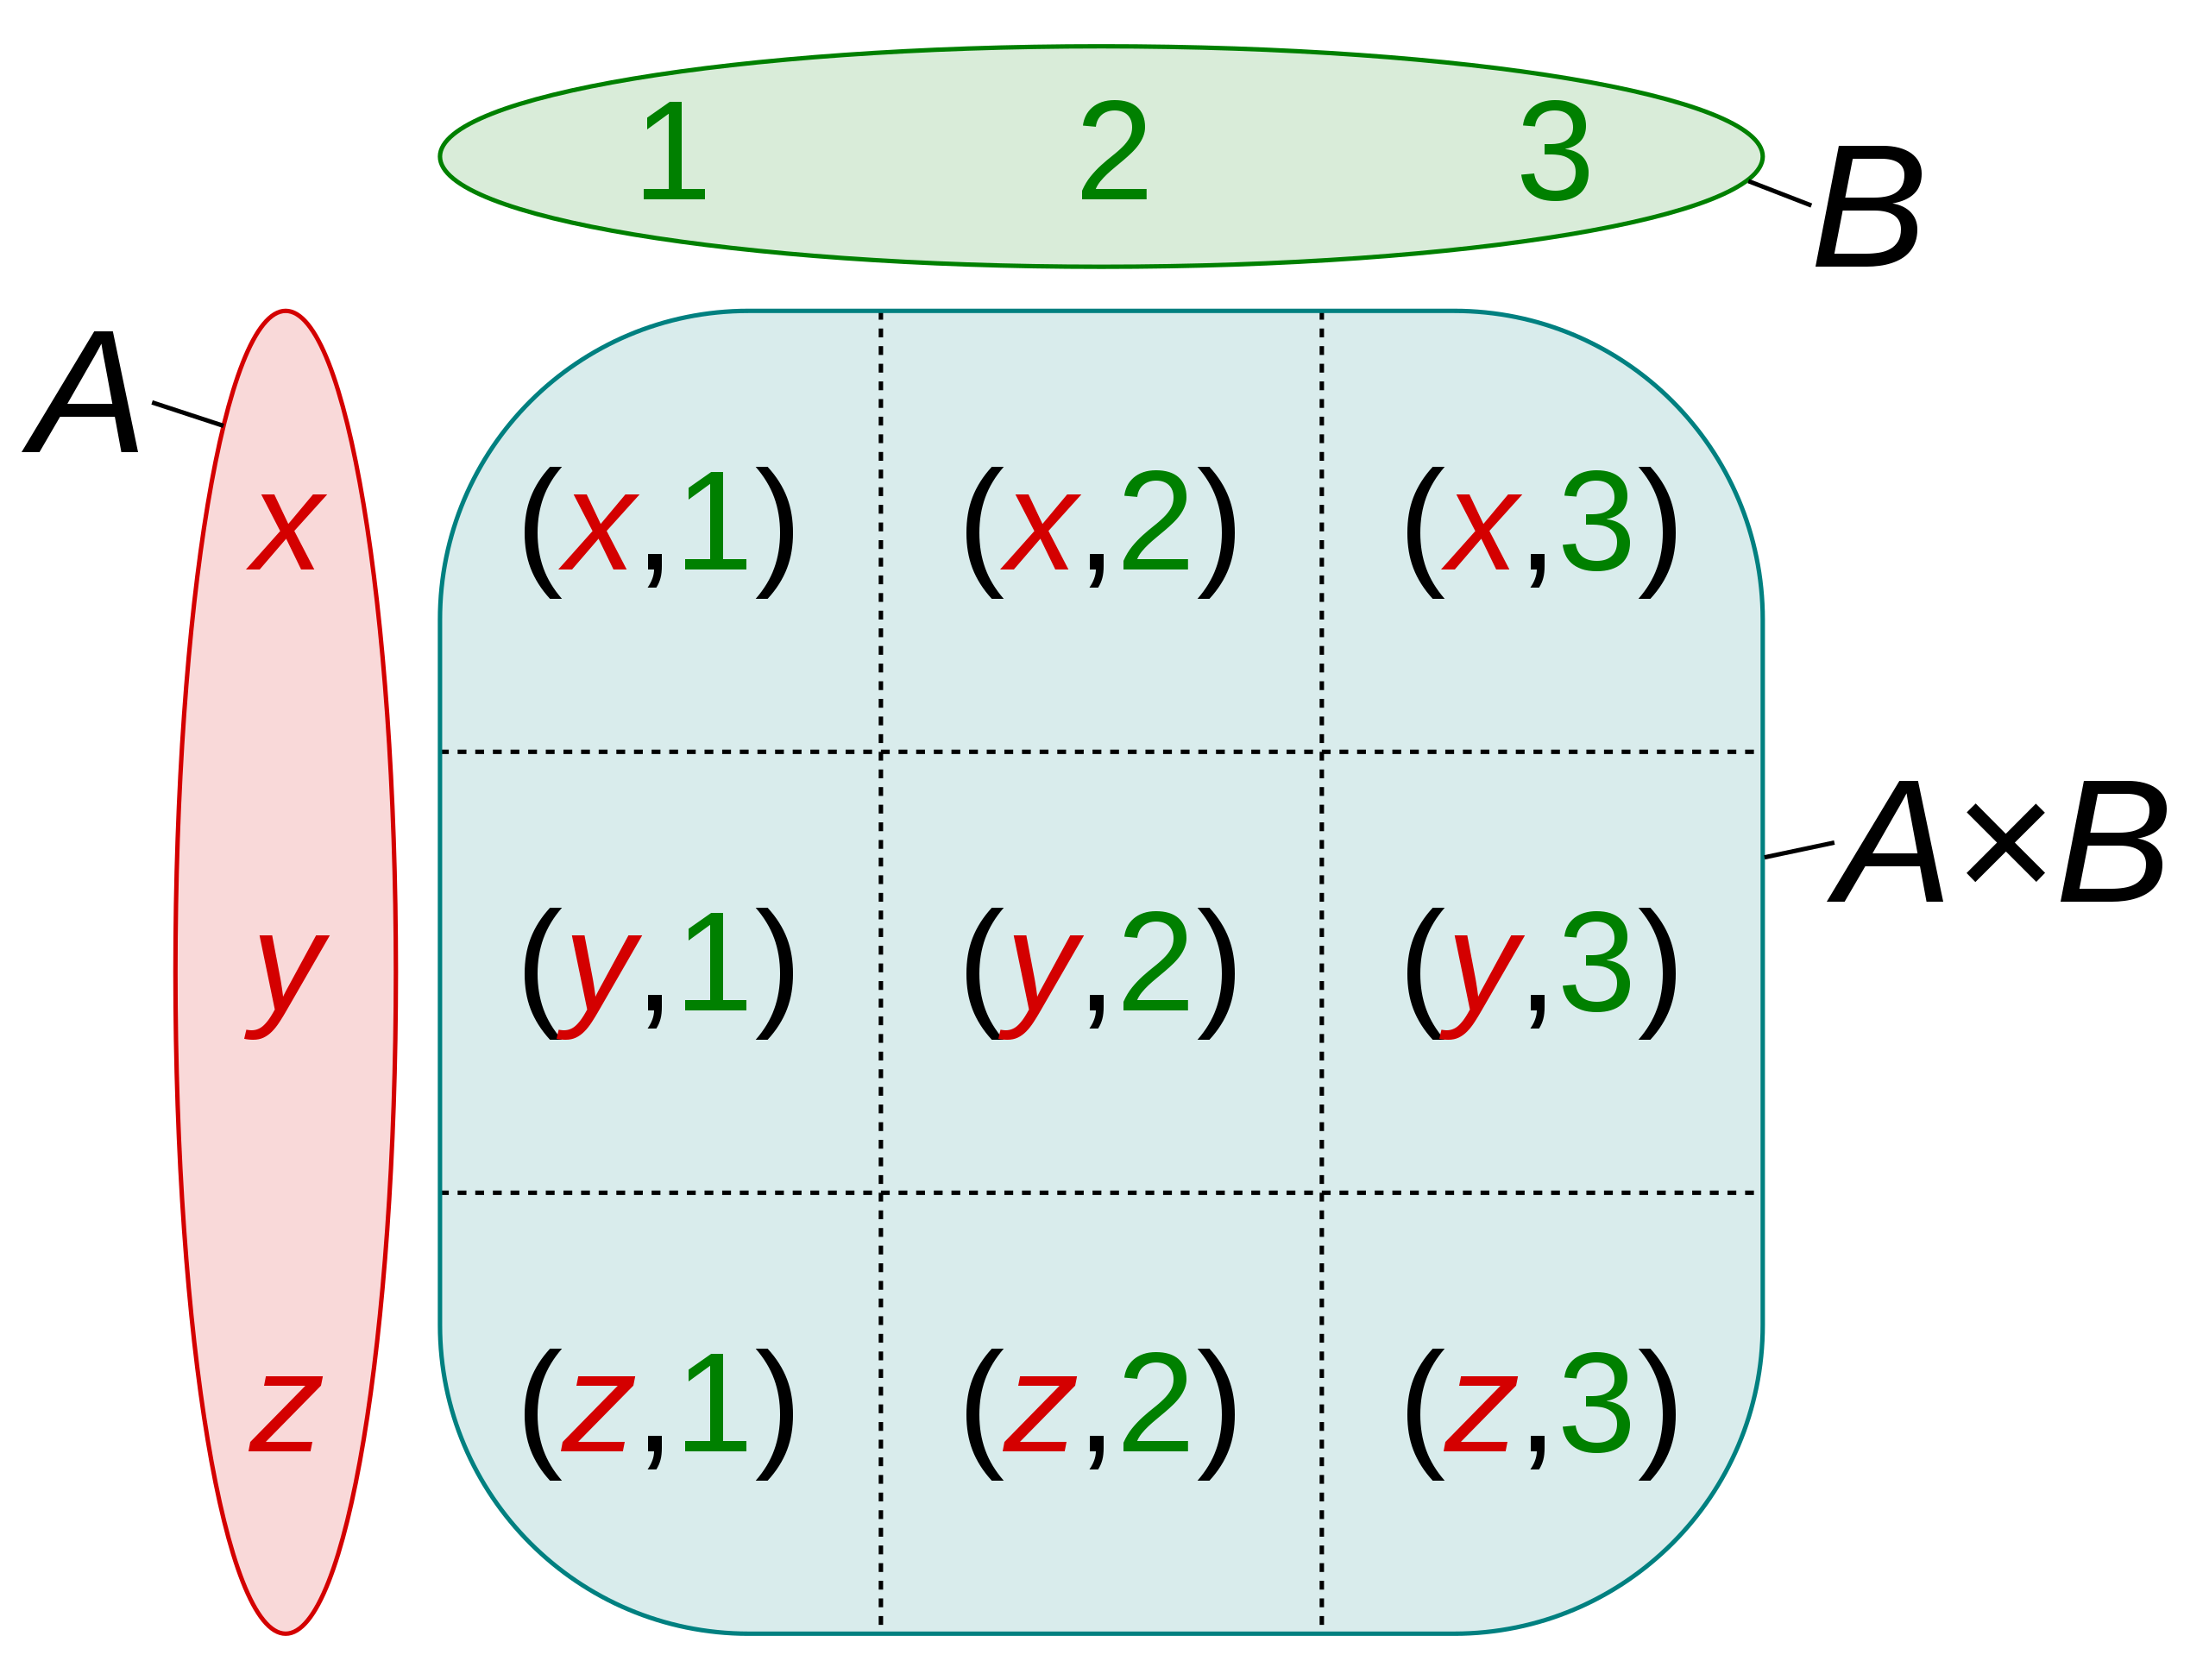
\includegraphics[scale=0.05]{Produit_Cartesien.png}
    \caption{Produit Cartésien(图源wiki)}
    \label{myref:Produit_Cartesien}
  \end{figure}
  \subsubsection{Exemple}
  我们最熟悉的平面直角坐标系就是$\mathbb{R}^2$.
  \subsection{De Morgan定律的集合形式}
  在集合论中,De Morgan定律表现为如下形式:
  \begin{itemize}
    \item $(A\cap B)^C=A^C\cup B^C $
    \item $(A\cup B)^C=A^C\cap B^C $
  \end{itemize}


  在经典命题逻辑的外延中,此二元性依然有效.即对于任意的逻辑运算符,我们都能找他它的对偶.
  这导致了基于传统逻辑的逻辑学的一个重要性质,即否定范式的存在性:如果其中否定仅出现在作用于公式中非逻辑的原子,任何公式都有它的等价公式.

  \section{公理化的集合论}\label{myref:gonglihua}
  主观意义上说,无论是ZF还是ZFC,在本讲义(或学院的课程)的“使用体验”上与原来朴素的直观的集合论没有什么区别,并且,有很多概念我们没有清晰.
  因此其实不必看懂这一章讲了什么,它不会影响你对后续章节内容的理解.
  \subsection{Russell悖论}
  现在,回头看看\prettyref{myref:quedingxing},尝试回答以下问题:\\
  设集合$A$是所有不属于自身的集合的集合,即$A=\{x | x\notin x\}$.那么请问$A$是否属于它自己?
  \begin{itemize}
    \item $A\in A$,说明$A$满足不满足其定义的不属于自身的性质,则$A\notin A$.
    \item $A\notin A$,说明$A$满足不属于自身的性质,则$A\in A$.
  \end{itemize}


  该悖论由数学家Bertrand Arthur William Russell提出,故称为Russell悖论.从经典逻辑的爆炸原理来看,任何命题都可以从矛盾中得到证明.
  因此,存在像Russell悖论这样的矛盾是灾难性的,因为如果任何公式可以被证明为真,它就破坏了真和假的含义.
  此外,由于集合论被视为所有其他数学分支公理化发展的基础,Russell悖论威胁到了整个数学的基础
  \footnote{
    其实除了Russell悖论,还有Burali-Forti悖论和Cantor悖论,但是相关的前置内容没有涉及,所以不放在这里讨论.
  },这激发了发展无矛盾的集合论的大量研究.
  \subsection{Zermelo-Fraenkel集合论:ZF公理体系}
  Zermelo-Fraenkel公理是众多集合论公理中的一员,也是对于不需要深入学习数学(特别是集合论)的我们最常见的公理体系.这套公理体系包含以下公理:
  \begin{itemize}
    \item 外延性公理 Axiom of extensionality:\\
      如果两个集合具有相同的元素则它们相等.
      $\forall A\forall B,\forall x,(x\in A\Leftrightarrow x\in B)\Rightarrow A=B $.
    \item 正规公理 Axiom of regularity:\\
      每个非空集合$X$都包含一个元素$y$,使得$X$和$y$不相交.
      $\forall X\neq \varnothing ,\exists y\in X,y\cap X=\varnothing $.
    \item 分类公理 Axiom schema of specification:\\
      设$\mathbb{Z}$为一个集合,且$\phi$为任一个描述$\mathbb{Z}$内元素$x$的特征的性质,则存在$\mathbb{Z}$的子集$Z$包含$\mathbb{Z}$内满足这个性质的$x$.
      $\forall \{x| \phi(x) \}\subseteq \mathbb{Z},\exists Z\subseteq \mathbb{Z},Z=\{x| \phi(x)\}$.\\
      
      这样我们就可以定义空集了,例如对于集合$\mathbb{Z},\varnothing =\{x|x\in\mathbb{Z}, x\neq x\}$.
    \item 配对公理 Axiom of pairing:\\
      若$X$和$Y$是集合,则存在一个集合包含$X$和$Y$. 
      $\forall X\forall Y, \exists Z,X\in Z,y\in Z $.
    \item 并集公理 Axiom of union:\\
      对任一个集合$\mathcal{F}$,存在一个集合$A$,包含每个为$\mathcal{F}$的某个成员的成员的集合.
      $\forall \mathcal{F}\exists A,\forall F\subseteq\mathcal{F},\forall x\in F\Rightarrow x\in A $.
    \item 替换公理 Axiom schema of replacement:\\
      任何可定义函数下的集合的像也将落在集合内.
    \item 无穷公理 Axiom of infinity:\\
      存在包含无限多个元素的集合.
      设$S(X)=X\cup \{X\}.\forall X \exists \mathbb{X}, X\subseteq \mathbb{X}\Rightarrow S(X)\subseteq \mathbb{X}$.
    \item 幂集公理 Axiom of power set:\\
      对任一个集合$X$,存在一个集合$Y$为$X$的幂集的超集.
      $\forall \mathbb{X},\exists \mathbb{Y},\forall X, X\subseteq \mathbb{X}\Rightarrow X\in\mathbb{Y}$.
    \item 良序定理 Well-ordering theorem:\\
      所有集合都可以被良序排序.\footnote{若给定前八个公理,就可以找到许多个和良序定理等价的叙述,例如选择公理.}
  \end{itemize}

  Zermelo-Fraenkel集合论公理是二十世纪早期为了建构一个不会导致类似Russell悖论的矛盾的集合理论所提出的一个公理系统,简称为ZF公理.
  
  \subsection{选择公理:ZFC公理体系}
  \noindent
  选择公理 Axiom of Choice:\\
  对于所有的非空的索引族$(S_i)_{i\in I}$,存在一个索引集$(X_i)_{i\in I}$使得$\forall i\in I,X_i\in S_i $.
  它可以被理解为:给定任何非空集合的族,可以通过从每个集合中任意选择一个元素来构造一个新集合,即使其包含集合是无限的.\\

  对于Zermelo-Fraenkel集合论,若讨论的是其不包含学选择公理的形式,则称为ZF公理体系;若是其包含学选择公理的形式,则称为ZFC公理体系.
  


\chapter{映射\\ Applications}%同样这一张可以删除,或者放到前面去
内容调整中。

\chapter{可数性\\ Dénoembrabilité}
  本章将研究两种不同类型的无限集:可数集和不可数集,并阐明什么是可数,什么不可数。
\section{基数 La cardinalité}
  \subsection{Définition}
  定义关系$\sim$。基数指集合中元素的个数,又叫势
  \footnote{在某些语境下,势的概念只用于比较两个无穷集的元素多寡,而不能直接指称某集合的元素个数。在一般语境下,尤其是当一切都定义好了以后,也经常使用势作为基数的同义词}。
  对于集合A和B,若当且仅当存在双射$f:A\rightarrow B$时,称$A\sim B$,即A和B拥有相同的基数。
  \subsection{Proposition}\label{myref:youxianji}
  对有限集$A$和$B$,$\text{card}A=\text{card}B\Leftrightarrow A\sim B$。
  \subsubsection{Démonstration}
  \noindent $\Rightarrow$:\\
  设$A=\{a_1,a_2,\dots,a_n\},B=\{b_1,b_2,\dots,b_n\}$有双射$f:a_i\rightarrow b_i\Rightarrow A\sim B$\\

  \noindent $\Leftarrow$:\\
  1.$\forall x\in A, \exists y\in B,\text{使得} f(x)=y\Rightarrow\text{card}A\leq\text{card}B$\\
  2.$\forall y\in B, \exists x\in A,\text{使得} f^{-1}(y)=x\Rightarrow\text{card}B\leq\text{card}A$\\
  $\Rightarrow \text{card}A=\text{card}B$
  \subsection{Proposition}\label{myref:carddengjia}
  势是等价关系。
  \subsubsection{Démonstration}
  \noindent
  1.$A\sim A:\forall x\in A, f:x\rightarrow x$即为所求双射。\\
  2.$A\sim B\Rightarrow B\sim A: f^{-1}$即为所求双射。\\
  3,$A\sim B,B\sim C\Rightarrow A\sim C:f:x\rightarrow y,g:y\rightarrow z,f\circ g $即为所求双射。\\
  
\section{可数性}
  可数性的定义非常贴近生活。想一想,平时你怎么计数?比如数一数本讲义共有几章呢?1,2,3,4,...
  计数的记号显然属于自然数集合$\mathbb{N}$。于是很自然地,我们认为一个集合如果能用自然数这样一个一个数出来,就说明它是可数的。
  \subsection{Définition}
  \noindent 
  对集合$A$,若$A\sim\mathbb{N} $称它是可数的(Dénoembrable)。\\
  若集合$A$有限或可数,称$A$是至多可数的;\\
  若集合$A$无限且不可数,称$A$是不可数的。
  \subsection{Exemple}\label{myref:Zkeshu}
  $\mathbb{Z}$是可数的。我们可以找到双射$f:\mathbb{N}\rightarrow\mathbb{Z}$:
  $$
    f(n)=\begin{cases}
    \frac{n}{2} &n=2k\\
    \frac{1-n}{2} &n=2k+1
    \end{cases}
  $$
  \subsection{Proposition}
  若$A\sim B$则$A,B$同属于"有限""无限可数""不可数"三种类型之一。
  \subsubsection{Démonstration}
  \noindent
  1.有限:见 \prettyref{myref:youxianji}\\
  2.无限可数:$A\sim \mathbb{N}$,由等价关系(\prettyref{myref:carddengjia})可知$\mathbb{N}\sim A\Rightarrow\mathbb{N}\sim B$则$B$无限可数。\\
  3.无限不可数:$\lnot(B\text{可数})\Rightarrow\mathbb{N}\sim B\Rightarrow\mathbb{N}\sim A\Rightarrow\bot$故$B$不可数。\\
  需注意:逆命题对3不成立。两个不可数集不一定能一一对应。

\section{无限集的可数性}
  \subsection{Définition}
  无限集是指至少与他的一个真子集的势相同的集合。对集合$A$,若:
  $$
    \exists B\subset A, B\sim A
  $$
  称$A$是一个无限集。
  \subsection{Exemple}
  设$S$是区间$(0,1)$上所有元素的集合,则$S$是不可数集。\\

  那么,如何证明$S$是不可数集?如果$S$是不可数集,那么当我们选取$S$的一个可数子集$E$时,$S$中应该还有一些不包含在 E 中的元素,对吧?
  也就是
  $$
    \forall E\subset S,E\sim \mathbb{N}\Rightarrow \exists x\in S,x\notin E 
  $$
  因此,如果我们可以证明$S$的每个可数子集都是一个真子集,那么$S$就是不可数集。
  这是因为如果$S$的每个可数子集都是一个真子集并且$S$是可数集,那么$S$本身就是它自己的一个真子集,这是不可能的!
  这基本上意味着无论我们如何计数$S$中的元素,总会有一些元素被漏掉。
  \subsubsection{Démonstration}
  这里我们用到了著名的Cantor对角线法。我们把每个$S$中的元素都用一个无限小数表示出来
  \footnote{我们不加证明地认为每个实数都可以写成一个无限小数},形如$0.d_1d_2d_3d_4\dots$。
  现在尝试选出可数集$E$,排列成:
  $$
  \begin{aligned}&
    e_1=0.d_{1,1}d_{1,2}d_{1,3}d_{1,4}\dots\\ &
    e_2=0.d_{2,1}d_{2,2}d_{2,3}d_{2,4}\dots\\ &
    e_3=0.d_{3,1}d_{3,2}d_{3,3}d_{3,4}\dots\\ &
    e_4=0.d_{4,1}d_{4,2}d_{4,3}d_{4,4}\dots\\ &
    e_5=0.d_{5,1}d_{5,2}d_{5,3}d_{5,4}\dots\\ &
    \vdots 
      \end{aligned}
  $$
  那么这个任意的$E$包含了$S$中的所有元素吗?错!我们可以找到这样一个数
  $$s=s_1s_2s_3s_4\dots\text{使得}s_i\neq d_{i,i}$$,
  这意味着$s$与第1个数的第1位小数不一样,与第2个数的第2位小数不一样,与第3个数的第3位小数不一样$\dots$
  也就是与$E$中每个数都不一样,显然不属于$E$。
  这里构造$s$的方法沿着上面那个有点像矩阵一样的东西的对角线一直走下去,所以叫对角线。
  该方法由集合论的创始人康托尔(Cantor)提出,故称为Cantor对角线法。
  
  \subsection{子集可数关系}
  \noindent
  设$E\subseteq A$,则有:\\
  $A\text{至多可数}\Rightarrow E\text{至多可数}$\\
  $E\text{不可数}\Rightarrow A\text{不可数}$
  \subsection{Proposition:可数集可数并可数}\label{myref:keshujikeshubingkeshu}%可数集可数并可数%
  考虑可数个集合$E_i$:
  $$
  E_i\sim\mathbb{N},S=\bigcup_{i=1}^\infty E_i\Rightarrow S\sim\mathbb{N}
  $$
  \subsubsection{Démonstration}
  有点复杂,哪天想起来再慢慢画。
  \subsubsection{Remarque}
  对于可数集的不可数并,这个结果是错误的。
  \subsubsection{Proposition}
  可数集任意可数并可数。
  \subsubsection{Proposition}
  $\mathbb{R}$不可数。
  \subsection{Proposition:可数集元组可数}\label{myref:Rnkeshu}
  设$A$是可数集,$A^n$是由$A$中元素构成的全体$n$元组的集合,那么$A^n$是可数的。
  \subsubsection{Démonstration}
  数学归纳法,先证明$A^1$可数,再假设$A^{i+1}$可数,得出$A^n$是可数集的可数并,于是$A^n$至多可数。
  详细证明留给读者。
  \subsection{Proposition:有理数集可数}
  一个简化的证明过程:我们知道任何有理数都可以写成$\frac{p}{q},(p,q)\in\mathbb{Z}^2$的形式,
  并且\prettyref{myref:Zkeshu}告诉我们$\mathbb{Z}$是可数的,\prettyref{myref:Rnkeshu}告诉我们$\mathbb{Z}^2$是可数的。
  显然$\mathbb{Z}^2$的一个子集可以与$\mathbb{Q}$构造双射,所以$\mathbb{Q}$是可数的。

  \subsection{Proposition:无理数集不可数}
  一个简单的证明过程:我们知道$\mathbb{R}=\mathbb{Q}\cup\mathbb{I}$,且$\mathbb{Q}$是可数的。
  若$\mathbb{I}$是至多可数的,则根据\prettyref{myref:keshujikeshubingkeshu}可知$\mathbb{R}$是至多可数的,这显然矛盾。
  故$\mathbb{I}$是不可数的。

  %结束了,2023新年快乐!


\chapter{运算与代数结构\\ Opérations et Structure Algébrique}
  
  \section{运算}
  在我的数学学习经历中,我最先认识了数字,也就是1、2、3、4这些,随后就开始学习了加法,然后是减法、乘法、除法之类的东西.
  这些东西都被称为运算.有些运算是一元的,例如$\cos x$和$|x|$,我们输入一个变量,得到一个返回结果;有些运算是二元(多元)的,例如$a^b$或者$A \times B$.本章里我们主要讨论二元运算.
  有些运算与数没有关系,例如逻辑运算里,$1\vee 0=1$,这里1和0只是表示逻辑上的真和假,与具体的数字无关.
  此外,还有一种题目叫做“定义新运算”,一般会给出一个自定义的算符,比如$\star $,然后解释这个算符怎么计算,比如说$a\star b=114a+\frac{514}{b}-19^{\frac{a}{b}}$,让你求解一些具体的返回值.
  这些统统都是运算.为了应付日益复杂的数学,我们需要把运算统一起来研究,以便于尝试找到普适性的规律.\label{myref:traditionalcalculate}
  \subsection{Définition}
  给定集合$X$,所有$f:X\times X\rightarrow X$的映射称为集合$X$上的运算.直观上看,运算将$X$上的有序点对映射为$X$的元素.
  我们姑且将运算符号记为$\star $.
  这样我们可以将一个运算表示为$(x,y)\in X*2,f(x,y)\rightarrow x\star y$.
  \subsubsection{Exemple}
  在$\mathbb{R}$上两个区间的并$(-114,81]\cup (-91,514)=(-114,514)$是一个运算.
  \subsection{结合律 Associative}
  设$X$上的运算$f(x,y)\rightarrow x\star y $,若:
  $$
  \forall (x,y,z)\in X^3, x\star(y\star z)=(x\star y)\star z
  $$
  称此运算满足结合律.
  \subsection{交换律 Commutative}
  设$X$上的运算$f(x,y)\rightarrow x\star y $,若:
  $$
  \forall (x,y)\in X^2, x\star y=y\star x
  $$
  称此运算满足交换律.
  \subsection{中性元/单位元 l'élément neutre/identité}
  单位元又叫中性元.设$X$上的运算$f(x,y)\rightarrow x\star y $,若:
  $$
  \forall x\in X, \exists e\in X,e\star x=x
  $$
  称$e$是左单位元,若:
  $$
  \forall x\in X, \exists e\in X,x\star e=x
  $$
  称$e$是右单位元,若$e$同时为左单位元及右单位元,则称$e$为单位元.
  \subsubsection{Exemple}
  $\mathbb{R} $上的加法单位元为0,乘法单位元为1.幂运算$a\star b=a^b$的右单位元为1,没有左单位元.
  \subsubsection{Exemple}
  集合$X$上交集运算的单位元为$X$,并集运算的单位元为$\varnothing $.
  \subsubsection{Exemple}
  设集合$A=\{e,f\}$上的运算为:
  $$
    \begin{aligned}&
    e\star e=f\star e=e\\&
    f\star f=e\star f=f
  \end{aligned}
  $$则$e,f$都是左单位元.
  \subsubsection{Proposition:单位元唯一}
  一个运算如果有单位元,则单位元是唯一的.
  \subsubsection{Démonstration}
  $\lnot (\text{单位元是唯一的})\Rightarrow \exists (e_1,e_2)\text{都是单位元}\Rightarrow e_1\star e_2=e_1,e_1\star e_2=e_2\Rightarrow e_1=e_2$
  \subsubsection{Remarque}
  一个运算有若干个左单位元是可能的.
  事实上,每一个元素都可以是左单位元.同样地,右单位元也一样.
  但若同时存在有右单位元和左单位元,则它们会相同且只存在一个单位元.
  
  \subsection{可逆元/可对称元 Symétrique}
  设$X$上的运算$f(x,y)\rightarrow x\star y $有单位元$e$,若:
  $$
  \forall x\in X, \exists x'\in X,x'\star x=e
  $$
  称$x'$是左可对称的,若:
  $$
  \forall x\in X, \exists x'\in X,x\star x'=e
  $$
  称$e$是右可对称的.所有满足$x\star x'=x'\star x=e$的$x'$称为$x$的可对称元.使用乘法符号时一般把可对称称为可逆,$x'$记作$x^{-1}$.
  
  \section{符合结合律的有单位元运算}
  符合结合律且有单位元的运算具有一些有趣的性质.本节讨论均假设$X$上满足结合律的运算$f(x,y)\rightarrow x\star y $有单位元$e$.
  \subsection{可对称元唯一性}
  当且仅当左对称元$x'$和右对称元$x''$是唯一且相同时,$x$是可对称的.
  \subsubsection{Démonstration}
  $$
    x''=e\star x''=(x'\star x)\star x''=x'\star(x\star x'')=x'\star e=x'
  $$
  \subsection{可对称的运算不变性}
  若$x$和$y$是可对称的,则$x\star y$也可对称,且$(x\star y)'=y'\star x'$.
  \subsubsection{Démonstration}
  $$
    (y'\star x')\star(x\star y)=y'\star (x'\star x)\star y=y'\star e\star y=y'\star y=e
  $$反过来同理.
  \subsection{解的唯一性}
  设$a$可对称,对于$b$,仅有唯一一个$x$使得$a\star x=b$,即$x=a'\star b$.
  \subsubsection{Démonstration}
  $$
    a\star x=b\Rightarrow a'\star b=a'\star (x\star x)=(a'\star x)\star x=e\star x=x
  $$反过来同理.
  这意味着,例如,在乘法中,形如$ax=b$的方程有且仅有唯一解$x=a^{-1}b$.

\section{代数结构 Structure Algébrique}
  在数学中,代数结构由非空集合$A$和$A$上的运算集合(通常是二元运算)和一组有限的恒等式(公理)组成,这些运算必须满足这些公理.
  研究代数结构的好处在于,当一个新问题涉及与这种代数结构相同的定律时,仅使用结构定律证明的所有结果都可以直接应用于新问题.
  \subsubsection{Exemple}
  $\mathbb{R}$上的加法$(\mathbb{R},+)$就是一个代数结构,其具有以下公理:
  \begin{itemize}
    \item 交换律:$a+b=b+a$.
    \item 结合律:$(a+b)+c=a+(b+c)$.
    \item 单位元0:  $a+0=0+a=a$.
    \item 可逆性:$a+(-a)=(-a)+a=0$.
  \end{itemize}
  \subsubsection{Exemple}
  回看前言里\prettyref{myref:abstract}所展现的分析学知识,可见大部分内容都与代数结构相关.
  \subsection{封闭性}
  当我们想使用一个代数结构,也就是对一个集合上的元素进行运算时,为了得到一些良好的性质或者进行后续的运算,
  我们通常希望运算的结果能拥有一些性质.最简单的就是这个结果可以再次被拿来运算.这意味着这个运算结果也属于代数结构的集合.
  也即$$\forall (x,y)\in A\times A, x\star y=z \Rightarrow z\in A$$这样的性质称为封闭性.


  想象一个没有封闭性的代数结构上的运算,比如$\mathbb{R}$上,某个运算结果为:$1\star 4=\text{西红柿炒鸡蛋}$.
  显然,1和4都在$\mathbb{R}$上,但是西红柿炒鸡蛋不属于$\mathbb{R}$,我们也并不清楚西红柿炒鸡蛋有什么性质,它与$\mathbb{R}$上的元素有什么关系,也不能拿来继续运算.这样的性质就很糟糕.\\
  
  现在,我希望你假装忘记掉曾经学习的这些运算,也就是\prettyref{myref:traditionalcalculate}开头我提到的那些以前的东西(特别是加法和乘法),以便我们从另一个角度重新出发学习它们.

\section{群 Groupe}
  \subsection{Définition}
  群是一种代数结构,依托于集合上的运算"$\times$",称为"乘法",记为$(G,\times)$或者$(G,\cdot)$(有时运算符号可省略).
  为了避免与笛卡尔积混淆,我们统一采用$(G,\cdot)$记号.
  其满足以下公理:
  \begin{itemize}
    \item 封闭性:$\forall(a,b)\in G^2,a\cdot b=c\in G $.
    \item 结合律:$\forall(a,b,c)\in G^3,(a\cdot b)\cdot c=a\cdot (b\cdot c) $.
    \item 单位元e: $\forall a\in G, \exists e\in G, a\cdot e=e\cdot a=a$.
    \item 可逆性:  $\forall a\in G, \exists a^{-1}\in G, a\cdot a^{-1}=a^{-1}\cdot a=e$.
    \item \textbf{Bonus:}交换律:$\forall(a,b)\in G^2,a\cdot b=b\cdot a $.
  \end{itemize}
  满足前四项公理的代数结构称为群.额外满足第五项交换律的群称为"阿贝尔群(Groupe Abélien)".
  \subsubsection{Exemple}
  \begin{itemize}
    \item 整数的通常意义加法$(\mathbb{Z},+) $构成群,但是通常意义乘法$(\mathbb{Z},\cdot) $不构成群,因为不满足有可逆元.
    \item (n阶非奇异矩阵\footnote{万一你还没学过这个定义,它意味着矩阵的行列式值不等于0.},矩阵乘法)是一个群.



  \end{itemize}
  \subsection{阶 Ordre}
  在有限群范围内,群$(G,\cdot)$的阶等于集合$G$里元素的个数,也就是$|G|=\text{card }G$.
  元素的阶等于让该元素通过幂运算得到单位元的最小幂,也就是$n_{min},a^n=e$.

  \subsection{乘法表}
  乘法表常被用来表示简单的群上的元素和运算,它列举了群内任意两个元素的乘积.下面我们通过一个简单的例子来理解乘法表.
  \subsubsection{$C_3$群}\label{myref:C_3}
  想象一个等边三角形$\Delta ABC$,我们将它绕着垂直于几何中心的州进行旋转操作:
  \begin{itemize}
    \item 操作a:顺时针旋转120°
    \item 操作b:逆时针旋转120°
    \item 操作e:不旋转
  \end{itemize}
  我们发现,经过操作a后,原来的A点变成了B点,B点变成了C点,C点变成了A点,得到了三角形$\Delta BCA$.
  而与此同时,经过两次操作b后也能让原来的A点变成了B点,B点变成了C点,C点变成了A点.也就是说,两次操作b与一次操作a等价.同理,两次操作a与一次操作b等价.
  进一步地,我们发现,三次操作a、三次操作b、操作b后操作a、操作a后操作b与操作e相互都是等价的.如果我们把操作看作一个集合,操作的复合看作运算$\cdot $,就得到了一个群.其中的运算关系如下:
    \begin{itemize}
    \item $a=b\cdot b=a\cdot e$
    \item $b=a\cdot a=b\cdot e$
    \item $e=e\cdot e=a\cdot a\cdot a=b\cdot b\cdot b=a\cdot b=b\cdot a$
    \end{itemize}
  这个群被称为$C_3$群.其阶数为3,元素a和b的阶数也是3.
  将这些运算关系组合成一个表,第一行表示在运算符号前的元素,第一列表示运算符号后的元素,就可以填入所有的运算结果.也即:
  \begin{table}[!h]
    \centering
    \begin{tabular}{r|lll}
         ($C_3,\cdot$) & \textbf{a} & \textbf{b} & \textbf{e} \\ \hline
        \textbf{a} & b & e & a \\ 
        \textbf{b} & e & a & b \\ 
        \textbf{e} & a & b & e \\ 
    \end{tabular}
    \caption{$C_3$群的乘法表}
    \label{C_3times}
  \end{table}
  \subsection{重排定理}
  考虑代数结构$(A,\star)$,对$a\in A$,定义$a\star A=\{ a\star a_\alpha|a_\alpha \in A \}$.对群$G$,有:
  $$
  \forall a\in G,a\cdot G=G\cdot a=G
  $$也即群内的每个元素和某个元素相乘得到的仍然是原来的群,这被称为群的重排定理.
  \subsubsection{Démonstration}
  由运算的封闭性知$a\cdot G\subseteq G$,
  由可逆性知$\forall (a,g)\in G\times G, \exists (a'\cdot g)\in G\text{使得}g=a\cdot (a'\cdot g)=g\Rightarrow g\in a\cdot G\Rightarrow G\subseteq a\cdot G$.
  \subsection{生成元}
  生成元是描述一个群的重要方式.下面我们由循环群开始逐渐介绍生成元和其应用方法.
  \subsubsection{循环群}
  由一个元素$R$及其幂次构成的有限群称为由$R$生成的循环群,记为$C_n$,其中$n$为循环群的阶,$R$称为循环群的生成元.
  这就是为什么\prettyref{myref:C_3}介绍的群叫$C_3$群.在$C_3$群中,a和b都是其生成元.对于$n$阶循环群, 其阶数等于其生成元的阶数.
  \subsubsection{有限群的生成元与秩}
  对任一有限群, 是否同样有生成元呢?答案是肯定的,由此还能引出有限群的秩的概念.对有限群$G$,任取一元素$R_1$,得到其幂次构成的集合$\mathbf{R_1}$.
  若$\mathbf{R_1}^C\neq \varnothing$,即无法填满整个群,则在$\mathbf{R_1}^C$内任取一元素$R_2$并得到$\mathbf{R_2}$,以此类推.
  将选取的元素组成集合$\{R_i\}$,该集合即为群$G$的生成元,且$\text{card}\{R_i\}$称为群的秩\footnote{秩这个概念经常在代数中见到,但是在分析里要等到很后面才有用.}.
  \subsubsection{Proposition}
  有限群的生成元的选择不唯一,但秩不变.

  \section{弱化:从原群到群}
  一个代数结构想成为群需要符合四个条件,那不能全部符合四个条件的代数结构又是什么呢?
  \subsection{原群 Magma}
  对代数结构$(E,\star)$,若其运算满足封闭性,则该代数结构为一个原群.

  \subsection{半群 Demi-groupe}
  对原群$(E,\star)$,若其运算满足结合律,则该原群为一个半群.

  \subsection{幺半群 Monoïde}
  对半群$(E,\star)$,若其含有中性元,则该半群为一个幺半群.

  \subsection{拟群 Quasigroupe}
  对原群$(E,\star)$,若有:
  $$
  \forall (a,b)\in E\times E, \exists (x,y)\in E\times E\text{使得}a\star x=y\star a=b
  $$则该原群为一个拟群.


  \begin{figure}[H]
    \centering
    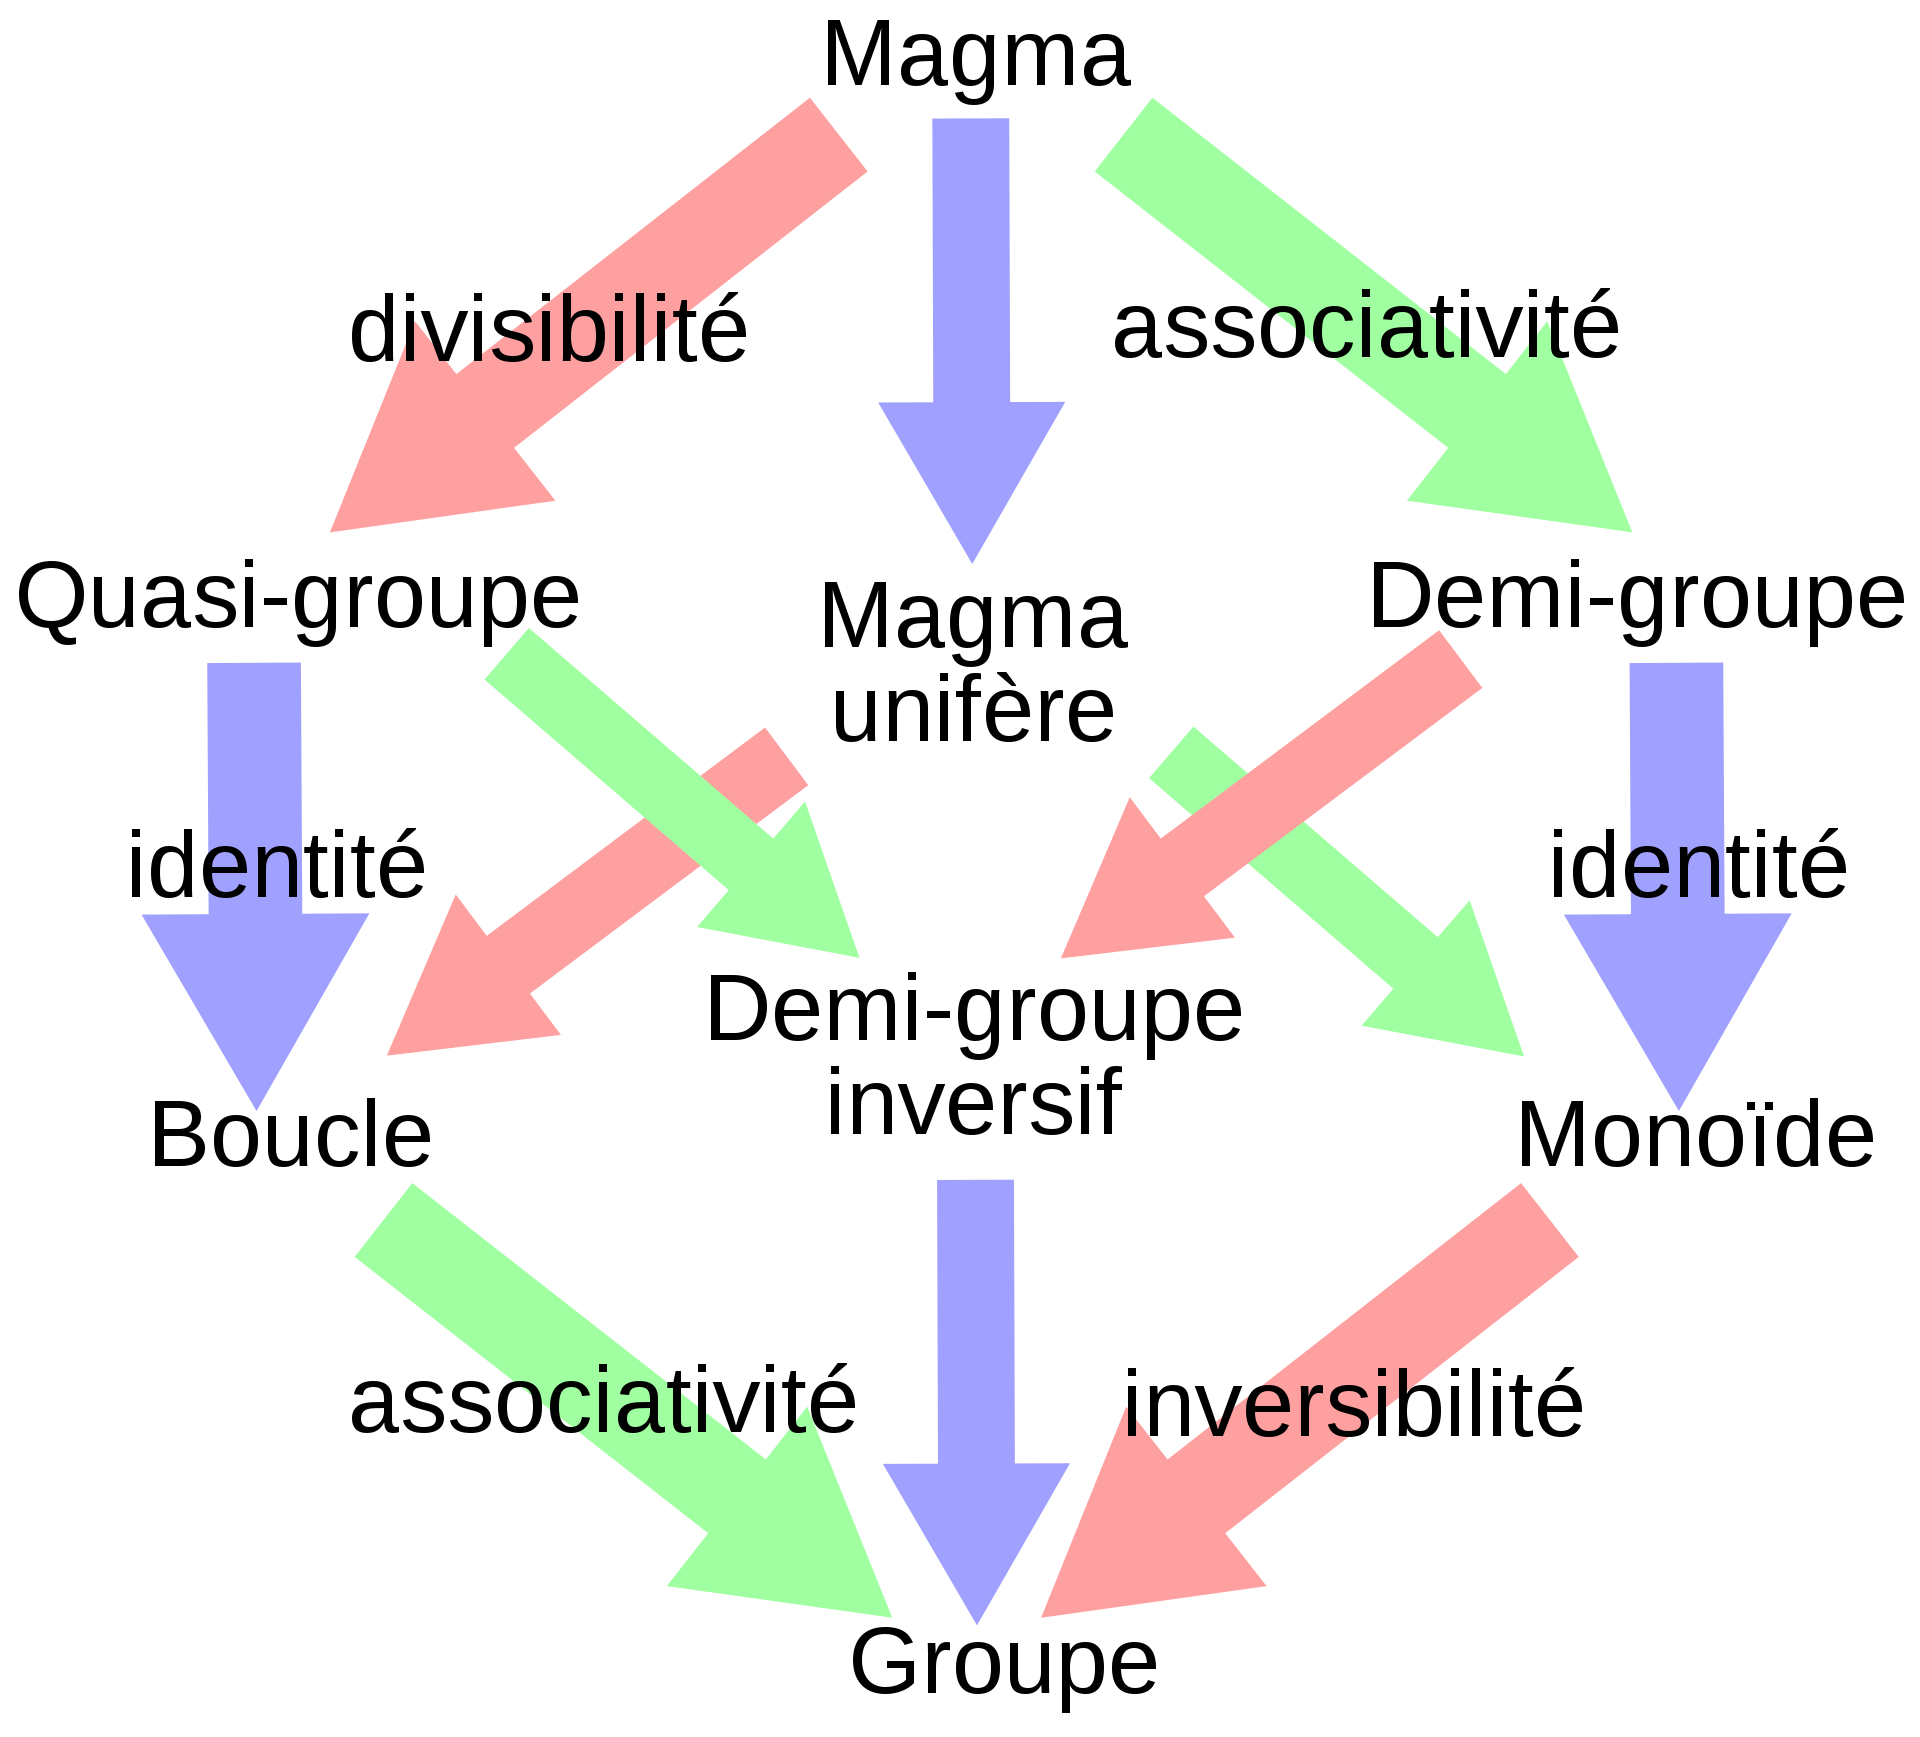
\includegraphics[scale=0.13]{magma_groupe.png}
    \caption{从原群到群(图源wiki)}
    \label{myref:groupe_magma}
  \end{figure}

  \section{群论基础 La Théorie Rudimentaire des Groupes}
  在数学中,特别是在一般代数中,群论是研究群的代数结构的学科。群论的发展起源于数论、代数方程理论和几何学,在理论物理、化学、材料科学和非对称密码学中有多种应用.
  本章只对群论内容做一个基础的、入门的介绍.事实上,关于群、环和域相关的知识在本讲义中并不怎么重要,很多结论也不会有后续应用(所以有相当多平凡的推论我没有写出证明,摸了).但是有些概念和定义还是会用上的,因此我还是简单地列出来.

  \subsection{共轭关系 Conjugaison}\label{myref:conjugaison}
  定义二元关系~为:对$(a,b)\in G\times G, \exists g\in G$使得$b=g^{-1}\cdot a\cdot g$.称该关系为共轭关系,a~b为a与b共轭.
  \subsubsection{Proposition}
  共轭关系是等价关系.
  \subsubsection{Démonstration}
  \begin{itemize}
    \item $a=a^{-1}\cdot a\cdot a\Rightarrow a\sim a$
    \item $a\sim b\Rightarrow b=g^{-1}\cdot a\cdot g\Rightarrow g\cdot b\cdot g^{-1}=a\Rightarrow a=(g^{-1})^{-1}\cdot b\cdot g^{-1}\Rightarrow b\sim a$
    \item $b=g^{-1}\cdot a\cdot g, c=f^{-1}\cdot a\cdot f\Rightarrow b=f\cdot c\cdot f^{-1}=g^{-1}\cdot a\cdot g\Rightarrow c=(f^{-1}\cdot g^{-1})\cdot a\cdot (g\cdot f)\Rightarrow c\sim a$
  \end{itemize}
  \subsubsection{共轭类 Action par conjugaison}
  a的共轭类是群内所有与其共轭的元素组成的集合,记为$Cl(a)$或$C_a$,即$Cl(a)=\{g\cdot a\cdot g^{-1}|g\in G\}$.\\

  接下来给出一些共轭类的简单推论:
  \subsubsection{Proposition}
  $a\sim b\Leftrightarrow Cl(a)\cap Cl(b)\neq \varnothing$
  \subsubsection{Proposition}
  共轭类内元素的阶相同.
  \subsubsection{Proposition}
  单位元e只与自己共轭.
  \subsubsection{Proposition}
  Abel群里每个元素只与自己共轭.
  \subsubsection{Proposition}
  $a\sim b\Rightarrow \forall k\in \mathbb{N},a^k\sim b^k$.

  \subsection{子群 Sous-groupe}
  直观上说,子群就是群的一个同样是群的子集.
  \subsubsection{Définition}
  对群$(G,\cdot)$,若$H\subseteq G$使得$(H,\cdot)$也是一个群,则称$H$是$G$的子群.
  \subsubsection{Proposition}
  $G$和$\{e\}$显然都是子群.它们被称为平凡子群(sous-groupe trivial)或者 sous-groupe impropre.
  不是平凡子群的子群称为特征子群(sous-groupe propre).
  \subsubsection{Remarque}
  质数阶(或者1阶)循环群没有特征子群.
  \subsubsection{Proposition}
  对于$pq$阶循环群($p,q$为正整数),其只有一个$p$阶子群.该子群是由$g^q$生成的循环群.

  \subsection{陪集 Classe suivant un sous-groupe}
  法语里并没有专门的陪集的专有名词,而是直接叫classe suivant un sous-groupe,这是个很形象的说法.英语称陪集为coset,其实也和suivant有异曲同工之妙吧.
  \subsubsection{Définition}
  群$(G,\cdot)$有子群$H$.对任意$g\in G$,$H$有如下两个陪集:
  \begin{itemize}
    \item 左陪集(classe à gauche de $g$ suivant $H$): $gH=\{g\cdot h|h\in H\}$
    \item 右陪集(classe à gauche de $g$ suivant $H$): $Hg=\{h\cdot g|h\in H\}$
  \end{itemize}
  \subsubsection{陪集分解}
  群$G$可以被分解成若干个左陪集的并,或者若干个右陪集的并.对应的分解称为左/右陪集分解.即:
  $$
  G=\bigcup_{\alpha\in G}\alpha H= \bigcup_{\alpha\in G}H\alpha
  $$
  \subsubsection{Proposition}
  $f\in gH\Leftrightarrow fH=gH,f\in Hg\Leftrightarrow Hf=Hg$.
  \subsubsection{Proposition}
  $gH=H\Leftrightarrow g\in H\Leftrightarrow Hg=H$.
  \subsubsection{Proposition}
  $|gH|=|H|$
  \subsubsection{Proposition}
  “属于同一左陪集”是一个等价关系.
  \subsubsection{Proposition}
  任意两个左陪集要么不相交要么相等.

  \subsection{群论的Lagrange定理}
  Lagrange定理的直接叙述为:子群的阶整除群的阶,即:若群$(G,\cdot)$有子群$H$,则$|G|=k|H|,k\in\mathbb{N}$.
  将其倍数$k$记为$[G:H]$,表示$H$在$G$中左陪集的个数.
  \subsubsection{Démonstration}
  考虑子群$H$关于$G$内所有元素的左陪集组成的集族$\mathbb{H}=\{g_iH|g_i\in G\},\text{每个左陪集的阶都相同,}|g_jH|=|g_kH|$并且$\sum_{i}^{\text{card }\mathbb{H}}|g_iH|=|G|$
  此时$\text{card }\mathbb{H} $就是$[G:H]$.
  \subsubsection{Proposition}
  素数阶的群只有平凡子群,没有特征子群.
  \subsubsection{Proposition}
  元素的阶整除群的阶.(元素的阶可以组成子群)
  \subsubsection{Proposition: Fermat小定理}
  对整数$a$和素数$p$,若$a$不是$p$的倍数,则$a^p-1$是$p$的倍数,即:
  $$
    a^{p-1}\equiv 1(\mod p)
  $$
  \subsubsection{Démonstration}
  为了证明这个推论,我们考虑$G=\{1,2,\dots , p-1\}$和模运算组成的群.假设$a\equiv b(\mod p),\text{显然}b\in G$.
  设$b$的阶数为$k$,即$b^k\equiv 1(\mod p)$,则可得到子群$H=\{a,b,\dots ,b^{k-1}\}$则$k$可以整除$G$的阶数,也就是$p-1$.
  此时再设$p-1=km$,此时有:
  $$
    a^{p-1}\equiv b^{km}\equiv (b^k)^m\equiv 1^m\equiv 1(\mod p)
  $$得证.
  \subsection{正规子群 Sous-groupe normal}
  正规子(Sous-groupe normal) 又叫不变子群(Sous-groupe invariant),法语里还有称Sous-groupe distingué.其代表共轭变换下不变的子群.
  \subsubsection{Définition}
  对群$(G,\cdot)$,若子群$N$满足:
  $$
  \forall n\in N,\forall g\in G,g\cdot n\cdot g^{-1}\in N
  $$则称$N$是$G$的正规子群,记作$N\lhd G$或者$N\unlhd G$.
  \subsubsection{等价条件}
  下列条件等价于子群N在G中是正规子群:
  \begin{itemize}
    \item $\forall g\in G,gNg^{-1}\subseteq N $
    \item $\forall g\in G,gN=Ng $
    \item $\forall (g,h)\in G\times G,gh\in N\Leftrightarrow hg\in N$
  \end{itemize}


  \subsection{商群 Groupe quotient}
  \subsubsection{子群的乘法}
  设群$(G,\cdot)\text{有子群}H\text{和}F$,定义其乘法为:
  $$
  H\cdot F=\{h\cdot f|(h,f)\in G\times F \}
  $$
  \subsubsection{Définition}
  利用正规子群的左陪集和右陪集相同的这个特点将群按照陪集的方法进行分割.
  分割后的所有陪集形成的集合能够形成一个新的群,称之为商群,记为$G/H$.也即:
  $$
  G/H=\{gH\text{ }|H\lhd G,g\in G \}
  $$
  \subsubsection{Démonstration}
  \begin{itemize}
    \item 单位元: $aH=H=Ha$
    \item 逆元: $aH\cdot a^{-1}H=aa^{-1}HH=H$
    \item 结合律: $aH\cdot bH\cdot cH=(ab)cH=a(bc)H=aH\cdot(bH\cdot cH) $
    \item 封闭性: $aH\cdot bH=(ab)H\in G/H $
  \end{itemize}
  \subsubsection{Proposition}
  $|G/H|=[G:H]$,商群的阶是群的阶除以子群的阶的商.
  \subsubsection{Proposition}
  若$(G,\cdot)$是Abel群/循环群/有限生成群,则$G/H$也是.

  \subsection{同态 Homomorphisme}    \label{myref:Homomorphisme}
  \subsubsection{Définition}
  同态是两个群之间的一种特殊的映射,其概念非常直观.“同”表示映射的两端有什么东西是一样的,或者不变的.“态”就是群的某种“状态”.
  群只有集合和运算两个要素,集合映射过去后不可能保持不变,那能保持的也就只有运算了.因此,同态就是两个群之间保持乘法运算的映射,即
  对于$(G,\cdot)$和$(H,\star)$上的映射$f:G\rightarrow H $,若
  $$
    \forall (x,y)\in G\times G,f(x\cdot y)=f(x)\star f(y)
  $$称$f$是$(G,\cdot)$和$(H,\star)$上的同态映射.存在同态映射的两个群是同态的.若同态是单射,则称单同态(Monomorphisme),若为满射则称满同态(Épimorphisme).
  \subsubsection{Exemple}
  正实数上通常加法群到通常乘法群上的映射$f(x)=e^x$就是一个同态.$e^{a+b}=e^a\cdot e^b$.
  \subsubsection{Proposition}
  同态的一个重要性质是保证了单位元映射到单位元,$f(e_G)=e_H$.
  \subsubsection{自同态 Endomorphisme}
  群$(G,\cdot)$到自身上的同态映射称为自同态.
  \subsubsection{态射 Morphisme}
  同态的推广被称为态射.在讨论群的内容时,法语有时直接用态射指代同态,记住两者在此时是同一概念.
  \subsection{同构 Isomorphisme}    \label{myref:Isomorphisme}
  若同态映射$f$为双射,则称为同构映射,两个群是同构的,记作$G\cong H$.
  \subsubsection{Proposition}
  同构是等价关系.

  \subsubsection{自同构 Automorphisme}
  同理,群$(G,\cdot)$到自身上的同构映射称为自同构.
  \subsubsection{Remarque: 同构与相等}
  一般来说,如果忽略掉同构的对象的属性或操作的具体定义,单从结构上讲,同构的对象是完全等价的.
  但这并不意味着同构就是相等.例如,我们很容易知道$C_3$群可以和某个群\{西红柿炒鸡蛋,醋溜土豆丝,糖醋排骨\}同构(例如
  $f(a)=\text{西红柿炒鸡蛋},f(b)=\text{醋溜土豆丝},f(e)=\text{糖醋排骨}$),
  但这并不代表两个群,或者两个集合就是相等的.起码西红柿炒鸡蛋不在$C_3$群里面.

  \subsection{核 Noyau}
  \subsubsection{Définition}
  对于同态$f:G\rightarrow H $, $G$中映射到$H$单位元的元素称为同态的核,记作:
  $$
  \ker f=\{f(g)=e_H\text{ }|\text{ }g\in G  \}
  $$
  \subsubsection{Proposition}
  $\ker f\lhd G$,核是正规子群.
  \subsubsection{Proposition}
  $G/\ker f\cong H$,核的商群与$H$同构.\\
  
  其实到这里我想接着讲同构基本定理的,
  但是这一章内容太多了,而且毕竟不是写代数讲义,因此我们点到为止,快速过完这一章的内容.


  \section{环 Anneau}
  \subsection{Définition}
  与群类似,环也是一种代数结构,依托于集合上的运算“$+$”和“$\times$”,分别被称为“加法”和“乘法”.同样将乘法符号记为$\cdot$,
  则一个环写作$(R,+,\cdot)$.其满足以下公理:\\

  \noindent
  1.$(R,+)$是Abel群,即:
  \begin{itemize}
    \item 封闭性:$\forall(a,b)\in R^2,a+b=c\in R $.
    \item 结合律:$\forall(a,b,c)\in R^3,(a+ b)+ c=a+ (b+ c) $.
    \item 单位元0: $\forall a\in R, \exists 0\in R, a+0=0+a=a$.
    \item 可逆性: $\forall a\in R, \exists -a\in R, a+(-a)=(-a)+a=0$.有时将此类运算用减法符号代替,即$a+(-b)=a-b$,这样就熟悉多了.
    \item 交换律:$\forall(a,b)\in R^2,a+b=b+a$.
  \end{itemize}
  

  \noindent
  2.$(R,\cdot)$是幺半群,即:
  \begin{itemize}
    \item 封闭性:$\forall(a,b)\in R^2,a\cdot b=c\in R $.
    \item 结合律:$\forall(a,b,c)\in R^3,(a\cdot b)\cdot c=a\cdot (b\cdot c) $.
    \item 单位元1: $\forall a\in R, \exists 1\in R, a\cdot 1=1\cdot a=a$.
  \end{itemize}


  \noindent
  3.乘法对于加法满足分配律,即:
  \begin{itemize}
    \item 左分配:$\forall(a,b,c)\in R^3,a\cdot (b+ c)=(a\cdot b)+(a\cdot c)$.
    \item 右分配:$\forall(a,b,c)\in R^3,(b+ c)\cdot a=(b\cdot a)+(c\cdot a)$.
  \end{itemize}


  \indent
  值得注意的是,在1960年代以前,多数抽象代数的书籍并不将乘法单位元列入环的必要条件中;
  而1960年代后的书籍则更倾向将乘法单位元列入环的必要条件中.
  那些不要求乘法单位元为环的必要条件的作者可能会把包含乘法单位元的环给称为“单位环(Anneau Unitaire/Unifère)”,
  与之相对地,那些要求乘法单位元为环的必要条件的作者,可能会把不包含乘法单位元的环给称为“伪环(Pseudo-anneau,Rng)”.
  \subsubsection{Exemple}
  实数上的通常加法和乘法可以构成很多环,如$(\mathbb{R},+,\times),(\mathbb{Z},+,\times),(\mathbb{Q},+,\times)$都是环,并且乘法也是可交换的.与群一样,如果乘法满足交换律则称为$Abel$环.
  \subsubsection{Exemple: 多项式环}
  所有形如$P(X)=\sum_{i=0}^{n}a_iX_i $的多项式可以构成一个环.这要求$a_i$必须是某个环$R$上的元素,而$X$视作一个变量的形式符号.
  \subsubsection{Exemple: 矩阵环}
  所有$n\times n$阶的矩阵可以和矩阵加法/矩阵乘法构成一个环.例如$\mathcal{M}_n(\mathbb{R})$.
  \subsection{环的性质}

  \subsection{特殊的环}
  \subsubsection{整环 Anneau Intègre}
  设$(R,+,\cdot)$是一个交换环且加法和乘法的单位元不相同$(1\neq 0)$.若满足:
  $$
  \forall (a,b)\in A^2,a\cdot b=o\Rightarrow a=0\text{或}b=0
  $$则称该环是一个整环.
  \subsubsection{唯一分解环 Anneau Factoriel,UFD}
  对一个整环$(R,+,\cdot)$,如果其中的每个元素都可以表示为一个可逆元和若干个不可约元素的乘积,即:
  $$
  \forall x\in R,\exists (u,p_1,\dots,p_n)\in R^{n+1},n\in \mathbb{N},x=u\cdot p_1\cdot...\cdot p_n
  $$
  并且
  $$
  x=u\cdot p_1\cdot...\cdot p_n=v\cdot q_1\cdot...\cdot q_m\Rightarrow n=m
  $$
  则称该环是一个唯一分解环.
  \subsubsection{主理想 Idéal Principal}
  若某环$(R,+,\cdot)$的子集$I$为在原环加法的定义下的子群$(I,+)$,且其中的元素在原环乘法下与任意原环中的元素结果都在该子群中,则称其为原环的理想(Idéal).即满足:
  \begin{itemize}
    \item 左理想: $\forall (i,r)\in I\times R,i\cdot r\in I$
    \item 右理想: $\forall (i,r)\in I\times R,r\cdot i\in I$
  \end{itemize}
  每个理想均可由单个元素生成的环称为主理想环.\\


  \section{域 Corps}
  \subsection{Définition}
  域是一种特殊的环,和一般的环的区别在于域要求它的非零元素可以进行除法运算,这等于说每个非零的元素都要有乘法逆元.域中的运算关于乘法是可交换的.
  在域上我们有了熟悉的四则运算的表示(是的,我们终于学到了小学数学的内容,多么伟大!):
  \begin{itemize}
    \item $  a+(-b)=a-b $
    \item $ a\cdot b^{-1}=a/b$
  \end{itemize}
  \subsubsection{Exemple}
  域可以说是我们最熟悉的代数结构了.实数域$(\mathbb{R},+,\cdot)$,复数域$(\mathbb{C},+,\cdot)$,有理数域$(\mathbb{Q},+,\cdot)$是最常见的域.
  \subsubsection{Exemple}
  一个域的元素如果是有限个,则被称为有限域.例如最小的有限域Boole值域只含有元素$0,1$.
  其满足加法$0+0=0,1+0=1,1+1=0$和乘法$0\cdot 0=0,0\cdot 1=0,1\cdot 1=1$.
  \subsection{域的性质}
  \subsubsection{非零元素的集合}
  域$\mathbb{K}$上所有非零元素构成的集合$\mathbb{K}^x$是一个关于乘法的Abel群,其每个有限子群都是循环群.
  \subsubsection{特征 Caractéristique}    \label{myref:tezheng}
  若存在$n\in \mathbb{N}$使得$n\cdot 1=0$,则称最小的$n$为域的特征.$n=0$表示特征不存在.
  \subsubsection{有序域 Corps Ordonné}
  若可以在域$\mathbb{K}$上定义序关系,则称该域是一个有序域.例如有理数域和实数域上具有通常的序关系.
  \subsubsection{交换环的理想}
  一个交换环是域当且仅当它的理想只有自身和零理想.



  关于群、环和域的更多内容将在代数课程中详细展开.
  \chapter{多项式理论基础}





\part{空间研究}
\chapter{实数\\ Nombre Reél}%扩展多个章节
  \section{实数域}
  \section{稠密性}
  \section{根的存在性}
  \section{复数域}
  \section{向量空间}
  \section{Euclide空间}


\chapter{$\mathbb{R}$上的一元函数}

\chapter{复数与Euclide空间\\Nombre Complexe et Espace Euclidien}%扩展多个章节

\chapter{数列与数项级数\\Suites et Séries}


\chapter{函数列与函数项级数\\Suites et Séries de Fonctions}
  本章所研究的两个概念都是由以前学习过的数列(suite)和级数(série)推广而来。
  其中,函数列是数列的推广,函数项级数是数项级数的推广,二者都是以数列和级数的理论为基础建立。
  研究函数列和函数项级数,是为了用一种全新的方法定义函数,并讨论函数的性质,特别是收敛性(convergence)和连续性(continuité)。
  基于此,我们可以研究算子的换序问题。

\section{函数列与函数项级数}
  \subsection{Définition}
  函数列指各项为具有相同定义域的函数的序列。
  I是$\mathbb{R}$上的区间,$\mathcal{F}(I)$是区间I上所有函数的集合。
  对一个有序列${f_n}\in\mathcal{F}(I)$,称${f_n}$为一个函数列。
  后续会一直默认${f_n}\in\mathcal{F}(I)$这个条件。\\

  函数项级数可以被简单地理解为函数列的加和。
  对于一个函数列${f_n}$,其函数项级数为$S_p=\sum_{n=0}^{p} f_n$,其中$p\in\mathbb{N}$。\\
  \subsection{Remarque:二者的关系}
  函数项级数和函数列有着密切的关系,正如数列和数项级数那样,
  一个函数项级数可以认为是某个函数列的构成的数列的前$n$项和,
  而函数列${f_n}$可以认为是函数项级数$S_p=\sum_{n=1}^{p} f_n-f_{n-1}$, $p\in\mathbb{N}, f_0=0$的$n$次部分和。
  因此函数列以及函数项级数的性质可以等价,我们只需要研究其中一个,自然就可以得到两个的结论。


\section{逐点收敛 Convergence simple}
  逐点收敛是函数列最基本的收敛,可以直观地理解为函数列${f_n}$里每个函数$f_i$定义域中,每个点$x$组成的数列${x}_n$随n都是收敛的。
  \subsection{Définition}
  逐点收敛的一种定义为:
  \begin{equation}
    \notag
    \forall x\in I, f_n(x)\xrightarrow[n\rightarrow\infty]{}f(x)
  \end{equation}
  此时称函数列$f_n(x)$在区间$I$上逐点收敛于$f(x)$ (La suite $f_n(x)$ convergence simplement vers $f(x)$ sur $I$)。\\
  同理,对于函数项级数:
  \begin{equation}
    \notag
    \forall x\in I, \sum_{n=0}^{p} u_n(x)\xrightarrow[n\rightarrow\infty]{}U(x)
  \end{equation}
  称函数项级数$u_n(x)$在区间$I$上逐点收敛于$U(x)$。
  
  
  \subsection{Proposition:逐点收敛的算子交换}
  本章所研究的主要是针对于极限算子、Riemann积分算子和求导算子的交换问题。
  显然,对于逐点收敛这么弱的结论,三种算子都是不可交换的。\\
  \subsubsection{极限算子}
  设$I=[0,1] , f_n(x)=x^n$。显然$f_n$在区间$I$上有逐点收敛
  \begin{equation}
    \notag
    f_n\xrightarrow[n\rightarrow\infty]{}f=
    \begin{cases}
    0 &x\in[0,1)\\
    1 &x=1
    \end{cases}
  \end{equation}
  \begin{equation}
    \notag
    \lim_{n \to \infty} \lim_{x \to 1} x^n=1 \mbox{,然而由于$f$在1处不连续,} 
    \lim_{x \to 1}\lim_{n \to \infty} x^n \mbox{不存在}
  \end{equation}
  故极限算子无法交换。
  \subsubsection{求导算子}
  同上,$f$在1处不连续,故不可导,故求导算子无法交换。
  \subsubsection{Riemann积分算子}
  设$I=[0,1] , s_n(x)=2n^2xe^{-n^2x^2}$。显然$f_n$在区间$I$上逐点收敛于$s(x)=0$
  \begin{equation}
    \notag
    \lim_{n \to \infty} \int_{0}^{1}  2n^2xe^{-n^2x^2}=1 \mbox{,然而}
    \int_{0}^{1}\lim_{n \to \infty} 2n^2xe^{-n^2x^2}=0 
  \end{equation}
  故Riemann积分算子无法交换。


\section{一致收敛 Convergence uniforme}
  \subsection{界 La borne}
  \subsubsection{Définition}
  设函数$f(x)$在集合$D$上有定义。若存在$K$使得对任意$x\in D, f(x)\leq K$,则称$f(x)$在集合$D$上是有上界的(majoré)。
  对于最小的上界$k$,称其为函数$f(x)$在集合$D$上的上确界(le supremum),记为$k=\sup f(x)$。
  \subsubsection{Remarque:有界}
  特别地,若存在正数$M$使得对任意$x\in D, |f(x)|\leq M$,则称$f(x)$在集合$D$上是有界的(borné)。

  \subsection{Définition}
  一致收敛的一种定义为:
  \begin{equation}
    \notag
    \|f_n-f \|_\infty
    \footnote{此记号为$L^\infty$范数,后续说明。}
    =\sup_{x\in I}| f_n(x)-f(x)|\xrightarrow[n\rightarrow\infty]{}0   
  \end{equation}
  此时称函数列$f_n$在区间$I$上一致收敛于$f$ (La suite $f_n$ convergence uniformément vers $f$ sur $I$)。\\
  同理,对于函数项级数:
  \begin{equation}
    \notag
    \|\sum_{n=0}^{p} u_n-U \|_\infty=\sup_{x\in I}| \sum_{n=0}^{p} u_n(x)-U(x)|\xrightarrow[p\rightarrow\infty]{}0  
  \end{equation}
  称函数项级数$u_n(x)$在区间$I$上一致收敛于$U(x)$。\\

  一致收敛相比于逐点收敛是个强结论。逐点收敛中不同点对应的“收敛速度”可能不同,但一致收敛中各点收敛的速度具有一致性。
  如果$f_n$在区间$I$上一致收敛于$f$,则$f_n$一定在区间$I$上逐点收敛于$f$。
  \subsection{Proposition:连续性的传递}
  若函数列$f_n$在区间$I$上一致收敛于$f$,且$\forall n\in\mathbb{N}, f_n\in\mathcal{C} ^0(I)$,
  则$f\in\mathcal{C} ^0(I)$
  \subsection{Proposition:等价条件}
  \noindent
  以下五个命题等价:\\
  1.$f_n(x)$一致收敛于$f(x)$\\
  2.$\forall \epsilon>0 \exists N\in \mathbb{N}^*, x_0\in I. n>N\Rightarrow | f_n(x)-f(x) |<\epsilon$ \\
  3.$d(f_n,f)\xrightarrow[n\rightarrow\infty]{}0$\\
  4.$\sup_{x\in I}| f_n-f|\xrightarrow[n\rightarrow\infty]{}0$\\
  5.$\forall \{x_n\}\subseteq I,f_n(x_n)-f(x_n)\xrightarrow[n\rightarrow\infty]{}0 $\\
  其中,5常用于否定一致收敛。
  \subsection{判断一致收敛}
  \subsubsection{方法1.}
  找到一个独立的、只与n有关的上界函数,证明该函数趋近于0.即:
  \begin{equation}
    \notag
    \sup_{x\in I}| f_n(x)-f(x)|\leq g(n)\xrightarrow[n\rightarrow\infty]{}0   
  \end{equation}
  \subsubsection{方法2.}
  若$f_n$和$f$都在$I$上可导,则求出他们差的极大值趋近于0,即:
  \begin{equation}
    \notag
    g(x)_{\max}=|f_n(x)-f(x)|_{\max}\xrightarrow[n\rightarrow\infty]{}0   
  \end{equation}
  \subsection{Proposition: 一致收敛的算子交换}
  与逐点收敛这种弱结论不同,一致收敛有许多优秀的性质,可以帮助我们交换算子。
  \subsubsection{极限算子1.}
  若函数列$f_n$在区间$I$上一致收敛于$f$,且$\forall n\in\mathbb{N}, \exists l_n\in\mathbb{R}$使得
  $\lim_{x \to x_0}f_n(x)=l_n$,则有:
  \begin{equation}
    \notag
    \lim_{n \to \infty}l_n= \lim_{n \to \infty}\lim_{x \to x_0}f_n(x)
    =\lim_{x \to x_0}\lim_{n \to \infty}f_n(x)=\lim_{x \to x_0}f(x)   
  \end{equation}
  \subsubsection{极限算子2.}
  若函数列$f_n$在区间$I=[a,\infty), a\in\mathbb{R}$
    \footnote{$I=(-\infty,a], a\in\mathbb{R}$时将$x \to \infty$换成$x \to -\infty$仍然成立。}
  上一致收敛于$f$,且$\forall n\in\mathbb{N}, \exists l_n\in\mathbb{R}$使得
  $\lim_{x \to x_0}f_n(x)=l_n$,则有:
  \begin{equation}
    \notag
    \lim_{n \to \infty}l_n= \lim_{n \to \infty}\lim_{x \to \infty}f_n(x)
    =\lim_{x \to \infty}\lim_{n \to \infty}f_n(x)=\lim_{x \to \infty}f(x)   
  \end{equation}
  \subsubsection{Riemann 积分算子}
  若函数列$f_n$在区间$I=[a,b], (a,b)\in\mathbb{R}^2$
  上一致收敛于$f$,且$\forall n\in\mathbb{N}, f_n\in\mathcal{C} ^0([a,b])$,则有:
  \begin{equation}
    \notag
    \lim_{n \to \infty}\int_{a}^{b} f_n(x)
    =\int_{a}^{b} \lim_{n \to \infty}f_n(x)=\int_{a}^{b} f(x)   
  \end{equation}
  \subsubsection{求导算子}
  若函数列$f_n$在区间$I=[a,b], (a,b)\in\mathbb{R}^2$上逐点收敛于$f$,
  $f'_n$在区间$I=[a,b]$上一致收敛于$f$,
  且$\forall n\in\mathbb{N}, f_n\in\mathcal{C} ^1([a,b])$,则有:
  \begin{equation}
    \notag
    f'=\frac{\mathrm{d} }{\mathrm{d} x}f
    =\frac{\mathrm{d} }{\mathrm{d} x} \lim_{n \to \infty} f_n
    =\lim_{n \to \infty}f'_n  
  \end{equation}



\section{依范数收敛 Convergence normale}
  依范数收敛\footnote{范数还没讲就把这东西拿出来了,感觉好怪。}%待调整顺序
  的概念是由卡尔·维尔斯特拉斯(Karl Weierstrass)提出,于勒内·拜尔(René Baire)在1907-1908年出版的Leçons sur les théories générales de l'analyse中引入的。
  深入地理解这个概念需要学习更深的分析内容,故此处浅尝辄止。
  \footnote{可参考\href{https://fr.wikipedia.org/wiki/Convergence_normale}{wiki:convergence normale}}\\
  \subsection{Définition}
  依范数收敛的一种定义为:
  \begin{equation}
    \notag
    \sum_{n=0}^{\infty}\|f_n(x) \| _\infty=\sum_{n=0}^{\infty}\sup| {f_n(x)}| <\infty
  \end{equation}
  称函数项级数$f_n$在$I$上依范数收敛。注意:我们不关心此时收敛于某个对象。
  \subsection{Remarque:一致收敛与依范数收敛}
  依范数收敛是一致收敛的强结论(自然也是逐点收敛的强结论)。依范数收敛的列一定一致收敛,反则不一定。这里举一个例子:
  \begin{equation}
    \notag
    f_n(x)=\begin{cases}
      \frac{1}{n} &x=n\\
      0 &x\neq n
      \end{cases}\\
    \end{equation}
  \begin{equation}
    \notag
    \sum_{n=0}^{\infty}f_n(x)\mbox{一致收敛,然而}
    \sum_{n=0}^{\infty}\sup| {f_n(x)}|=\sum_{n=0}^{\infty}\frac{1}{n}\mbox{发散.}
    \end{equation}
  \subsection{Proposition}


\chapter{一致收敛判别法}
  本节不打算展开讲,只谈判别法本身。详细内容留待以后有空再补充。会附更多例子。
\section{Cauchy判别法}
  $f_n$在$I$上一致收敛,当且仅当:
  \begin{equation}
    \notag
    \forall \epsilon>0, \exists N\in \mathbb{N}, \forall m,n>N,\forall x\in I, | f_n(x)-f_m(x) |<\epsilon
  \end{equation}
  其函数项级数的表示为,$\sum_{i=0}^{p}f_i(x)$在$I$上一致收敛,当且仅当:
  \begin{equation}
    \notag
    \forall \epsilon>0, \exists N\in \mathbb{N}, \forall n>m>N,\forall x\in I, S_n-S_m=|sum_{i=m+1}^{n}f_i(x)|<\epsilon
  \end{equation}
  \subsubsection{Proposition:收敛于0}
  \begin{equation}
    \notag
    \sum_{n=0}^{p}f_n\\
    \mbox{{} 在$I$上一致收敛,则有}\\
    \sup_{x\in I}| f_n(x)|\xrightarrow[n\rightarrow\infty]{}0
  \end{equation}
  \subsubsection{Proposition:绝对收敛}
  \begin{equation}
    \notag
    \sum_{n=0}^{p}| f_n| \\
    \mbox{{} 在$I$上一致收敛,则有}\\
    \sum_{n=0}^{p}f_n\\
    \mbox{{} 在$I$上一致收敛}
  \end{equation}

\section{Weierstrass判别法}
  设正向级数$\sum_{n=0}^{p}a_n$收敛,
  若$\forall(x,n)\in I\times \mathbb{N},|f_n(x)|\leq a_n $则$f_n$在$I$上一致收敛。

\section{Abel-Dirichlet判别法}
  \subsection{Dirichlet判别法}
  若函数列$a_n(x)$对$\forall x \in I$都关于n单调,且在$I$上一致收敛于0;
  函数项级数$\sum_{n=0}^{p}b_n(x)$在$I$上一致有界,则函数项级数$\sum_{n=0}^{p}a_n(x)b_n(x)$在$I$上一致收敛。
  \subsection{Abel判别法}
  若函数列$a_n(x)$对$\forall x \in I$都关于n单调,且在$I$上一致有界;
  函数项级数$\sum_{n=0}^{p}b_n(x)$在$I$上一致收敛,则函数项级数$\sum_{n=0}^{p}a_n(x)b_n(x)$在$I$上一致收敛。\\
  
  Abel判别法与Dirichlet判别法常常一起用,称为A-D判别法。
  

  \chapter{Fourier级数\\Série de Fourier}

\chapter{度量空间\\Espace métrique}
\section{度量空间}
  度量就是距离的推广,当成距离看就行。
  其概念由莫里斯·勒内·弗雷歇(René Maurice Fréchet)于1906年在著作Sur quelques points du calcul fonctionnel中首次引入。
  \subsection{Définition}
  对集合X,设函数$d:X\times X\rightarrow \mathbb{R}$若$\forall(p,q,r)\in X^3$满足:\\
  1.非负性:$p\neq q,d(p,q)>0,d(p,p)>0$\\
  2.对称性:$d(p,q)=d(q,p)$\\
  3.三角不等式:$d(p,q)\leq d(p,r)+d(r,q)$\\
  称d是一个度量(métrique),$(X,d)$是一个度量空间。
  度量空间中最符合人们对于现实直观理解的为三维欧几里得空间。事实上,“度量”的概念即是欧几里得距离四个周知的性质之推广。欧几里得度量定义了两点间之距离为连接这两点的直线段之长度。
  此外,亦存在其他的度量空间,如椭圆几何与双曲几何,而在球体上以角度量测之距离亦为一度量。狭义相对论使用双曲几何的双曲面模型,作为速度之度量空间。
  度量空间还能导出开集与闭集之类的拓扑性质,这导致了对更抽象的拓扑空间的研究。
                 
  \subsection{Exemple: $\mathbb{R}$上的绝对值}
  最常见、最熟悉的度量,两点之间的距离就是绝对值度量。具有由绝对值给出的距离函数
  $$
  d(x,y) = \vert y - x \vert
  $$
  的实数集合是一个度量空间。

  \subsection{Exemple:离散度量}     \label{myref:lisanduliang}
  定义度量
  $$
  d(x,y)=
  \begin{cases}
    1 & x\neq y\\
    0 & x=y\\
  \end{cases}
  $$
  称度量$d$是离散的(Discrète)。这是个简单但重要的例子,可适用于任何非空集合。
  并且,其证明了对于任何非空集合,总是有一个度量空间与之关联。使用此一度量,每个点都是开球,且因此每个子集都是开的,且该空间具有离散拓扑。
  
  \subsection{Exemple: Levenshtein度量}
  又称Levenshtein距离,是编辑距离的一种。指两个字串之间,由一个转成另一个所需的最少编辑操作次数。该距离可被视为一个图中最短路径度量的特例。
  其允许的编辑操作包括:\\
  1.将一个字符替换成另一个字符\\
  2.插入一个字符\\
  3.删除一个字符\\
  例如,字符串"Augustin"和"Bugusetin"的Levenshtein度量为2,即:\\
  
  "Augustin"$\rightarrow$"Bugustin"$\rightarrow$"Bugusetin"


\section{度量空间中的点与集合}
  \subsection{有界集与无界集}
  度量空间$(X,d)$中,对$E\subset X$,若:
  $$
    \exists q\in X , \exists M\in \mathbb{R}\text{使得}\forall p\in E,d(p,q)\leq M
  $$称$E$是有界集;若:
  $$
    \forall q\in X , \forall M\in \mathbb{R}\text{使得}\exists p\in E,d(p,q)> M
  $$称$E$是无界集。
  \subsection{Proposition:有界集有限并有界}
  $$
  \forall n\in \mathbb{N},A_{i,i\in [\![1,n]\!]}\subset X\text{有界}\Rightarrow \bigcup_{i=1}^n A_i\text{有界}
  $$
  \subsubsection{Démonstration}
  利用并集的有限性,考虑$q$与最远的$p_i$的距离,就能找到一个$M_i\ge d(p,q)$。详细证明留给读者。
  \subsubsection{Remarque}
  对于有界集无限并,该命题不成立。

  \subsection{邻域 Le voisinage}     \label{myref:voisinage}
  这是一个很简单但是很重要的概念,它表示一个点"附近"的空间。
  度量空间$(X,d)$中点$p$的邻域$N_r(p)=\{q\in X | d(p,q)<r\}$。例如$\mathbb{R}^2$中任何一个圆的内部都是围绕圆心的邻域。
  \subsection{极限点}
  度量空间$(X,d)$中的集合E,若:
  $$
  \forall r>0, N_r(p)\cap E\neq\{p\}\mbox{且}\neq\varnothing 
  $$
  称p是E的一个极限点。
  \subsubsection{Exemple}
  $(-114,514)$中的每个点都是其极限点,并且"紧贴着"的点$-114$和点$514$也是其极限点,尽管它们甚至都不在这个集合里面。
  然而,一旦不是"紧贴着",就不是极限点了,比如$-114.0019$和点$514.0081$都不是$(-114,514)$的极限点。
  \subsubsection{Proposition}
  若p是E的一个极限点,则邻域$N_r(p)$包含了E中无穷多个点(否则就能找到最小的r了)。
  \subsubsection{Proposition}
  若E是有限集,则它没有极限点。
  \subsection{闭集}
  度量空间$(X,d)$中的集合$E$若包含了其所有的极限点,则称$E$是闭集。例如$[-114,514]$就是一个闭集。
  此外,所有的有限集都是闭集,因为它们没有极限点,自然也就包含了"所有的"极限点(哪怕是0个!)。
  \subsection{内点}
  对$E\subset X$内的一点$p$,若:
  $$
    \exists r>0\mbox{,使得}N_r(p)\subset E
  $$称点$p$是$E$的内点。内点始终被"包裹"在集合内,没有"外露"。

  \subsection{稠密集 La densité}
  定义稠密集为对$E\subset X$:
  $$
  \forall x\in X, x\in E\text{,或者}x{是}E{的极限点}
  $$
  称$E$在$X$上是稠密的(dense)。
  \subsubsection{Proposition}
  闭集$E$在$X$上稠密当且仅当$E=X$。
  \subsubsection{Proposition}
  有理数集在$\mathbb{R}$上稠密。

  \subsection{完备集}
  对$E\subset X$,若$E$是闭集且所有点都是其极限点,则称$E$是完备集。
  \subsubsection{Exemple}
  $[-114,514]$是完备集,$[-114,514]\cup\{1919\}$不是完备集,因为1919不是极限点。
  \subsubsection{Proposition}
  空集是完备集。

\section{开集与闭集的性质}
  \subsection{开集}
  对$E\subset X$,若:
  $$
    \forall p\in E, \exists r>0\text{,使得}N_r(p)\subset E
  $$称$E$是$X$上的开集。
  \subsubsection{Exemple}
  $(-114,514)$是开集, $[-114,514)$不是。

  \subsection{Proposition:邻域是开集}
  任何邻域都是度量空间的开集。
  \subsubsection{Démonstration}
  $$
  \begin{aligned}&
  E=N_r(p)\subset X\Rightarrow \exists r>0, \forall q\in E,d(p,q)<r\\ &
  \Rightarrow \exists k>0,d(p,q)<r-k\\ &
  \Rightarrow \forall s\in N_k(q).d(q,s)<k\\ &
  \text{由三角不等式得:}d(p,s)\leq d(p,q)+d(q,s)<r\\ &
  \Rightarrow s\in E\Rightarrow N_k(q)\in E\\ &
  \Rightarrow \forall q\in E, \exists k>0 , N_k(q)\subset E\\ &
  \Rightarrow E\text{是开集}
  \end{aligned}
  $$
  \begin{figure}[H]%插入题目的图片
    \centering
    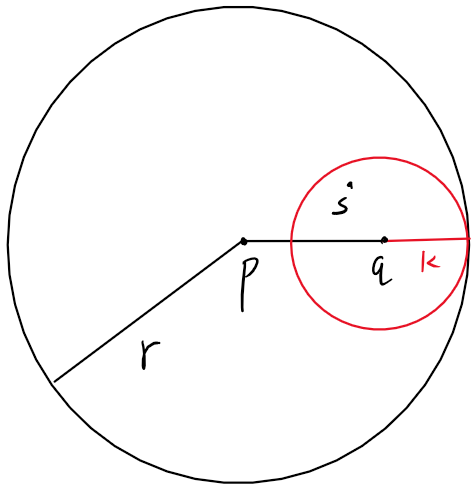
\includegraphics[scale=0.5]{linyushikaiji.png}
  \end{figure}

  \subsection{开集的补集}
  %相对开集与相对闭集
  $\forall E\subseteq X:$
  $$
  E^C\text{是闭集}\leftrightarrow E\text{是开集}
  $$
  \subsubsection{Démonstration}
  \subsubsection{Proposition}
  同理,补集是开集的集合是闭集.
  \subsection{Proposition: 开集的无限并与并集的无限交}
  $$
  \forall \alpha ,U_\alpha\text{是开集}\Rightarrow\bigcup_\alpha U_\alpha\text{是开集}
  $$
  $$
  \forall \beta ,E_\beta\text{是闭集}\Rightarrow\bigcap_\beta U_\beta\text{是闭集}
  $$
  \subsection{Proposition: 开集的有限交与并集的有限并}
  $$
  \forall \alpha ,U_\alpha\text{是开集}\Rightarrow\bigcup_\alpha U_\alpha\text{是开集}
  $$
  $$
  \forall \beta ,E_\beta\text{是闭集}\Rightarrow\bigcap_\beta U_\beta\text{是闭集}
  $$

  \subsection{闭包 L'adhérence}
  内点和极限点组成的几何叫做集合的闭包,记为$\overline{E}$即:
  $$
  \overline{E}=E\cup E'
  $$
  我们会给出一些关于闭包的简单的推论,它们都非常直观.
  \subsubsection{Exemple}
  $(114,514)$的闭包为$[114,514]$.
  \subsubsection{Remarque}
  闭包是闭集.
  \subsection{Proposition}
  与闭包相等的集合是闭集.
  $$
  E=\overline{E}\Leftrightarrow E\text{是闭集}
  $$
  \subsection{Proposition}
  集合$E$的闭包是包含它的最小闭集.
  \subsection{Proposition}
  对度量空间中的子集$E$,若:
  \begin{itemize}
    \item $E$有上界$\Rightarrow \sup E\in \overline{E}$
    \item $E$有下界$\Rightarrow \inf E\in \overline{E}$
  \end{itemize}
  \subsubsection{Démonstration}
  \noindent
  设$y=\sup E$.
  显然,若$y\in E$ 则$y\in \overline{E}$.\\
  若$y\notin E$ 则$\forall\epsilon>0\,\exists x\in E\, y-\epsilon<x<y $,也即$x\in N_\epsilon(y)\cap E$,则$y$是$E$极限点,故$y\in \overline{E}$.\
  $\inf$的证明一样.
  \subsubsection{Remarque}
  上述命题的逆命题不对.例如$[-114,0)\cup(0,514]$ 的上下界都属于该集合,但它不是闭集.
\section{相对开集/相对闭集}
  \subsubsection{Exemple}
  集合的开与闭受到其所在的度量空间的影响.设$E=(-3,3)$,则其在$\mathbb{R}$上是个开集,但是在$\mathbb{R}^2$上不是.
  这说明集合的开性质受到其所在度量空间的影响.为了消除这样的影响,我们需要讨论相对的开集和闭集.
  \subsection{相对开集}
  对度量空间$X$种的集合$E$和一点$q\in X$,若:
  $$
  \forall p\in E\,\exists r>0\,d(p,q)<r \Rightarrow q\in E
  $$
  则称$E$是$X$的相对开集.
  \subsection{Proposition}
  $Y\subseteq X\,,E\subseteq Y\,,G\in X$若$G$是开集,则:
  $$
  E=G\cap Y\Leftrightarrow E\text{是}Y\text{的相对开集}
  $$
  这个概念非常像\prettyref{myref:soustopo}提到的子空间拓扑.
  一个大空间里某个集合的性质仍属于这个集合和一个小空间交出来的集合.
  \subsection{相对闭集}
  对度量空间$X$种的集合$E$和一点$p\in X$,若:
  $$
  \forall p\in X\, \exists r>0\, N_r(p)\cap E\neq \varnothing\land N_r(p)\cap E\neq\{p\}\Rightarrow p\in E
  $$
  则称$E$是$X$的相对闭集.
  \section{紧集}%改到后面
    这部分内容放在这会显得很奇怪,因为在后面拓扑空间里我又会再讲一遍.
    但是为了Heine-Borel定理我又不得不讲清楚.
  \subsection{开覆盖}
  \subsubsection{有限子覆盖}
  \subsection{紧集}
  \subsection{相对紧致}
  \subsection{紧集的性质}
\section{Heine-Borel定理}
  \noindent
  OK,我们简单点,一上来我就把这个定理告诉你:\\
  对$E\subseteq \mathbb{R}^k\, k\in \mathbb{N}$,有:
  $$
  E\text{是紧集}\Leftrightarrow E\text{是闭集}\land E\text{是有界集}
  $$
  很显然,很直观,很一眼得出的结论.但是我们现在想要证明它可不简单.本节剩余的内容都是对这个重要定理的证明.
  \subsection{闭区间套性质}
  设$\mathbb{R}$中的一族闭区间$\{I_n \}\,, \forall n\in \mathbb{N}\,,I_n\subseteq I_{n+1}$,则有:
  $$
    \bigcap_{i=1}^\infty I_i\neq \varnothing
  $$
  闭区间套性质来源于$\mathbb{R}$的最小上界性.事实上这也是一种刻画实数集的方式,每个实数都是这样一族闭区间交集的极限.
  \subsubsection{Démonstration}
  证明非常简单,我已经给出了提示,就是最小上界性.设$I_i=[a_i,b_i]$,考虑闭区间下界组成的集合$E=\{a_i|i\in \mathbb{N}\}$,
  显然这个集合有上界(否则会得到$I_j=[a_j,b_j]\,b_j<a_j$),因此设最小上界$x=\sup E$.此外,$\forall i\in \mathbb{N}\,,b_i$也是$E$的上界,
  故有$x<b_i$,因此有$x\in[a_i.b_i]$.
  \subsection{$k$维格子}
  闭区间套性质不止是用于$\mathbb{R}$,而是可以类似地推广到$\mathbb{R}^k$.
  向量集
  $$\{\textbf{x}=(x_1,\dots,x_k)|x_j\in[a_j,b_j]_{j\in[\![1,k]\!]} \} $$
  称为$k$维格子.
  \subsubsection{Exemple}
  \begin{itemize}
    \item 1维格子就是上文提到的闭区间.
    \item 2维格子是一个封闭的矩形.
    \item 3维格子是一个长方体.
  \end{itemize}
  \subsection{$k$维格子的嵌套性质}
  设$\mathbb{R}^k$中的一族闭$k$维格子$\{I_n \}\,, \forall n\in \mathbb{N}\,,I_n\subseteq I_{n+1}$,则有:
  $$
    \bigcap_{i=1}^\infty I_i\neq \varnothing
  $$
  \subsubsection{Démonstration}
  这里的证明是闭区间套性质证明他推广,请读者自行尝试.只需要证明存在一组$x*=(x_1*,\dots,x_n*)$属于所有的$I_n$就行.

  \subsection{$k$维格子的紧致性}
  $k$维格子是紧集.
  \subsubsection{Démonstration}

  \subsection{Proposition}
  设$\mathbb{R}^k$中的子集$E$,则有:
  $$
  E\text{有界}\Leftrightarrow\exists I=\{\textbf{x}=(x_1,\dots,x_k)|x_j\in[a_j,b_j]_{j\in[\![1,k]\!]} \}\in \mathbb{R}^k\,, E\subseteq I
  $$
  \subsection{Heine-Borel定理}
  对$E\subseteq \mathbb{R}^k\, k\in \mathbb{N}$,有:
  $$
  E\text{是紧集}\Leftrightarrow E\text{是闭集}\land E\text{是有界集}
  $$
  \subsubsection{Démonstration}
  \noindent
  $\Rightarrow$:\\
  $\Leftarrow$:\\

  \subsection{实紧集的极限点}
  $\mathbb{R^k}$的子集$E$是紧集$\Leftrightarrow$$E$的每个无限子集在其中都有一个极限点.
  \subsubsection{Démonstration}
  \subsection{Weierstrass定理}

  \section{完备集与连通集}
  \subsection{Cantor三分集}
  \subsection{分离集}


  

\chapter{赋范空间\\Espace Vectoriel Normé}
  这一章的核心概念是范数(模)的推广。把以前所学习的范数抽象化,然后推广应用.
\section{范数 La norme}
  范数是映射,也是泛函。对于以前学习过的模长,我们发现其具有非负性、绝对齐次性和三角不等式三个优秀的性质,于是我们将其提取出来并推广,重新定义范数。
  \subsection{Définition}
  给定映射:
  $$
  \Vert \cdot \Vert : \mathbb{E} \longrightarrow \mathbb{R}
  $$
  满足:\\
  1.非负性:$\forall\alpha\in\mathbb{E}, \Vert \alpha \Vert\ge0$并且$\forall\alpha=0\Leftrightarrow \alpha=0_\mathbb{E}$。\\
  2.绝对齐次性(homogénéité):$\forall\alpha\in\mathbb{E}, \Vert k\alpha \Vert=| k | \Vert \alpha \Vert$。这里$k$属于$\mathbb{R}$或者$\mathbb{C}$,具体由$\alpha$决定。\\
  3.三角不等式(inégalité triangulaire):$\forall(\alpha,\beta)\in\mathbb{E}^2, \Vert \alpha+\beta \Vert\leq\Vert \alpha \Vert+\Vert \beta \Vert$。\\
  即可称该映射是一个范数,并称$(\mathbb{E},N)$为一个赋范向量空间(sspace vectoriel normé)
  ,简称赋范空间,其中N为范数。
  \subsection{Remarque:线性}
  所谓齐次性,指的是$f(k\alpha)=kf(\alpha)$,绝对齐次性就是$f(k\alpha)= | k | f(\alpha)$。另外还有可加性$f(\alpha+\beta)=f(\alpha)+f(\beta)$。
  同时满足齐次性和可加性的运算称线性。为了明确乘法和加法,范数的公理化必须在线性空间内。
  \subsection{Proposition:范数诱导的度量}
  \subsection{平移不变性}


\section{$L^P$范数}\label{myref:LPnorme}
与讲义上的顺序不同,我打算直接定义$L^P$范数(又称为$P$范数)并研究它的性质,而不是通过需要的性质去定义三个范数。
  \subsection{Définition}
  对线性空间里的向量$\alpha=(a_1,a_2,\dots,a_n$),定义范数:
  $$
    \Vert \alpha\Vert_P=(\sum_{i=1}^{n}|a_i|^P)^{\frac{1}{P}},P\ge1  
  $$
  容易验证$L^P$范数的非负性和绝对齐次性,其三角不等式由Minkowski不等式得出。\\
  当$P=1$,$L^1$范数称曼哈顿(Manhattan)范数,诱导的度量称曼哈顿距离。这是因为曼哈顿的街道都建得方方正正,从街道上一点到另一点的距离基本上就是走出两条垂直的线的长度。\\
  当$P=2$,$L^2$范数称即是通常意义下的范数,诱导的也就是通常意义下的距离\\
  当$P\rightarrow \infty$,$L^\infty$范数称一致范数(或者上确界范数),诱导的度量称切比雪夫(Chebyshev)距离,又叫棋盘距离。两点之间的距离是其各个坐标数值中绝对值最大的那一个。
  显然,这是因为$\Vert \alpha\Vert_\infty=\max\{|a_i|\}$\\
  当$P<1$时,Minkowski不等式不成立,需要反号,无法定义范数,但仍然有许多有趣的性质。
  \subsection{开球 La boule ouverte}
  \subsubsection{Définition}
  赋范空间$(E,\Vert \cdot \Vert)$中,有$q\in E,r\in(0,+\infty)$,对于集合:
  $$
    B(q,r)=\{x\in E |\Vert x-q \Vert<r \}
  $$
  称$B$是以$q$为中兴半径$r$的开球。请对照\prettyref{myref:voisinage},开球与邻域的区别,其实就是度量和范数的差异。
  \subsection{单位球与等距线}
  称$B(0,1)$为赋范空间$(E,\Vert \cdot \Vert)$上的单位球(boule unité)。作距离为1的各范数的等距线:
  \begin{figure}[H]%插入题目的图片
    \centering
    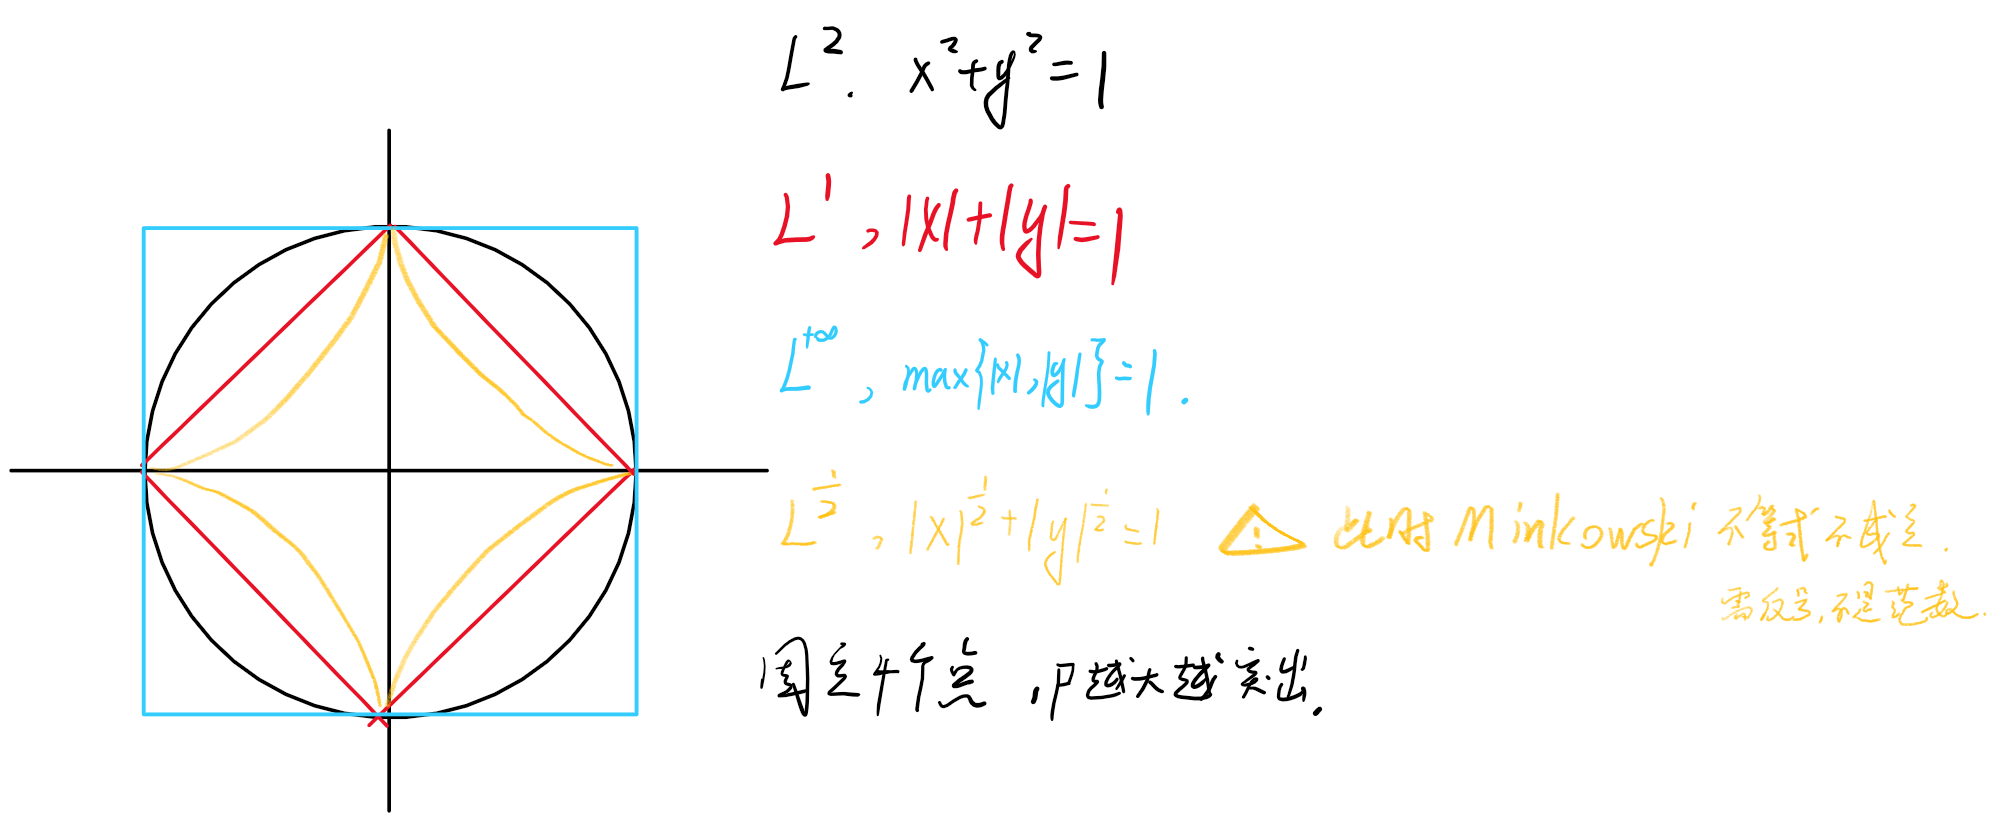
\includegraphics[scale=0.6]{danweiqiu.png}
    \label{fig:1}
  \end{figure}
  特别说明,我这里给出了$P=\frac{1}{2}$的情况,用来说明,对于单位球,其实就是固定4个点,然后P越大曲线越往外凸。
  \subsection{函数空间上的$L^P$范数}
  既然有了Euclide空间上的$L^P$范数,我们自然也会想在其他空间上玩玩这个。最熟悉的空间莫过于函数空间了!
  仿照之前的$L^P$范数,我们发现,不太好给函数又加和又开方什么的。但是所幸我们有一个替代方案,那就是同样非常熟悉的Riemann积分!
  \subsubsection{Définition}
  对$\mathcal{C} ^0I$上的函数$f$,定义范数:
  $$
  \Vert f \Vert_P=(\int_{I}|f(x)|^P \mathrm{d} x)^{\frac{1}{P}},P\ge1
  $$
  这样就得到了函数空间上的$L^P$范数!
  \subsubsection{Remarque}
  我们发现,当$P\rightarrow \infty$时$L^\infty$范数$\Vert f \Vert_\infty=\max|f(x)|,x\in I$,这正是函数$f$在$I$上的上确界。
  现在回顾之前我们对一致收敛的定义,那里提到的$\Vert f_n-f \Vert_\infty\rightarrow 0$就非常好理解了。
\section{空间的完备化}
  \subsection{实数:七个等价命题}
  \subsection{收敛}
  当我们尝试把范数、度量、内积等等概念都抽象化、公理化地定义了之后,是时候重新回顾一下,一个重要概念——收敛了。当然,课程的内容只在赋范空间内讨论了收敛,所以我们先看赋范空间内的。
  我们会尝试用精确的$\epsilon-\delta$语言来定义它:
  \subsubsection{Définition}
  赋范空间$(E,\Vert \cdot \Vert)$中,点列$(u_n)_{n\in\mathbb{N}},l\in E$,若:
  $$
    \forall\epsilon>0, \exists p\in \mathbb{N}, n\ge p\Rightarrow \Vert u_n-l \Vert<\epsilon
  $$
  称$(u_n)_{n\in\mathbb{N}}$在$(E,\Vert \cdot \Vert)$中收敛于$l$。
  \subsection{Proposition}
  若$(u_n)_{n\in\mathbb{N}}$在$(E,\Vert \cdot \Vert)$中收敛于$l$,则$(u_n-l)_{n\in\mathbb{N}}$在$(E,\Vert \cdot \Vert)$中收敛于$0$。
  \subsection{Proposition}
  若$(u_n)_{n\in\mathbb{N}}$在$(E,\Vert \cdot \Vert)$中收敛于$l_1$和$l_2$,且二者同属于赋范空间$(E,\Vert \cdot \Vert)$,则$l_1=l_2$
  
  
  \subsection{Cauchy列与收敛}
  \subsubsection{Définition}
  度量空间$(X,d)$中,点列$(u_n)_{n\in\mathbb{N}}$,若:
  $$
    \forall\epsilon>0, \exists p\in \mathbb{N}, m>p,n>p\Rightarrow d(u_m,u_n)<\epsilon
  $$
  称点列$(u_n)_{n\in\mathbb{N}}$是一个Cauchy列。
  \subsubsection{Proposition}
  度量空间中收敛的点列一定是Cauchy列。
  \subsubsection{Proposition}
  度量空间中的Cauchy列一定有界。
  \subsubsection{Proposition}
  子列收敛的Cauchy列一定收敛。


  \subsection{再论闭包与稠密集}
  \subsubsection{闭包}
  现在我们可以尝试把集合拖到赋范空间里,尝试定义集合的闭包。
  对赋范空间$(E,\Vert \cdot \Vert)$中的集合$A$,定义其闭包为:
  $$
    \overline{A}=\{x\in E | \forall(a_n)\in A^\mathbb{N},a_n\xrightarrow[n\rightarrow+\infty]{}x\}
  $$

  \subsubsection{Proposition}
  赋范空间$(E,\Vert \cdot \Vert)$中的集合$A\in\overline{A}$。
  \subsubsection{稠密集}
  对赋范空间$(E,\Vert \cdot \Vert)$和其中的集合$A$,如果:
  $$
    \forall x\in E, \exists (a_n)\in A^\mathbb{N}, a_n\xrightarrow[n\rightarrow+\infty]{}x
  $$
  称集合$A$在$E$上是稠密的。显然,常见的如有理数集在实数集上仍然是稠密的。
  \subsubsection{Bonus}
  Pierre曾在某次作业里要求证明无理数集在$\mathbb{R}$上稠密。当你学了这里的定义之后应该就非常简单了。当时我是这么写的:\\

    Soit $\mathbb{I} =\mathbb{R}\setminus \mathbb{Q}$.
    $\forall x\in \mathbb{R}$:\\
    \indent
    Si $x\in \mathbb{I}$, 
    soit une suit $\left \{ \alpha_n \right \}=x \Rightarrow 
    \lim_{n \to \infty}x=x\in \mathbb{\overline{I}}$.\\
    \indent
    Si $x\in \mathbb{Q}$, 
    soit une suit $\left \{ \beta_n \right \}=x-\frac{\sqrt{2}}{n}$. 
    $\forall n\in \mathbb{N}, \beta_n=x-\frac{\sqrt{2}}{n}\in \mathbb{I}$ et 
    $\lim_{n \to \infty}\beta_n=x\in \mathbb{\overline{I}}$.\\
    \indent
    Donc $\forall x\in \mathbb{R}, \exists (a_n)_{n\in\mathbb{N}}\in \mathbb{I}^{\mathbb{N}}, n\xrightarrow[a_n\rightarrow\infty]{}x$. 
    Cela dit que $\mathbb{I}=\mathbb{R}\setminus \mathbb{Q}$ est dense dans $\mathbb{R}$.\\


  \subsection{完备空间与完备化}
  \subsubsection{Définition}
  若度量空间$(X,d)$中任意一个Cauchy列都收敛,称度量空间$(X,d)$是完备的(complet)度量空间。
  称完备的赋范空间为Banach空间,完备的内积空间为Hilbert空间。想要熟悉这两个空间的具体性质就去学习泛函分析吧。\\

  把一个度量空间加上其Cauchy列的极限点组成的最小度量空间这一过程称为对度量空间的完备化。例如,有理数集的完备化就是实数集。

\section{等价度量与等价范数}  \label{myref:normeq}
  \subsection{双Lipschitz条件}
  给定两个度量空间$(E_1,d_1),(E_2,d_2)$,集合$U\subseteq E_1$。
  若对于函数$f:U\rightarrow E_2$存在常数$K$使得对任意集合$U$中的元素$(a,b)$有:
  $$
  d_2(f(a),f(b))\leq Kd_1(a,b)
  $$
  称该函数符合Lipschitz条件。\\
  若存在$K\ge 1$使得:
  $$
  \frac{1}{K}d_1(a,b)\leq d_2(f(a),f(b))\leq Kd_1(a,b)
  $$
  称该函数符合双Lipschitz条件。
  \subsection{等价范数 La norme équivalente}
  \subsubsection{Définition}
  设线性空间$E$上的两个范数$N_1$和$N_2$若:
  $$
    \exists(a,b)\in(0,+\infty),\forall x\in E,aN_1(x)\leq N_2(x)\leq bN_1(x)
  $$称$N_1$和$N_2$是等价(équivalente)范数。
  \subsubsection{Remarque}
  等价范数是等价关系,具有自反性、传递性和对称性。
  \subsubsection{Proposition}
  n维线性空间上的所有范数等价。

\chapter{内积 Produit Scalaire}
  这一部分是在小学期讲的。
    \subsection{Définition}
    \subsection{Cauchy-Schwatz不等式}
    \subsection{内积诱导的范数}
    \subsection{平行四边形等式}


\chapter{拓扑入门\\Introduction:La Topologie}
拓扑是什么?拓扑学内容有哪些?拓扑这个词或许经常听到,但是对于具体的含义和内容想必不是很了解。
事实上,从度量开始,就已经可以算是拓扑学的内容了,我们已经学习了好几章的拓扑学,只不过到了这一章才正式地把这些概念定义出来。
之前我们完成了距离的公理化、模长的公理化和内积的公理化,拓扑也是一个我们熟悉的概念公理化,那就是开集。
拓扑研究的就是开集的集族(Famille d'ensembles)。
\section{拓扑空间}
  与度量空间、赋范空间和内积空间类似,拓扑也有对应的拓扑空间,定义如下:
  \subsection{Définition}
  给定集合$X$和集族$\tau $,满足:
  $$
  \begin{aligned}&
  1.\varnothing\in\tau , X\in\tau\text{,空集和全集是开集}\\&
  2.\forall\alpha\in I,U_\alpha\in\tau \Rightarrow\bigcup_{\alpha\in I}U_\alpha\in\tau \text{,开集的并集是开集。}\\&
  3.\forall n\in\mathbb{N},\bigcap_{i=1}^{n}U_i\in\tau \text{,开集的有限交是开集。}\\
    \end{aligned}
  $$
  则称$\tau $是$X$上的一个拓扑,称$(X,\tau)$是一个拓扑空间,$U$称其中的开集。
  \subsection{Remarque:其他的公理化}
  除了以上的公理化方式,还有两种常见的拓扑定义。
  \subsection{Proposition:闭集}
  由de Morgan定律得:
  $$
  \begin{aligned}&
  1.\varnothing, X{ 是闭集。}\\&
  2.\forall\alpha\in I,E_\alpha\text{是闭集} \Rightarrow\bigcap_{\alpha\in I}E_\alpha \text{是闭集。闭集的交是闭集。}\\&
  3.\forall n\in\mathbb{N},\bigcup_{i=1}^{n}E_i \text{是闭集。闭集的有限并是闭集。}\\
    \end{aligned}
  $$
  \subsection{Exemple}
  $\mathbb{R}$上的所有形如$[a,b)$的区间可以组成一个拓扑,其中每个$[a_i,b_i)$都是开集。

  \subsection{离散拓扑 Topologie discrète}
  离散拓扑即$\tau=\mathcal{P} (X)$,其拓扑是集合的幂集,也就是其所有子集的集族。
  离散拓扑空间里所有的单点集都既是开集又是闭集,相互之间都是"孤立的"。

  \subsection{密着拓扑 Topologie grossiète}
  密着拓扑即$\tau=\{X,\varnothing \}$,又叫不可分拓扑,其空间里只有空集和整个空间是开集,所有的点都被"粘在一起",无法通过拓扑的方式区分开来。\\
  
  可以认为,离散拓扑和密着拓扑是两个"极端的"拓扑,全包和全不包。
  也正因为其极端性,它们有着一些特殊的性质,我们在后续研究。
  
  \subsection{度量诱导的拓扑}
  对$(X,\tau)$,若存在度量$d$可以定义拓扑的开集,称$(X,\tau)$是可度量的(英:metrizable)。
  例如,\prettyref{myref:lisanduliang}的离散度量可以诱导离散拓扑,此时邻域$N_\frac{1}{2}=\{X\}$就是开集。
  而对于card$(X)>1$的密着拓扑就无法被度量。
  \subsection{有限补拓扑 Topologie des compléments finis}
  有限补拓扑中,补集有限的集合是开集。即$\tau=\{U|U\subseteq X,U^C\text{是有限集} \}\cup \{\varnothing\}$

  \subsection{子空间拓扑}\label{myref:soustopo}
  提前预告一下,这是个简单但是非常重要的概念,我们在后面的证明中会多次用到这个概念。\\
  对$(X,\tau)$,$Y$是$X$的子集,则存在一个拓扑$\tau_y=\{Y\cap U| U\in\tau\}$,也就是说,拓扑与子集的交集可以组成一个新的拓扑。
  \subsubsection{Démonstration}
  $$
  \begin{aligned}&
  \varnothing\cap Y=\varnothing\in\tau_y\\&
  X\cap Y=Y\in\tau_y\\&
  \bigcup_{\alpha\in I}(U_\alpha\cap Y)=(\bigcup_{\alpha\in I}U_\alpha)\cap Y\in Y\\&
  \bigcap^n_{i=1}(U_i\cap Y)=( \bigcap^n_{i=1}U_i)\cap Y\in Y
  \end{aligned}
  $$
  \subsubsection{Exemple}
  对于$\mathbb{R}$上的常规拓扑和子集$Y=[0,+\infty),\forall (a,b)\in\mathbb{R},(a,b)\cap[0,\infty)\in\tau_y$.
\section{拓扑空间里的点集}
  现在让我们来看一看那些以前很熟悉的概念拿到拓扑空间里之后会发生什么.
  \subsection{邻域}
  对$(X,\tau)$中的一点$x$,若存在开集$U\in\tau, x\in U$,则称$U$是$x$的一个邻域,记为$U(x)$,$U/x$是$x$的去心邻域,记为$\check{U}(x) $.
  细心的读者可能会发现,现在的邻域跟之前的在对称性上有所差异,之前我们规定一个点的邻域好像都是关于这个点"对称"的,点在邻域的正中央,现在这个点可以在邻域里的任意位置。
  我当初学到这里也觉得奇怪,但是后面一想,也没用上这个所谓的对称性啊,所以其实问题不大.
  \subsection{内点}
  $(X,\tau), E\subseteq X,x\in E,\text{若存在} U(x)\subseteq E$则称呼$x$是$E$的一个内点. $E$的所有内点组成的集合称为其内部,记为$E^O$.
  \subsection{极限点与闭包点}
  $(X,\tau), E\subseteq X,x\in E$若有$\forall\check{U}(x)\cap E\neq\varnothing$,则$x$是$E$的极限点.$E$的所有极限点组成的集合称为导集,记为$E'$.同理,
  若有$\forall U(x)\cap E\neq\varnothing$,则$x$是$E$的闭包点.$E$的所有闭包点组成的集合称为闭包,记为$\bar{E}$.
  熟悉的感觉又回来了.同样,我们可以证明$\bar{E}=E\cup E'$.
  \subsection{外点与边界点}
  与内点这个概念相对应,考虑$E$的补集$E^C$,将其内点称为$E$的外点,组成的集合称为外部,记为$E^e$.不是内点又不是外点的点称为边界点,组成的集合称为边界,记为$\partial E$.
  \subsection{熟悉的命题}
  把以前的一些命题拿过来放到拓扑空间,它们仍然成立.
  \begin{itemize}
    \item $U\text{是开集}\Leftrightarrow U=U^O$,内部等于自身的集合是开集.
    \item $U^O=(U^O)^O$,内部是开集.
    \item $U^O$是包含于$U$的最大开集.
    \item $E\text{是闭集}\Leftrightarrow E=\bar{E}$,闭包等于自身的集合是闭集.
    \item $\bar{E}=\bar{\bar{E}}$,闭包是闭集.
    \item $\bar{E}$是包含于$E$的最小闭集.
  \end{itemize}
  \subsubsection{Démonstration}
  待补充,笔记上的太乱了.



\section{拓扑空间里的收敛}
  现在我们要在拓扑空间中再次研究这个重要的,贯穿了大量分析学内容的概念————收敛.
  \subsection{Définition}
  $(X,\tau)$中的点列$\{a_n\}$和一点$x$,若有:
  $$
  \forall U(x), \exists N\in \mathbb{N}*\text{使得}n>N\Rightarrow a_n\in U(x)
  $$
  称点列$\{a_n\}$收敛于点$x$.
  \subsubsection{Exemple}
  $X=\{a,b,c\},\tau =\{\varnothing, X, \{a,b\}, \{a,c\}, \{a\}\},a_n\equiv a$.则有$\{a_n\}$收敛于点$a$.
  \subsubsection{Remarque:收敛不唯一}
  注意到,在上述的条件里,点列的收敛是不唯一的!!!因为$\{a,b\}$也是点$a$的邻域,所以$\{a_n\}$收敛于点$b$;$\{a,c\}$也是点$a$的邻域,所以$\{a_n\}$收敛于点$c$.也就是说,$\{a_n\}$同时收敛于$a,b,c$三个不同的点!
  这多么可怕,与我们之前见过的只收敛到一个点的收敛概念完全不同.出现这一情况,是因为在之前我们学习的空间里,两个点之间存在没有交集的邻域,但是在拓扑空间里这条法则失效了,所以收敛有了这样的奇怪的性质.
  然而这不是什么好的性质,如果点列的收敛是不唯一的,那我们就无法区分收敛到的哪些点了,点集拓扑的探讨也就失去了意义.
  所以这一个收敛的定义其实不重要,因为没什么用.我们必须对它加以改进,添加更多的限制条件来确保能有效运用收敛.
  \subsection{Hausdorff条件:$T_2$公理}
  对$(X,\tau)$中任意两点$x_1,x_2$,若:
  $$
    \forall(x_1,x_2)\in X^2, x_1\neq x_2, \exists U(x_1),U(x_2)\text{使得}U(x_1)\cap U(x_2)=\varnothing
  $$
  则称$X$是一个Hausdorff空间.该条件又称为拓扑空间里的分离公理,或者$T_2$公理,它把空间里的点分离开了.
  \subsubsection{Proposition}
  一个有限集是一个Hausdorff空间,当且仅当它的$\tau$是离散拓扑.
  \subsubsection{Démonstration}
  离散拓扑的有限集显然是Hausdorff空间.我们证明另一个方向,利用反证法:
  $$
  \begin{aligned}&
    \lnot (\tau\text{是离散拓扑})\Rightarrow \exists x\in X, \{x\}\notin \tau\\&
    \text{设}x \text{的所有邻域交集为}\mathbb{U}\Rightarrow\mathbb{U}\cap x\neq\varnothing \\&
    \text{设}y\in\mathbb{U}\cap x\\&
    \Rightarrow \forall U(y)\cap\mathbb{U}\neq\varnothing\\&
    \Rightarrow \forall U(y),\forall U(x),U(y)\cap U(x)\neq\varnothing\\&
    \Rightarrow X\text{不是Hausdorff空间}
    \end{aligned}
  $$
  所以我们发现,如果研究有限集,那就绕不开离散拓扑,研究其收敛性也就没什么意义了.
  \subsubsection{Proposition}
  Hausdorff空间里点列的收敛具有唯一性,即$\{a_n\}$收敛于点$x$和$y\Rightarrow x=y$.
  \subsection{Hausdorff空间里的闭集}
  Hausdorff空间里单点集都是闭集.
  \subsubsection{Démonstration}
  对于Hausdorff空间里一点$x$,有:
  $$
  \forall y\in x^C, \exists U(y)\cap x\neq\varnothing\Rightarrow U(u)\subseteq x^C\Rightarrow y\in(x^C)^O
  $$因此$x^C$是个开集,那$x$自然就是个闭集了.
  \subsubsection{Proposition}
  Hausdorff空间里有限集都是闭集.
  \subsubsection{Proposition}
  度量空间都是Hausdorff空间.

  \subsection{Fréchet条件:$T_1$公理}
  在证明Hausdorff空间里单点集都是闭集的时候,我们用到了这样一步:
  $$
  \exists U(y)\cap x\neq\varnothing
  $$
  对比Hausdorff条件本身,我们发现这里没有用全.我们只用了点和邻域的关系而不是邻域和邻域的关系,这说明Hausdorff条件是一个很强的条件,我们可以尝试再稍微弱化一下它.
  于是就有了Fréchet条件:单点集都是闭集的拓扑空间称为Fréchet空间.





  \subsection{$T_0$公理与Kolmogorov体系}

\section{连续性与映射}
  现在,我们继续公理化拓扑空间里映射的连续性.
  \subsection{Définition}
  考虑两个拓扑空间$(X,\tau_x)(Y,\tau_y)$上的映射$f:X\rightarrow Y$,若:
  $$
  \forall U\in\tau_y,f_{-1}(U)\in\tau_x
  $$
  则称映射$f$是连续的.
  \subsection{拓扑的选择与连续性}
  对于同一个集合,我们选择不同的拓扑,则可能导致连续性的改变.
  例如,设$\mathbb{R}_d$是$\mathbb{R}$上的离散拓扑,$\mathbb{R}_n$是$\mathbb{R}$上的通常拓扑,$f(x)=x$是恒等映射,则:
  \begin{itemize}
    \item $f:\mathbb{R}_n\rightarrow \mathbb{R}_d$不是连续映射,单点集在$\mathbb{R}_n$上不是开集.
    \item $f:\mathbb{R}_d\rightarrow \mathbb{R}_n$是连续映射.
  \end{itemize}
  \subsection{由公理推导而来的等价命题}
  一下命题等价,它们分别对应着不同的拓扑公理.这也说明拓扑公理是可以相互转化的.
  \begin{itemize}
    \item 1.$\forall U\in\tau_y,f_{-1}(U)\in\tau_x$.(开集公理)
    \item 2.$\forall E\subseteq X,f(\bar{E})\subseteq \bar{f(E)}$.(闭包公理)
    \item 3.$\forall E\in Y\text{是闭集},f_{-1}(E)\in X\text{是闭集}$.(闭集公理)
    \item 4.$\forall x\in X, \forall U[f(x)], \exists U(x)\text{使得}f[U(x)]\subseteq U[f(x)]$.(邻域公理)
  \end{itemize}
  \subsubsection{Démonstration}
  $1\Rightarrow 2$:
  $$
  \begin{aligned}&
    \forall x\in \bar{E},f^{-1}U[f(X)]\cap E\neq\varnothing\\&
    \Rightarrow U[f(x)]\cap f(E)\neq\varnothing\Rightarrow f(x)\in \bar{f(E)}
    \end{aligned}
  $$


  $2\Rightarrow 3$:
  $$
  \begin{aligned}&
    \forall x\in \bar{f^{-1}(E)},f(x)\in \bar{E}\\&
    \Rightarrow x\in f^{-1}(E)\Rightarrow\bar{f^{-1}(E)}\subseteq f^{-1}(E)\\&
    \Rightarrow f^{-1}(E)\text{是闭集}
    \end{aligned}
  $$


  $3\Rightarrow 1$:
  $$
  \begin{aligned}&
    U\subseteq \tau_y\Rightarrow U^C\text{是闭集}\Rightarrow f^{-1}(U^C)\text{是闭集}\\&
    \Rightarrow f^{-1}(U^C)=[f^{-1}(U)]^C\Rightarrow f^{-1}(U)\in\tau_x
    \end{aligned}
  $$


  $4\Rightarrow 1$:
  这里的证明其实就是前面证明过的东西反过来,留给读者完成.
  \subsection{Exemple}
  接下来给出几个连续映射
  \subsubsection{常值映射}
  $$
    f:X\rightarrow  Y
  $$
  $$
    x\rightarrow C
  $$
  $\forall \text{开集}U\subseteq Y,C\in U\Rightarrow f^{-1}(U)=X \text{是开集}, 
  C\notin U\Rightarrow f^{-1}(U)=\varnothing \text{是开集}$,故常值映射是连续映射.
  \subsubsection{包含映射}
  包含映射是$X$的子集$A$上的恒等映射
  $$
    i:A\hookrightarrow  X
  $$
  $$
    x\rightarrow x
  $$
  $\forall \text{开集}U\subseteq X,i^{-1}(U)=U\cap A \text{是开集(子空间拓扑)}$,故常值映射是连续映射.
  \subsubsection{复合映射}
  给定连续映射$f:X\rightarrow  Y\text{    }g:Y\rightarrow  Z$,其复合映射
  $$
    \phi:X\rightarrow Z
  $$
  $$
    x\rightarrow g(f(x))
  $$
  也是连续映射.$\forall \text{开集}U\subseteq Z,g^{-1}(U)\subseteq Y 
  \text{是开集}\Rightarrow f^{-1}(g^{-1}(U))\subseteq X\text{是开集}\Rightarrow (f\circ g)^{-1}(U)\text{是开集}$,
  故连续映射的复合映射也是连续映射.
  \subsubsection{限制映射}
  考虑连续映射$f:X\rightarrow Y$,对$A\subseteq X:$
  $$
  f|_A:A\rightarrow Y
  $$
  $$
    x\rightarrow f(x)
  $$
  为连续映射(考虑包含映射和映射$f$的复合映射即可).
  \subsubsection{陪域缩小}
  考虑连续映射$f:X\rightarrow Y$,对$Z\subseteq X:$
  $$
    f': X\rightarrow Z
  $$
  $$
    x\rightarrow f(x)
  $$
  则$f'$也是连续映射(考虑映射$f$和包含映射的逆映射的复合映射即可).
  \subsubsection{陪域扩大}
  考虑连续映射$f:X\rightarrow Y$,对$Y\subseteq Z:$
  $$
    f': X\rightarrow Z
  $$
  $$
    x\rightarrow f(x)
  $$
  则$f'$也是连续映射(考虑映射$f$和包含映射的复合映射即可).
  \subsection{局部表示与粘接原理}
  在讨论拓扑空间上的连续函数时,我们不必要求直观地看出整个函数都是连续的,而是可以间接地"拼凑"出一个连续函数.
  若我们采用开集"拼凑",则这个过程称为连续性的局部表示;若采用闭集,则称为粘接原理.即对拓扑空间上的函数$f:X\rightarrow Y$:
  $$
    X=\bigcup_{\alpha\in I}U_\alpha ,\forall \alpha\in I, U_\aleph\text{是开集}
  $$
  $$
  \forall \alpha\in I,f|_{U_\alpha}:U_\alpha\rightarrow Y\text{连续}\Rightarrow f:X\rightarrow Y\text{连续}
  $$
  即为连续性的局部表示;
  $$
    X=\bigcap_{i=0}^{n}V_i ,\forall i\in[\![0,n]\!], V_i\text{是闭集}
  $$
  $$
    \forall i\in[\![0,n]\!],f|_{V_i}:V_i\rightarrow Y\text{连续}\Rightarrow f:X\rightarrow Y\text{连续}
  $$
  \subsubsection{Démonstration}
  \begin{figure}[H]%插入题目的图片
    \centering
    
\includegraphics[scale=0.2]{proofforreader.jpg}
  \end{figure}


\section{同胚 Homeomorphisme}
  现在我们来到了拓扑里面最重要的概念——同胚.你可能听过这个著名的笑话:\\

  一个拓扑学家把咖啡倒进了甜甜圈里.有人问他为什么不把咖啡倒进咖啡杯里,拓扑学家非常惊讶:"它们有什么区别?不是同胚的吗?"
  \subsection{Définition}
  对拓扑空间上的映射$f:X\rightarrow Y$若$f$满足:
  \begin{itemize}
    \item $f$是双射
    \item $f$是连续映射
    \item $f^{-1}$是连续映射
  \end{itemize}
  则称$f$是$X$到$Y$上的一个同胚映射,此时$X$和$Y$是同胚的.显然,同胚是一个等价关系.
  \subsection{Exemple}
  \subsection{Remarque}
  请回顾我们在\prettyref{myref:Homomorphisme}和\prettyref{myref:Isomorphisme}里提到的同态和同构,它们有什么相似的地方?\\

  在拓扑空间上前两条无法推出第三条性质,我们讲马上给出一个经典的反例用来说明这一点.
  \subsection{Exemple: 反例}
  给出由半开半闭区间$[0,1)$到单位圆上的映射
  $$
  f:[0,1)\rightarrow \{(x,y)|x^2+y^2=1\}
  $$
  $$
  x\mapsto\cos(2\pi x)+\sin(2\pi x)
  $$
  $f$是连续的双射,但是$f^{-1}$在$(1,0)$处不连续.
  这是因为我们把区间的两端"粘贴"了起来,这导致了拓扑性质的改变,因此无法保持同胚.事实上,只要进行了类似"粘贴""裁剪"或者"穿孔"等等操作,原来的拓扑就变了.
  这些操作会在拓扑学里严格定义,这里不再谈论.
  \subsection{Proposition}
  对$\mathbb{R}$上的一元函数$f:X\rightarrow Y$,有:$X,Y$是$\mathbb{R}$上的两个区间(不能是子集!).若:
  \begin{itemize}
    \item $f$是双射
    \item $f$是连续映射
  \end{itemize}
  则$X,Y$同胚.
  \subsection{Exemple: 反例}
  若上述推论里将\textbf{$X,Y$是$\mathbb{R}$上的两个区间} 改成 \textbf{$X,Y$是$\mathbb{R}$上的两个子集} ,则结论不成立.
  例如映射$f:X\rightarrow Y$有 $X=[0,1]\cup(2,3],Y-[0,2]$
  $$
  x\mapsto 
  \begin{cases}
    x &x\in[0,1]\\
    x-1 &x\in (2,3]
    \end{cases}
  $$
  则$f^{-1}$不连续.
  \subsection{Proposition}
  对双射$f:X\rightarrow Y$,若:
  $$
  U\text{是$X$上的开集}\Leftrightarrow f(U)\text{是$Y$上的开集}
  $$
  则$X,Y$同胚.

  \section{紧致性与列紧性}
  \subsection{拓扑不变量}
  与同构类似,同胚的拓扑空间也有一些不会变化或者相等的东西.这些东西被称为拓扑性质或者拓扑不变量.
  它们在同胚映射下保持不变.由于许多概念还没有讲到,我们仅仅给出拓扑不变量的概念,以便于大家理解拓扑空间上的紧致性.
  更多的拓扑不变量将在拓扑学中研究.
  \subsection{Remarque}
  我们将以前所学过的度量空间上的开覆盖推广到拓扑空间.这并没有难度,因为拓扑空间直接就是拿开集定义的,不需要额外添加什么内容.
  对拓扑空间$X$上的开集族$\{U_\alpha|\alpha\in I \}$满足
  $$
    X\subseteq \bigcup_{\alpha\in I}U_\alpha
  $$则称$\{U_\alpha\}$是拓扑空间$X$上的一个开覆盖.\\

  同理,若能找到一组有限个开集覆盖$X$,即A和B拥有相同的基数
  $$
  X\subseteq \bigcup_{i=1}^{n}U_i
  $$则称$\{U_\alpha\}$是拓扑空间$X$上的一个有限开覆盖/有限子覆盖.
  \subsection{Définition: 紧致}
  对拓扑空间$X$上的任意一个开覆盖,若都能找到一个有限子覆盖,则称$X$是一个紧致空间,或称$X$是紧的.
  若$Y\subseteq X$也是紧的,则称$Y$是一个紧致集/紧集.
  \subsection{Définition: 序列紧致}
  对拓扑空间$X$上的任意一个序列,若都能找到一个子序列$\{ x_n\}$收敛于$x\in X$,则称$X$是一个序列紧致空间,或称$X$是列紧的.
  若$Y\subseteq X$也是列紧的,则称$Y$是一个列紧集.
  \subsection{Remarque: }
  或许你还记得我们在度量空间上讨论的紧致性问题,当时我们并没有这么区分紧和列紧.
  事实上,在度量空间上,紧致性和列紧性是等价的,这两个概念都起源于Bolzano对于收敛子列的研究.
  在研究收敛性上,发展出了Bolzano-Weierstrass定理和Arzela-Ascoli定理等对于序列紧致性的结论;
  在研究连续性上,又发展出了Heine-Borel定理作为连续性的结论.
  早期的列紧性比紧致性更为直观(显然,度量下的点列收敛肯定比开集更加容易直观理解),因此Fréchet将现在的列紧性定义为紧致.
  但是后来随着拓扑空间研究的深入,人们发现两者不等价,且在拓扑空间上Heine-Borel利用开区间表示的紧致性更容易理解,更何况在一般的拓扑空间下无法讨论序列的收敛,
  因此最终由Pavel和Urysohn用Heine-Borel的方法定义紧致性,而将Bolzano-Weierstrass的方法定义为列紧性.在本章中,我们主要考虑紧致性的问题.
  \subsection{Proposition}
  $Y$是$X$上的一个紧致集等价于以下表述:
  $$
  \text{对开集族 }\{U_\alpha\}\subseteq X, \{U_\alpha\}\text{是 }Y\text{的开覆盖 }\Rightarrow
  \exists\{U_i|i\in[\![1,n]\!]\}\subseteq\{U_\alpha\}\text{是 }Y\text{的有限子覆盖 }
  $$
  这说明了一个很重要的结论:集合的紧致性与其在什么空间上无关.一个紧的$Y$放在任何$X$里都是紧的.
  \subsection{Exemple}
  \subsubsection{1.  $\mathbb{R}$既不紧,也不列紧}
  我们可以找到开覆盖
  $$
  C=\{(n,n+2)|n\in\mathbb{Z}\}
  $$
  从中拿去任意一个区间之后就无法覆盖$\mathbb{R}$了.\\
  对于$\mathbb{R}$趋近于正无穷的子列显然不收敛于$\mathbb{R}$上的某个点.
  \subsubsection{2.  $(0,1]$既不紧,也不列紧}
  \subsubsection{3.  $\{0\}\cup \{\frac{1}{n}|n\in\mathbb{N}\}$既紧,也列紧}
  \begin{figure}[H]%插入题目的图片
    \centering
    
\includegraphics[scale=0.2]{proofforreader.jpg}
  \end{figure}
  \subsection{紧集的投影}
  定义投影算子$\mathcal{P}:X^2\rightarrow X$
  $$
  (a,b)\mapsto a
  $$
  若$A^2$紧致,则$\mathcal{P}(A)$也紧致.
  \subsection{Proposition}
  两个紧集的笛卡尔积同样是紧集.
  $$
  A\times B\text{是紧集}\Leftrightarrow A\text{是紧集}\land B\text{是紧集}
  $$
  \subsection{Proposition}
  有限个紧集的笛卡尔积同样是紧集.(此时不能反推)
  $$
  A_1,\dots,A_n\text{是紧集}\Rightarrow A_1\times \dots\times A_n\text{是紧集}
  $$
  \section{闭集刻画的紧致集}
  利用闭集刻画紧致集,可以在一定程度上简化我们的计算和证明.
  \subsection{Remarque: 有限交性质}
  对集合$X$,设子集族$C=\{U_\alpha|\alpha\in I \}$,若对$C$的任一\textbf{有限}子集族$C_U=\{U_1,U_2,dots,U_n\}$,都有
  $$
  \bigcap_{i=1}^n U_i\neq \varnothing
  $$
  则称$C$具有\textbf{有限交性质}.
  \subsection{Proposition}
  \noindent
  $X$是紧集等价于以下陈述:\\
  对$X$中任意具有有限交性质的闭集族$\{V_\alpha|\alpha\in I\}$,有
  $$
    \bigcap_{\alpha\in I}V_\alpha\neq\varnothing
  $$
  \subsubsection{Démonstration}
  利用De Morgan定律和反证法.
   
  \subsection{Proposition}
  紧致空间内的任意闭子集都是紧集.
  \subsubsection{Démonstration}
  设$Y\subseteq X$,取$Y$的开覆盖$C=\{U_\alpha|\alpha\in I \}$,令$C'=C\cup Y^\complement$,
  则$C'$是$X$的一个开覆盖.若$X$是紧致的,设其有限子覆盖$D=\{U_1,U_2,dots,U_n\}\subseteq C'$.则有:
  $$
  Y^\complement\nsubseteq D\Rightarrow D\text{是}Y\text{的有限开覆盖}\Rightarrow Y\text{是紧集}
  $$
  $$
  Y^\complement\subseteq D\Rightarrow D\setminus Y^\complement \text{是}Y\text{的有限开覆盖}\Rightarrow Y\text{是紧集}
  $$
  \subsection{Proposition}
  Hausdorff空间里紧致集都是闭集
  \subsubsection{Démonstration}


  \subsubsection{Exemple: 反例}
  以上命题不可反推.例如考虑到非Hausdorff空间上$\mathbb{R}$的有限补拓扑,任意的闭集都是紧集,但是也是有限集.



\chapter{线性空间 \\Espace Vectoriel}
\chapter{矩阵的简化\\Reduction}

\section{特征值与特征向量 Vecteurs Propres et Valeurs Propres}
  在线性空间中,有一些有趣的线性变换(线性算子)和向量。这些向量经过这些变换前后都处在同一条直线上,仅仅是改变了长度或方向。
  能使向量拥有这种特质的线性变换往往也有许多优秀的性质可以研究,也就是本章的重点。\\
  
  对于这些经过变换前后都处在同一条直线上的向量,称其为对应线性变换的特征向量(le vecteur vropre),
  变换后改变的方向与大小所对应的标量称为线性变换的特征值(la valeur propre),
  将具有相同特征值的特征向量与一个同维数的零向量组成一个集合,称为线性变换的特征空间(l'espace propre).
  \subsection{Définition}
  设$n\in\mathbb{N} , M\in \mathcal{M}_n(\mathbb{K})$。
  若存在$x\in \mathcal{M}_{n,1}(\mathbb{K})\setminus\{0\}, \lambda\in\mathbb{K}$使得:
  \begin{equation}
    \notag
    Mx=\lambda x
  \end{equation}
  则称$\lambda$为矩阵$M$的特征值,$x$为矩阵$M$的特征向量,
  $E_\lambda=\{x\in\mathcal{M}_{n,1}(\mathbb{K})\}$为矩阵$M$的特征空间,
  称特征值集$\sigma_{\mathbb{K}}(M)$为矩阵$M$的谱(le spectre)。\\

  若$E$是域$\mathbb{K}$上的线性空间,自同态$u\in \mathcal{L} (E)$,同理
  若存在$x\in E\setminus\{0\}, \lambda\in\mathbb{K}$使得:
  \begin{equation}
    \notag
    u(x)=\lambda x
  \end{equation}
  则称$\lambda$为矩阵$M$的特征值,$x$为矩阵$M$的特征向量,
  $E_\lambda=\{x\in E\}$为矩阵$M$的特征空间,
  称特征值集$\sigma_{\mathbb{K}}(M)$为矩阵$M$的谱。事实上,如果$E$是有限维空间,两种定义是等价的。
  \subsubsection{Remarque}
  还记得\prettyref{myref:tezheng}介绍的“特征”的概念吗?想一下我们为什么要管这里的$\lambda$叫“特征”值.
  \subsection{Proposition:特征空间的性质}
  \subsubsection{线性子空间}
  $E_\lambda$是一个线性子空间(sous-espace vectoriel),满足:
  \begin{equation}
    \notag
    E_\lambda:
    \begin{cases}
    \lambda_i+\lambda_j\in E_\lambda \\
    m\lambda_i\in E_\lambda \\
    E_\lambda\neq \varnothing 
    \end{cases}
  \end{equation}
  \subsubsection{核空间}
  $E_\lambda$是$M-\lambda I_n$的核空间,即:
  \begin{equation}
    \notag
    E_\lambda=\ker(M-\lambda I_n)=\{x|(M-\lambda I_n)x=0_n\}
  \end{equation}
  \subsubsection{非零维度}
  根据特征空间的定义,其至少包含一个非0向量,故$\dim E_\lambda \ge 1$。


\section{特征多项式 Polynôme caractéristique}
  当我们知道了特征值和特征向量,自然就会想问:如何找到矩阵的特征值和特征向量呢?
  随机抽向量和数一个一个计算显然不可能。为了更加便捷,我们需要通过特征多项式来寻找特征值和特征向量。
  \subsection{Définition}
  设$n\in\mathbb{N} , M\in \mathcal{M}_n(\mathbb{K})$,有:
  \begin{equation}
    \notag
    \chi _M(X)=\det(XI_n-M)\footnote{
      需说明的是,许多教材里把特征多项式定义成$\det(M-XI_n)$,计算时需注意反号。两种形式并不影响各种结论。
    }
  \end{equation}
  称$\chi _M(X)$为矩阵$M$的特征多项式。
  显然,我们可以找到$\exists(a_0,...,a_{n-1})\in\mathbb{K}^n$使得:
  \begin{equation}
    \notag
    \chi _M(X)=X^n+\sum_{k=0}^{n-1}a_kX^k
  \end{equation}
  这就是一般的特征多项式的形式。并且,特征多项式的解即为矩阵的特征值。
  一般而言,对布于任何交换环上的方阵都能定义特征多项式。
  \subsubsection{Démonstration}
  \begin{equation}
    \notag
    \begin{aligned}
    & \chi _M(\lambda)=\det(\lambda I_n-M)=0\\
    & \Rightarrow \ker(M-\lambda I_n)\neq\{0\}\\
    & \Rightarrow (M-\lambda I_n)x=\{0\}\\
    & \Rightarrow \lambda\in\sigma_{\mathbb{K}}(M)\\
    \end{aligned}
  \end{equation}
  \subsection{Remarque:域上的特征值}
  在计算矩阵特征值时必须考虑域$\mathbb{K}$的限制。同一个矩阵在不同的域上可能有不同的谱。例如:
  $$
  \begin{aligned}
    R=\begin{pmatrix} 0 & -1 \\ 1 & 0 \end{pmatrix}\\
  \end{aligned}
  $$
  有特征多项式$\chi _R(X)=X^2-1$:\\
  若在实数域上$R\in \mathcal{M}_2(\mathbb{R})$则$\sigma_{\mathbb{R}}(R)=\varnothing$,\\
  若在实数域上$R\in \mathcal{M}_2(\mathbb{C})$则$\sigma_{\mathbb{C}}(R)=\{i,-i\}$。
  \subsection{二阶特征多项式}
  对二阶矩阵$\mathcal{M}_2(\mathbb{K})$,特征多项式可以简化为:
  $$
  \chi _R(X)=X^2-\mbox{tr}(M)X+\det(M)
  $$
  \subsection{秩为1的自同态}
  对自同态$u\in\mathcal{L} (\mathbb{R}^n)$,若$u$的秩为1,则特征多项式可以简化为:
  $$
  \chi _u(X)=X^{n-1}(X-\mbox{tr}(u))
  $$
  \subsection{多项式的分裂域}
  本节只对分裂域(根域)作简单介绍,详细内容过于复杂,不在本课程讨论范围内。
  在抽象代数中,一个系数域为$\mathbb {K}$ 的多项式${P(x)}$的分裂域(根域)是
  $\mathbb {K} $的“最小”的一个扩域$\mathbb{L}$,
  使得在其中$P(x)$可以被分解为一次因式$x-r_{i}$的乘积,
  其中的$r_{i}$是$\mathbb{L}$中元素。
  一个$\mathbb {K} $上的多项式并不一定只有一个分裂域,
  但它所有的分裂域都是同构的,也就是在同构意义上,$\mathbb {K} $上的多项式的分裂域是唯一的。
  \subsubsection{Définition}
  若存在$(c,\alpha_1,\dots,\alpha_n)\in\mathbb{K}^{n+1}$使得:
  $$
    P(X)=c\prod_{i=1}^{n} (X-\alpha_i)
  $$
  称$P$在$\mathbb {K} $上是分裂的(scindé)。这意味着$P$所有的根都在$\mathbb {K} $上。为了更好地理解分裂域,我们举几个例子:
  \subsubsection{Exemple 1}
  $$
    P(X)=(X^2-2)
  $$
  $P$在$\mathbb {R} $和$\mathbb {C} $上都可分裂成$P(X)=(X+\sqrt{2})(X-\sqrt{2})$。
  \subsubsection{Exemple 2}
  $$
    Q(X)=(X^2+4)
  $$
  $Q$在$\mathbb {C} $上可分裂成$Q(X)=(X+2i)(X-2i)$,但是在R上不可分裂。
  \subsection{代数重数La multiplicité}
  在一些地方可能会遇到如下的表示方法:"一个矩阵A的特征值为4,4,3,3,3,2,2,1。"
  事实上,我们可以直接得出A的特征值是\{4,3,2,1\},那为什么要对数字进行重复呢?
  根据特征多项式的解法,很容易猜测,重复的次数就是特征值作为根出现的次数,也即代数重数。
  \subsubsection{Définition}
  设多项式$P\in\mathbb {K} [X], \alpha\in\mathbb {K}$,若存在$Q\in\mathbb {K} [X]$使得
  $$
    P(X)=(X-\alpha)^mQ(X)\mbox{且}Q(\alpha)=\neq 0
  $$
  称$m$为根$\alpha$的代数重数。在特征多项式中,记特征值$\lambda$的代数重数为$\mu(\lambda)$。
  \subsubsection{Exemple 1}
  $$
  P(X)=(X-1)^{14}-(X-51)^4
  $$
  其中根1的代数重数为14,根51的代数重数为4。
\section{相似矩阵 Matrice semblable}
  \subsection{Définition}
  设$A$和$B$都属于域$\mathbb {K}$ 上的$n$阶方阵,即$\mathcal{M}_n(\mathbb{K})$。
  若存在$P\in\mathcal{G} \mathcal{L} _n\mathbb{K}$使得:
  $$
    A=PBP^{-1}
  $$
  称$A$和$B$是相似的(semblable)。易知相似是一种等价关系。
  \subsubsection{Remarque}
  嘿!还记得\prettyref{myref:conjugaison}提到的共轭关系吗?这就是共轭关系在矩阵里的应用!
  \subsection{Proposition:相似矩阵的特征多项式相等}
  设$A$和$B$是相似矩阵,$\chi_A(X)$和$\chi_B(X)$分别是他们的特征多项式,则有:
  $$
  \chi_A(X)=\chi_B(X)
  $$
  \subsubsection{Démonstration}
  $$
  \begin{aligned}
  &  \chi _A(X)=\det(XI_n-A)=\det(XI_n-PBP^{-1})=\det(XPI_nP^{-1}-PBP^{-1})\\
  &  =\det(P(XI_nP^{-1}-BP^{-1}))=\det(P(XI_n-B)P^{-1})\\
  &  =\det(P)\det(XI_n-B)\det(P^{-1})\\
  &  =\det(XI_n-B)=\chi _B(X)
    \end{aligned}
  $$
  \subsubsection{Proposition}
  若$A$和$B$是相似矩阵,则同理有$\sigma_{\mathbb{K}}(A)=\sigma_{\mathbb{K}}(B)$
  \subsection{Remarque:特征多项式相等不一定相似}
  
  \begin{equation}
    \notag
    A=\begin{pmatrix} 1 & 1 \\ 0 & 1 \end{pmatrix}
    B=\begin{pmatrix} 1 & 0 \\ 0 & 1 \end{pmatrix}
  \end{equation}
  两者的特征多项式都是$(X-1)^2$但明显二者无法相似转化。
  \subsection{Proposition}
  几何重数小于等于代数重数.
  称特征值$\lambda$对应特征空间$E_\lambda$的维数$\dim E_\lambda$为该特征值的几何重数,则有:
  $$
    \forall\lambda\in\sigma_{\mathbb{K}}(M), \dim E_\lambda\leq\mu\lambda
  $$


  如果将代数重数视为一种维数,即它是相应广义特征空间的维数,也就是当自然数k足够大的时候矩阵$(\lambda I_n-A)^k$的核空间。
  也就是说,它是所有“广义特征向量”组成的空间,其中一个广义特征向量满足如果$(\lambda I_n-A)$作用连续作用足够多次就“最终”会成为零向量。
  任何特征向量都是一个广义特征向量,因此任一个特征空间都被包含于相应的广义特征空间。
  这给了一个几何重数总是小于或等于代数重数的简单证明。
  \subsubsection{Démonstration}
  暂略,写不动了,休息一会。
\section{对角化 Diagonalisation}
  \subsection{对角矩阵 Matrice diagonale}
  \subsubsection{Définition}
  设矩阵$A=(a_{i,j})_{(i,j)\in[\![1,n]\!]}\in\mathcal{M}_n(\mathbb{K})$,若:
  $$
    \forall(i,j)\in[\![1,n]\!], i\neq j\Rightarrow a_{i,j}=0
  $$
  称矩阵$A$是对角矩阵。
  记$\mbox{Diag}_n(\mathbb{K})$为$\mathcal{M}_n(\mathbb{K})$上的对角矩阵组成的集合。
  \subsubsection{Exemple}
  $$
  A=\begin{pmatrix} 114 & 0 & 0 \\ 0 & 514 & 0 \\ 0 & 0 & 0 \end{pmatrix}
  $$
  $A$是$\mathcal{M}_3(\mathbb{R})$上的对角矩阵。
  \subsection{可对角化的 Diagonalisable}
  \subsubsection{Définition}
  对于$\mathcal{M}_n(\mathbb{K})$上的矩阵$M$,
  若存在$(D,P)\in\mbox{Diag}_n(\mathbb{K})\times\mathcal{G} \mathcal{L} _n(\mathbb{K})$使得
  $$
  M=DPD^{-1}
  $$
  则称矩阵$M$是可对角化的。
  \subsubsection{对角化 diagonaliser}
  对一个矩阵$A$,对角化意味着给出一组$(D,P)\in\mbox{Diag}_n(\mathbb{K})\times\mathcal{G} \mathcal{L} _n(\mathbb{K})$。\\

  对一个自同态$u$,对角化意味着给出$E$中的一组基$\mathcal{B}$,使得在这组基下自同态对应的矩阵是对角矩阵。
  \subsection{直和 La somme directe}
  \subsubsection{子空间的和}
  设$F_1,\dots,F_p$是域$\mathbb{K}$上线性空间$E$的一组子空间。其和:
  $$
  F_1+\dots+F_p
  $$
  表示所有$x$组成的集合,其中:
  $$
  \exists(x_1,\dots,x_p)\in F_1\times\dots\times F_p, x=\sum_{i=1}^{p}x_i
  $$
  \subsubsection{Définition}
  设$F_1,\dots,F_p$是域$\mathbb{K}$上线性空间$E$的一组子空间。对任意$x\in(F_1+\dots+F_p)$,若:
  $$
    \exists!(x_1,\dots,x_p)\in F_1\times\dots\times F_p,  
    x=\sum_{i=1}^{p}x_1
  $$
  称这组子空间直和,记为:
  $$
    \bigoplus _{i=1}^pF_i=F_1\oplus\dots\oplus F_p
  $$
  \subsubsection{Exemple}
  \begin{equation}
    \notag
    e_1=\begin{pmatrix} 1 \\ 0 \\ 0 \end{pmatrix}
    e_2=\begin{pmatrix} 0 \\ 1 \\ 0 \end{pmatrix}
    e_3=\begin{pmatrix} 0 \\ 0 \\ 1 \end{pmatrix}
  \end{equation}
  这三个向量张成的空间是直和的,且为$\mathbb{R}^3$。记为:
  $$
  \mathbb{R}^3=\mbox{vect}(e_1)\oplus\mbox{vect}(e_2)\oplus\mbox{vect}(e_3)
  $$
  \subsubsection{Proposition:两个子空间的直和}
  $$
  F_1\oplus F_2 \Leftrightarrow F_1\cap F_2=\{0_E\}
  $$
  \subsubsection{Proposition:直和的维度}
  若$\bigoplus _{i=1}^pF_i=F_1\oplus\dots\oplus F_p$,则有:
  $$
  \sum_{i=1}^{n}\dim(F_i)=\dim(F_1+\dots+F_p)
  $$
  \section{判断可对角化Critères de diagonalisabilité}
  \subsection{特征空间直和}
  设$\mathcal{M}_n(\mathbb{K})$上的矩阵$M$有特征值$\lambda_1,\dots,\lambda_p$,则特征空间直和。即有:
  $$
  \bigoplus _{i=1}^pF_i=E_{\lambda_1}\oplus\dots\oplus E_{\lambda_p}
  $$
  \subsection{自同态的可对角化与直和}
  设$E$是域$\mathbb{K}$上的$n$维线性空间,$u\in\mathcal{L} (E)$,则以下命题等价:
  \begin{flalign*}
    \begin{aligned}
      & \mbox{1.{ }}u\mbox{在域$\mathbb{K}$上可对角化}\\
      & \mbox{2.{ }}E=\bigoplus_{\lambda\in\sigma_{\mathbb{K}}(u)}E_\lambda\\
      & \mbox{3.{ }}n=\sum_{\lambda\in\sigma_{\mathbb{K}}(u)}\dim(E_\lambda)\\
      \end{aligned}
  \end{flalign*}
  \subsection{矩阵的可对角化与直和}
  设$M$是$\mathcal{M}_n(\mathbb{K})$上的矩阵,则以下命题等价:
  \begin{flalign*}
    \begin{aligned}
      & \mbox{1.{ }}M\mbox{在域$\mathbb{K}$上可对角化}\\
      & \mbox{2.{ }}\mathcal{M}_{n,1}(\mathbb{K})=\bigoplus_{\lambda\in\sigma_{\mathbb{K}}(M)}E_\lambda\\
      & \mbox{3.{ }}n=\sum_{\lambda\in\sigma_{\mathbb{K}}(M)}\dim(E_\lambda)\\
      \end{aligned}
  \end{flalign*}
  \subsection{Proposition:势与可对角化}
  设$M$是$\mathcal{M}_n(\mathbb{K})$上的矩阵,
  若$n=\text{card}(\sigma_{\mathbb{K}}(M))$,则$M$可对角化。反之不一定。
  \subsection{对角化过程}
  本节略,主要是一些小技巧。记得先算$\sigma_{\mathbb{K}}(M)$,特征值顺着$D$的对角线往下填。
  再求$E_\lambda$,按特征值的填写顺序排列出$P$,最后求$P^{-1}$即可。在这个过程中,可以从另一个角度理解为什么几何重数小于等于代数重数。、
  如果几何重数大了,$P$就无法按对应的特征值写成一个方阵。



\section{实对称矩阵 Matrice symétrique réelle}
  \subsection{Définition}
  实对称矩阵很好理解,就是矩阵的各个元素都是实数,并且沿着主对角线两端对称。具体定义如下:\\
  对$M\in\mathcal{M}_n(\mathbb{R})$,若满足:
  $$
  \forall(i,j)\in[\![1,n]\!]^2,\text{{ }}m_{i,j}=m_{j,i}
  $$
  则称$M$为实对称矩阵。显然对于实对称矩阵$M=^\top M$。$n$阶实对称矩阵组成的集合记为$S_n(\mathbb{R})$。
  \subsection{实特征值}
  实对称矩阵的所有特征值都是实数。
  \subsubsection{Démonstration}
  \begin{flalign*}
    \begin{aligned}
      & Ax=\lambda x\\
      & \Rightarrow ^\top \bar{x} Ax=^\top \bar{x}\lambda x=\lambda^\top \bar{x}x\\
      & \Rightarrow \lambda^\top \bar{x}x=A^\top \bar{x}x=\overline{A^\top \bar{x}x} =A^\top x\bar{x}=\bar{\lambda}^\top x\bar{x}\\
      & \Rightarrow \lambda^\top \bar{x}x=\bar{\lambda}^\top x\bar{x}\\
      & \Rightarrow \lambda=\bar{\lambda}\in\mathbb{R}
      \end{aligned}
  \end{flalign*}
  \subsection{特征向量的正交}
  实对称矩阵不同特征值对应的特征向量相互正交。
  \subsubsection{Démonstration}
  \begin{flalign*}
    \begin{aligned}%怎么输入左上角标?这样打起来很不好看啊
      & ^\top aMb=^{t}(^\top aMb)=^\top b^\top Ma=^\top bMa \Rightarrow ^\top a\lambda_bb=^\top b\lambda_aa\\
      & \Rightarrow \lambda_b\cdot^\top ab=\lambda_a\cdot^\top ba\\
      & \neg(^\top ab=0)\\
      & \Rightarrow \frac{\lambda_b}{\lambda_a}=\frac{^\top ba}{^\top ab}=\frac{^\top (^\top ba)}{^\top ab}=1\\
      & \Rightarrow \lambda_b=\lambda_a\Rightarrow \perp \\
      & \Rightarrow ^\top ab=0
      \end{aligned}
  \end{flalign*}
  

\section{零化多项式 Polynôme annulateur}
  理论上,学习零化多项式之前需要学习矩阵多项式(polynôme de matrice),但是课程中直接将其提了一嘴就省略了。
  实际上这部分内容再本章的应用中也不是特别重要。所以以后有空我再补充相关内容。
  \subsection{Définition}
  设$M\in\mathcal{M}_n(\mathbb{K})$且$P\in\mathbb{K}[X]$,若有:
  $$
  P(M)=0
  $$
  则称多项式$P$是矩阵$M$的零化多项式。
  \subsection{Cayley-Hamilton定理}
  $n$阶方阵$M$的特征多项式就是它的一个零化多项式。即$\chi _M(M)=0$。或写作:
  $$
  \forall\lambda\in\sigma_{\mathbb{K}}(M), P(\lambda)=0
  $$
  记零化多项式的根组成的集合为$\mathcal{Z} (P)$则
  显然有$\sigma_{\mathbb{K}}(M)\subseteq\mathcal{Z} (P)$。
  \subsubsection{Démonstration}
  \begin{flalign*}
    \begin{aligned}
      & Ma=\lambda a,a\neq 0\\
      & P(M)=\sum_{k=0}^{a}a_kM^k=0_n\\
      & \Rightarrow \sum_{k=0}^{a}a_kM^ka=0_{n,1}\\
      & \text{其中,} M^ka=M^{k-1}Ma=\lambda M^{k-1}a=\dots=\lambda^ka\\
      & \Rightarrow \sum_{k=0}^{a}a_k\lambda^ka=0_{n,1}\\
      & \Rightarrow \sum_{k=0}^{a}a_k\lambda^k=0_n\\
      & \Rightarrow  P(\lambda)=0 \\
      \end{aligned}
  \end{flalign*}
  \subsection{相似矩阵的零化多项式}
  $n$阶方阵$A$的特征多项式就是它的一个零化多项式,同理,
  $n$阶方阵$B$的特征多项式也是它的一个零化多项式。
  若$A$与$B$相似,我们知道相似矩阵的特征多项式相等,特征多项式又都是该矩阵的零化多项式,
  自然可以知道,相似矩阵的零化多项式相同。\footnote{
    更多角度和结论可以参考:
    \href{https://zhuanlan.zhihu.com/p/379739220}{https://zhuanlan.zhihu.com/p/379739220}
    }
  \subsection{零化多项式的简单根}
  矩阵$M\in\mathcal{M}_n(\mathbb{K})$可对角化,当且仅当存在一个A的零化多项式可以被分裂得到简单根(racine simple)。
  此时零化多项式可以写成:
  \begin{flalign*}
    \begin{aligned}
      & P=\mathbb{K}[X]=\prod_{i=1}^{n}(x-a_i)\\
      & \text{满足:}\\
      & 1.\text{{ }} \forall P(x)=0, x\in\mathbb{K}\\
      & 2.\text{{ }} \forall(a_i,a_j)_{(i,j)\in[\![1,n]\!]^2},a_i\neq a_j
      \end{aligned}
  \end{flalign*}

\part{微分理论}
  \chapter{概率论入门\\Introduction: La Probabilité}
\chapter{多元函数微分学\\ Différenciation Multifonctionnelle}
  \section{Introduction}

\section{二次曲面}
  \subsection{Définition}
  从抽象代数的理论中,我们可以证明二次曲面一共具有以下17种.我将其分为三大类:
  \subsection{三元二次曲面}
    \subsubsection{椭球面类}
    $$
    \text{椭球面: }\frac{x^2}{a^2}+\frac{y^2}{b^2}+\frac{z^2}{c^2}=1
    $$
    $$
    \text{虚椭球面: }\frac{x^2}{a^2}+\frac{y^2}{b^2}+\frac{z^2}{c^2}=-1
    $$
    $$
    \text{点: }\frac{x^2}{a^2}+\frac{y^2}{b^2}+\frac{z^2}{c^2}=0
    $$
    \subsubsection{双曲面/锥面类}
    $$
    \text{单叶双曲面: }\frac{x^2}{a^2}+\frac{y^2}{b^2}-\frac{z^2}{c^2}=1
    $$
    $$
    \text{双叶双曲面: }\frac{x^2}{a^2}+\frac{y^2}{b^2}-\frac{z^2}{c^2}=-1
    $$
    $$
    \text{二次锥面: }\frac{x^2}{a^2}+\frac{y^2}{b^2}-\frac{z^2}{c^2}=0
    $$
    \subsubsection{抛物面类}
    $$
    \text{椭圆抛物面: }\frac{x^2}{p}+\frac{y^2}{q}=2z
    $$
    $$
    \text{双曲抛物面: }\frac{x^2}{p}-\frac{y^2}{q}=2z
    $$
  \subsection{二元二次曲面}
    $$
    \text{椭圆柱: }\frac{x^2}{a^2}+\frac{y^2}{b^2}=1
    $$
    $$
    \text{虚椭圆柱: }\frac{x^2}{a^2}+\frac{y^2}{b^2}=-1
    $$
    $$
    \text{直线: }\frac{x^2}{a^2}+\frac{y^2}{b^2}=0
    $$
    $$
    \text{双曲柱面: }\frac{x^2}{a^2}-\frac{y^2}{b^2}=1
    $$
    $$
    \text{相交平面: }\frac{x^2}{a^2}-\frac{y^2}{b^2}=0
    $$
    $$
    \text{抛物柱面: }x^2=2py
    $$
  \subsection{一元二次曲面}
    $$
    \text{平行平面: }x^2=a^2
    $$
    $$
    \text{虚平行平面: }x^2=-a^2
    $$
    $$
    \text{重合平面: }x^2=0
    $$

\section{多元函数的导数}
  \subsection{方向导数}
  对开集$D\subseteq \mathbb{R^n}$上一点$x_0$,方向向量$\textbf{u}$,有
  $$
  f:D\rightarrow \mathbb{R}
  $$
  若存在$l\in\mathbb{R}$使得:
  $$
  \lim_{t \to 0} \frac{f(x_0+t\textbf{u})-f(x_0)}{t} =l
  $$
  则称$l$为函数$f$在$x_0$处沿$\textbf{u}$的方向导数.记为$\frac{\partial f}{\partial \textbf{u}}(x_0)$
  \subsubsection{Remarque}
  要求$D$是开集,这是为了让每个点都有一个包含在定义域内的领域,使得$x_0+t\textbf{u}$仍然有定义.
  \subsection{方向导数的化简}
  设$l$为函数$f$在$x_0$处沿$\textbf{u}$的方向导数,显然有$f$在$x_0$处沿$\textbf{-u}$的方向导数为$-l$.
  回想一下在道路连通里运用的方法,我们只需给出一个区间映射到一条道路,使得区间的两端映射到道路的两端,并证明该映射是连续映射即可.
  这里我们采用类似的形式,设$\phi(t)=f(x_0+t\textbf{u})$在$t$充分小时有定义,且
  $$
  \phi'(0)=\lim_{t \to 0} \frac{\phi(t)-\phi(0)}{t} =\lim_{t \to 0}\frac{f(x_0+t\textbf{u})-f(x_0)}{t}=\frac{\partial f}{\partial \textbf{u}}(x_0)
  $$
  于是成功将$\frac{\partial f}{\partial \textbf{u}}(x_0)$转化为$\phi'(0)$的一元函数求导问题.
  \subsection{偏导数}
  方向导数讨论的是任意方向上的导数.为了方便统一研究与运算,我们规定一些特殊的方向导数,也即沿着单位向量的方向导数称为偏导数.
  对$f:D\rightarrow \mathbb{R}$, $D$是$\mathbb{R}$上的开集,若$f$在点$x_0$处沿第$i$个单位向量的$d$方向导数称为$f$在$x_0$处的第$i$个偏导数.\\
  一般采用的偏导数符号有三种:
  \begin{itemize}
    \item $$\frac{\partial f}{\partial x_i}(x_0)\text{ 称为Leibniz符号}$$ 
    \item $$f'_{x_i}(x_0) \text{ 称为Lagrange符号}$$
    \item $$D_{x_i}f(x_0) \text{ 称为Euler符号}$$
  \end{itemize}
  \subsubsection{Remarque}
  以上对偏导数的定义等价于:\\
  
  $f:D\rightarrow \mathbb{R}$, $D$是$\mathbb{R}$上的开集,若极限
  $$
  \lim_{t \to 0}\frac{f(x_1,\cdots,x_i+t,\cdots,x_n)-f(x_1,\cdots,x_i,\cdots,x_n)}{t}=l
  $$
  则$l$为$f$在$x_0$处关于$x_i$的偏导数.
  \subsection{Remarque: 偏导数不可看作两项相除}
  与一元函数的导数$\frac{d f}{d x}$可以看作两个微分项相除不同,多元函数的偏导不可看做除法.这是因为$\partial f$无法对于$\partial x$精确定义.
  下面举出一个例子:
  \subsubsection{Exemple}
  理想气体的状态方程又叫Clapeyron方程,表述为:
  $$
  pV=nRT
  $$
  对于固定的$1mol$气体,有
  $$
  \frac{\partial p}{\partial V}\cdot\frac{\partial V}{\partial T}\cdot\frac{\partial T}{\partial p}=-\frac{RT}{V^2}\cdot\frac{R}{p}\cdot\frac{V}{R}=-\frac{RT}{pV}=-1
  $$
  \subsection{偏导与连续性}
  对$f(x,y)$,若$\frac{\partial f}{\partial x},\, \frac{\partial f}{\partial y}$在点$(x_0,y_0)$的某个邻域内存在且有界,则$f$在该点连续
  \subsubsection{Démonstration}


  \section{多元函数的微分}
  \subsection{全增量}
  \subsection{可微函数}
  \subsection{梯度}
  \subsection{可微一定可导}

  \subsection{Exemple: Vandermonde 行列式}
    定义n阶 Vandermonde 行列式为:
    $$
    u=\begin{vmatrix}
      1 &1   &\cdots & 1 \\
      x_1 &x_2 & \cdots & x_n  \\
      x_1^2 &x_2^2 & \cdots & x_n^2  \\
      \vdots &\vdots & \vdots & \vdots   \\
      x_1^{n-1} & x_1^{n-1} &\cdots &x_n^{n-1} \\
      \end{vmatrix}
      =\prod _{1\leq i\leq j\leq n}(x_i-x_j)
    $$
    求证:\\
    1.
    $$
      \sum_{i = 1}^{n}  \frac{\partial u}{\partial x_i}=0
    $$
    2.
    $$
    \sum_{i = 1}^{n}  x_i \frac{\partial u}{\partial x_i}=\frac{n(n-1)}{2}u
    $$
    \subsubsection{Démonstration.1}
    $$
    u(x_0+h)-u(x_0)=(\frac{\partial u}{\partial x_1},\cdots,\frac{\partial u}{\partial x_n})
    \begin{pmatrix}
      h_1\\
      \vdots\\
      h_n
     \end{pmatrix}+o(\left\lVert h\right\rVert )
    $$
    设 $h=^\top(h,\cdots,h)$,则有:
    $$
    u(x)=\prod _{1\leq i\leq j\leq n}(x_i-x_j)=\prod _{1\leq i\leq j\leq n}(x_i+h-x_j-h)=u(x+h)
    $$
    即
    $$
    0=(\frac{\partial u}{\partial x_1},\cdots,\frac{\partial u}{\partial x_n})h+o(\left\lVert h\right\rVert )=\sum_{i = 1}^{n}  \frac{\partial u}{\partial x_i}+o(1)
    $$
    \subsubsection{Démonstration.2}
    设$h=^\top(x_1h,x_2h,\cdots,x_nh)$,则
    $$
    u(x+h)=\prod _{1\leq i\leq j\leq n}[(x_i+x_ih)-(x_j+x_jh)]=\prod _{1\leq i\leq j\leq n}(h+1)(x_i-x_j)
    $$
    $$
    =(h+1)^{\binom{n}{2} }\prod _{1\leq i\leq j\leq n}(x_i-x_j)=(h+1)^{\binom{n}{2} }u
    $$
    即
    $$
    [(h+1)^{\binom{n}{2} }-1]u=h\sum_{i = 1}^{n}  x_i \frac{\partial u}{\partial x_i}+0(\left\lVert h\right\rVert )\xrightarrow[h\rightarrow 0]{}{\binom{n}{2} }u
    $$
  \section{向量值函数的微分}
    \subsection{Définition}
    设$D\subseteq \mathbb{R}^n$,对映射$f:D\rightarrow \mathbb{R}^m$,有:
    $$
    f=\begin{pmatrix}
      f_1\\
      f_2\\
      \vdots\\
     f_m
     \end{pmatrix}
    $$
    对点$x=(x_1,x_2,\cdots,x_n)$,若有
    $$
    f(x+h)-f(x)=Ah+r(h),\left\lVert r(h) \right\rVert =o\left\lVert r(h) \right\rVert 
    $$
    则称$f$在点$x$处可微.$Ah$称其微分,记为$df$.此时又称$A$为线性主部,$r(h)$为余项.
    \subsection{线性主部}
    显然对于$\forall (m,n)\in\mathbb{R}^2$, $A$是一个$m\times n$矩阵,其中每一项都是某个方向函数对于某个方向的向量的偏导,即:
    $$
     A=\begin{pmatrix}
      \frac{\partial f_1}{\partial x_1}&\frac{\partial f_1}{\partial x_2}  &\cdots  &\frac{\partial f_1}{\partial x_n} \\
      \frac{\partial f_2}{\partial x_1}&\frac{\partial f_2}{\partial x_2}  & \cdots & \frac{\partial f_2}{\partial x_n}\\ 
      \vdots& \vdots & \ddots  & \vdots\\
      \frac{\partial f_m}{\partial x_1}&\frac{\partial f_m}{\partial x_2} &\cdots & \frac{\partial f_m}{\partial x_n} 
    \end{pmatrix}
    $$

    \subsection{分量函数的可微性}
    设$D\subseteq \mathbb{R}^n$,对向量值函数$f:D\rightarrow \mathbb{R}^m$,若$f$在$x$处可微,则其每个分量函数$f_1,\cdots,f_m$在$x$处同样可微.
    \subsubsection{Démonstration}
    首先我们需要回顾\prettyref{myref:normeq}中等价范数的概念,$\mathbb{R}^n$空间中所有范数等价的推论,以及\prettyref{myref:LPnorme}里提到的$L^P$范数的概念.
    基于此,结合范数的定义,可以得到
    $$
    \max v_{i,i\in[\![1,n]\!] }\leq \left\lVert v\right\rVert 
    $$
    现在,考虑全微分的定义,有
    $$
    \left\lVert f(x+h)-f(x)-Ah\right\rVert =o\left\lVert r(h) \right\rVert 
    $$
    则可推出
    $$
    \forall i \in [\![1,m]\!],\,\left\lvert f_i(x+h)-f_i(x)-A_ih \right\rvert =o\left\lVert r(h) \right\rVert
    $$
    故$f_1,\cdots,f_m$在$x$处可微.
    \subsubsection{Proposition: Fréchet可微}
    在刚才的证明中,我们并没有用到什么实质上$\mathbb{R}^n$里向量值函数的性质,而是直接通过范数证明.该情况可推广至一般的赋范空间中.\\

    设赋范空间中的映射$f:(V_1,N_1)\rightarrow (V_2,N_2)$,对$x\in (V_1,N_1)$,若有
    $$
      f(x+h)-f(x)=\mathcal{A} h+r(h)
    $$
    其中$\mathcal{A}$是$(V_1,N_1)$到$ (V_2,N_2)$上的线性映射,$N_2(r(h))=oN_1(r(h))$,则称$f$在$x$处Fréchet可微.
    \subsection{一阶微分形式不变性}
    一阶微分形式不变性其实就是可以把某个自变量看作另一个变量的函数,非常直观.但是从重要性来说,这又是非常严谨而不可或缺的一环.
    因此我们还需证明这个trival的结论.
    $$
    u=f(x_1,x_2,\cdots,x_n) \text{ 且 }\forall x_{i,i\in [\![1,n]\!]}, x_i=(t_1,t_2,\cdots,t_m)
    $$
    若以$x$为自变量,则有:
    $$
      du=\sum_{i=1}^{n}\frac{\partial f}{\partial x_i}dx_i
    $$
    若以$t$为自变量,则有:
    $$
      du=\sum_{j=1}^{m}(\sum_{i=1}^{n}\frac{\partial f}{\partial x_i}\frac{\partial x_i}{\partial t_j})dt_j
    $$
    $$
      =\sum_{i=1}^{n}\frac{\partial f}{\partial x_i}\sum_{j=1}^{m}\frac{\partial x_i}{\partial t_j}dt_j
    $$
    考虑后面的求和部分,有:
    $$
    \sum_{j=1}^{m}\frac{\partial x_i}{\partial t_j}dt_j=dx_i
    $$
    即该式等于
    $$
    \sum_{i=1}^{n}\frac{\partial f}{\partial x_i}\sum_{j=1}^{m}\frac{\partial x_i}{\partial t_j}dt_j = \sum_{i=1}^{n}\frac{\partial f}{\partial x_i}dx_i
    $$
    该式成为多元函数的一阶微分形式不变性.至此,我们对于多元函数的求导才有了严谨性.
    \subsubsection{Exemple}
    设$f(x,y)=\arctan(\frac{x}{y})$,求$\frac{\partial f}{\partial x}$和$\frac{\partial f}{\partial x}$.\\


    $$df=d \arctan(\frac{x}{y})=\frac{1}{1+(\frac{x}{y})^2}d(\frac{x}{y})=\frac{ydx-xdy}{x^2+y^2}=\frac{y}{x^2+y^2}dx+\frac{x}{x^2+y^2}dy$$
    又
    $$df=\frac{\partial f}{\partial x}dx+ \frac{\partial f}{\partial y}dy$$
    则可求出偏导.
    \section{Jacobi算子}
    \subsection{Définition}
    考虑到前文提到的线性主部
    $$
     A=\begin{pmatrix}
      \frac{\partial f_1}{\partial x_1}&\frac{\partial f_1}{\partial x_2}  &\cdots  &\frac{\partial f_1}{\partial x_n} \\
      \frac{\partial f_2}{\partial x_1}&\frac{\partial f_2}{\partial x_2}  & \cdots & \frac{\partial f_2}{\partial x_n}\\ 
      \vdots& \vdots & \ddots  & \vdots\\
      \frac{\partial f_m}{\partial x_1}&\frac{\partial f_m}{\partial x_2} &\cdots & \frac{\partial f_m}{\partial x_n} 
     \end{pmatrix}
     =\begin{pmatrix}
      \nabla f_1\\
      \nabla f_2\\
      \vdots\\
      \nabla f_m
     \end{pmatrix}
    $$
    称其为Jacobi矩阵,或Jacobi算子,记作$J$.
    若$J\in\mathcal{M}_n(\mathbb{R}) $,则称$\det(J)$为Jacobi行列式,记作$\det(J)=\frac{\partial(f_1,f_2,\cdots,f_n)}{\partial(x_1,x_2,\cdots,x_n)}$
    \subsection{线性映射的微分}
    $f:\mathbb{R}^n\rightarrow \mathbb{R}^m$,若有$f(x)=Ax$,则$A=J_f$.
    \subsubsection{Démonstration}
    设单位向量$h$
    $$
      \lim_{t \to 0}\frac{\left\lVert f(x+th)-f(x)-A(th) \right\rVert }{t}  =\lim_{t \to 0}\frac{\left\lVert A(x+th)-A(x)-A(th) \right\rVert }{t} =0 
    $$
    \subsection{Jacobi算子的运算法则}
    Jacobi算子满足以下运算法则:
    对$f,g:D\rightarrow \mathbb{R}^m, D\subseteq\mathbb{R}^n,A\in\mathcal{M}_{p\times m}(\mathbb{R})$,有:
    \begin{itemize}
      \item $J(Af)=AJf$
      \item $J(f+g)=Jf+Jg$
      \item $J(^\top f\cdot g)=^\top g\cdot Jf+^\top f\cdot Jg$
    \end{itemize}
  \section{高阶偏导数问题}
  
  
  
  
  
  
  
  
  
  
  
  
  
  \chapter{微分方程入门\\Introduction: Équations Différentielles}
  \chapter{Lebesgue测度与Lebesgue积分\\ Mesure de Lebesgue et Intégrale de Lebesgue}
  \chapter{测度论初步}
  \chapter{概率与位势}  

  \part{数学应用}
  \chapter{误差与不确定度}
  \section{全微分误差估计}
  \chapter{应用}  
  \section{}
  \chapter{对称群与分子对称性\\ Groupe Symétrique et Symétrie Moléculaire}
  \begin{figure}[H]%插入题目的图片
    \centering
    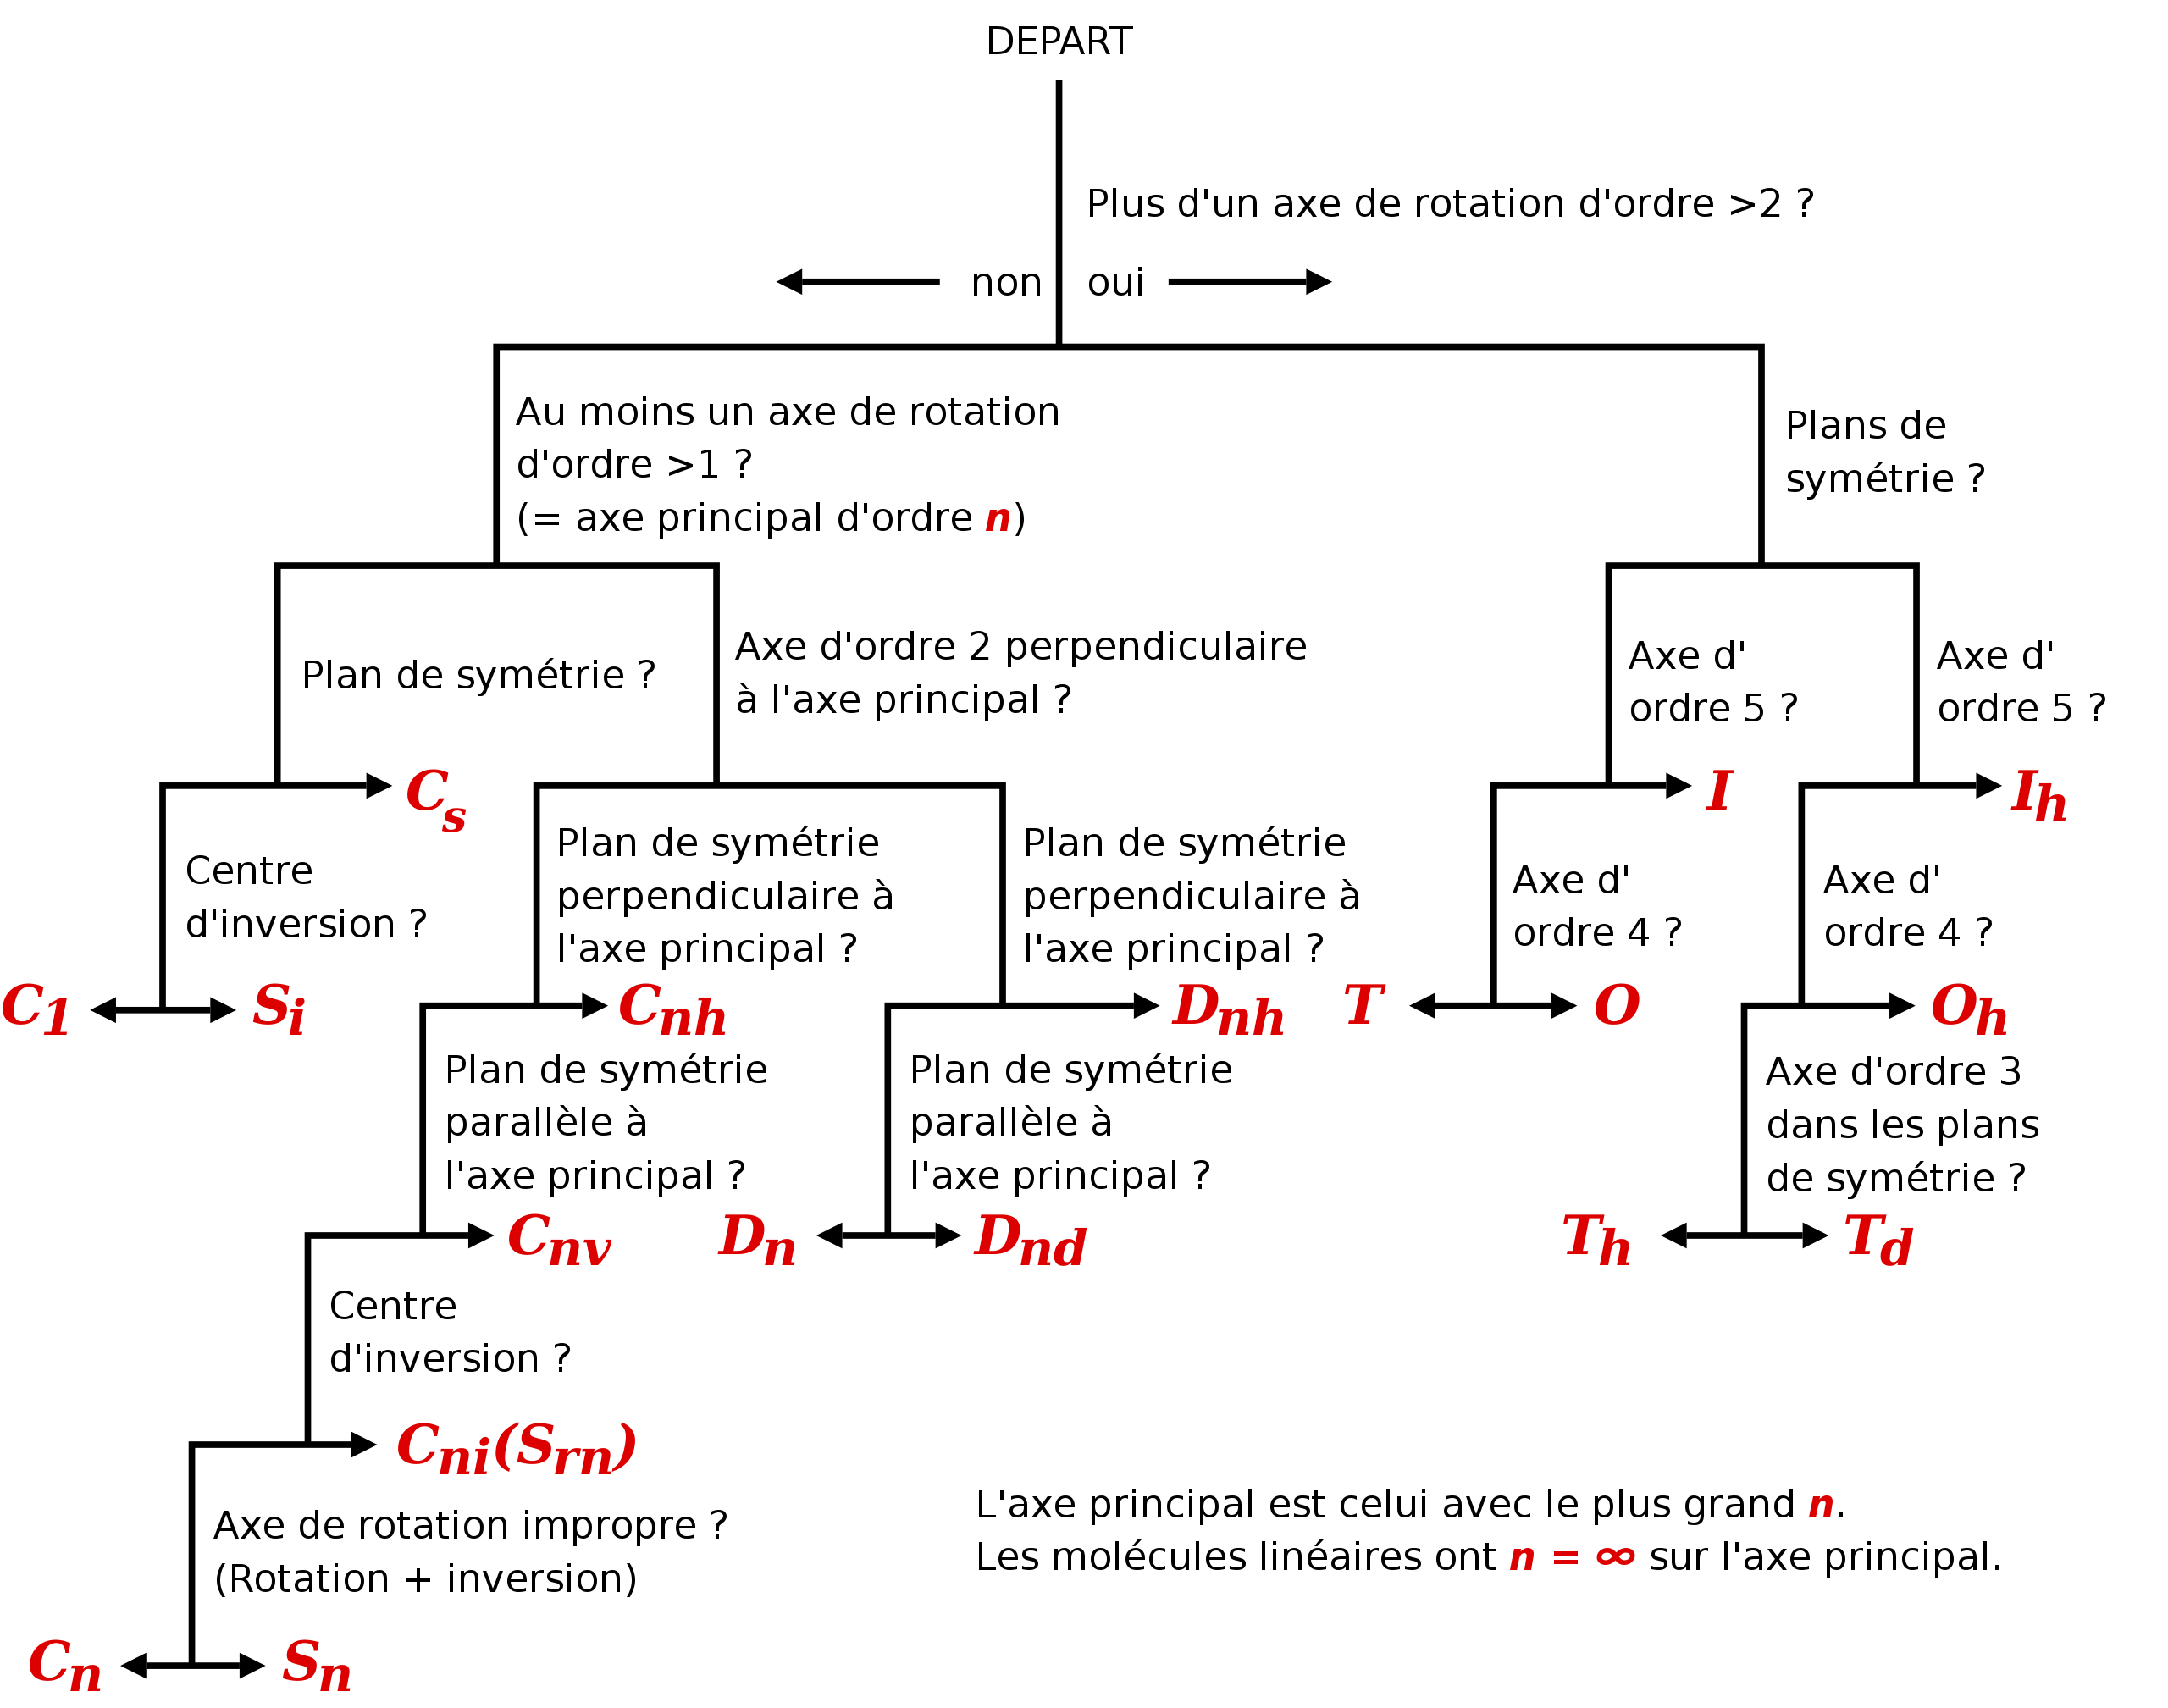
\includegraphics[scale=0.15]{groupe_chimie.png}
    \caption{群论与化学(图片源自法语wiki)}
    \label{myref:groupechimie}
  \end{figure}

  \part{附录}
  \appendix
  \chapter{114}
  \chapter{附录:三段论}
  \chapter{附录:证明方法}
  \chapter{代码}

  \printindex
\end{document}

